\documentclass[twoside]{book}

% Packages required by doxygen
\usepackage{fixltx2e}
\usepackage{calc}
\usepackage{doxygen}
\usepackage[export]{adjustbox} % also loads graphicx
\usepackage{graphicx}
\usepackage[utf8]{inputenc}
\usepackage{makeidx}
\usepackage{multicol}
\usepackage{multirow}
\PassOptionsToPackage{warn}{textcomp}
\usepackage{textcomp}
\usepackage[nointegrals]{wasysym}
\usepackage[table]{xcolor}

% Font selection
\usepackage[T1]{fontenc}
\usepackage[scaled=.90]{helvet}
\usepackage{courier}
\usepackage{amssymb}
\usepackage{sectsty}
\renewcommand{\familydefault}{\sfdefault}
\allsectionsfont{%
  \fontseries{bc}\selectfont%
  \color{darkgray}%
}
\renewcommand{\DoxyLabelFont}{%
  \fontseries{bc}\selectfont%
  \color{darkgray}%
}
\newcommand{\+}{\discretionary{\mbox{\scriptsize$\hookleftarrow$}}{}{}}

% Page & text layout
\usepackage{geometry}
\geometry{%
  a4paper,%
  top=2.5cm,%
  bottom=2.5cm,%
  left=2.5cm,%
  right=2.5cm%
}
\tolerance=750
\hfuzz=15pt
\hbadness=750
\setlength{\emergencystretch}{15pt}
\setlength{\parindent}{0cm}
\setlength{\parskip}{3ex plus 2ex minus 2ex}
\makeatletter
\renewcommand{\paragraph}{%
  \@startsection{paragraph}{4}{0ex}{-1.0ex}{1.0ex}{%
    \normalfont\normalsize\bfseries\SS@parafont%
  }%
}
\renewcommand{\subparagraph}{%
  \@startsection{subparagraph}{5}{0ex}{-1.0ex}{1.0ex}{%
    \normalfont\normalsize\bfseries\SS@subparafont%
  }%
}
\makeatother

% Headers & footers
\usepackage{fancyhdr}
\pagestyle{fancyplain}
\fancyhead[LE]{\fancyplain{}{\bfseries\thepage}}
\fancyhead[CE]{\fancyplain{}{}}
\fancyhead[RE]{\fancyplain{}{\bfseries\leftmark}}
\fancyhead[LO]{\fancyplain{}{\bfseries\rightmark}}
\fancyhead[CO]{\fancyplain{}{}}
\fancyhead[RO]{\fancyplain{}{\bfseries\thepage}}
\fancyfoot[LE]{\fancyplain{}{}}
\fancyfoot[CE]{\fancyplain{}{}}
\fancyfoot[RE]{\fancyplain{}{\bfseries\scriptsize Generated by Doxygen }}
\fancyfoot[LO]{\fancyplain{}{\bfseries\scriptsize Generated by Doxygen }}
\fancyfoot[CO]{\fancyplain{}{}}
\fancyfoot[RO]{\fancyplain{}{}}
\renewcommand{\footrulewidth}{0.4pt}
\renewcommand{\chaptermark}[1]{%
  \markboth{#1}{}%
}
\renewcommand{\sectionmark}[1]{%
  \markright{\thesection\ #1}%
}

% Indices & bibliography
\usepackage{natbib}
\usepackage[titles]{tocloft}
\setcounter{tocdepth}{3}
\setcounter{secnumdepth}{5}
\makeindex

% Hyperlinks (required, but should be loaded last)
\usepackage{ifpdf}
\ifpdf
  \usepackage[pdftex,pagebackref=true]{hyperref}
\else
  \usepackage[ps2pdf,pagebackref=true]{hyperref}
\fi
\hypersetup{%
  colorlinks=true,%
  linkcolor=blue,%
  citecolor=blue,%
  unicode%
}

% Custom commands
\newcommand{\clearemptydoublepage}{%
  \newpage{\pagestyle{empty}\cleardoublepage}%
}

\usepackage{caption}
\captionsetup{labelsep=space,justification=centering,font={bf},singlelinecheck=off,skip=4pt,position=top}

%===== C O N T E N T S =====

\begin{document}

% Titlepage & ToC
\hypersetup{pageanchor=false,
             bookmarksnumbered=true,
             pdfencoding=unicode
            }
\pagenumbering{roman}
\begin{titlepage}
\vspace*{7cm}
\begin{center}%
{\Large Simon\+Says }\\
\vspace*{1cm}
{\large Generated by Doxygen 1.8.11}\\
\end{center}
\end{titlepage}
\clearemptydoublepage
\tableofcontents
\clearemptydoublepage
\pagenumbering{arabic}
\hypersetup{pageanchor=true}

%--- Begin generated contents ---
\chapter{Juego Simon\+Says}
\label{index}\hypertarget{index}{}{\bfseries Introduction}

This user manual describes the C\+M\+S\+IS D\+SP software library, a suite of common signal processing functions for use on Cortex-\/M processor based devices.

The library is divided into a number of functions each covering a specific category\+:
\begin{DoxyItemize}
\item Basic math functions
\item Fast math functions
\item Complex math functions
\item Filters
\item Matrix functions
\item Transforms
\item Motor control functions
\item Statistical functions
\item Support functions
\item Interpolation functions
\end{DoxyItemize}

The library has separate functions for operating on 8-\/bit integers, 16-\/bit integers, 32-\/bit integer and 32-\/bit floating-\/point values.

{\bfseries Using the Library}

The library installer contains prebuilt versions of the libraries in the {\ttfamily Lib} folder.
\begin{DoxyItemize}
\item arm\+\_\+cortex\+M4lf\+\_\+math.\+lib (Little endian and Floating Point Unit on Cortex-\/\+M4)
\item arm\+\_\+cortex\+M4bf\+\_\+math.\+lib (Big endian and Floating Point Unit on Cortex-\/\+M4)
\item arm\+\_\+cortex\+M4l\+\_\+math.\+lib (Little endian on Cortex-\/\+M4)
\item arm\+\_\+cortex\+M4b\+\_\+math.\+lib (Big endian on Cortex-\/\+M4)
\item arm\+\_\+cortex\+M3l\+\_\+math.\+lib (Little endian on Cortex-\/\+M3)
\item arm\+\_\+cortex\+M3b\+\_\+math.\+lib (Big endian on Cortex-\/\+M3)
\item arm\+\_\+cortex\+M0l\+\_\+math.\+lib (Little endian on Cortex-\/\+M0)
\item arm\+\_\+cortex\+M0b\+\_\+math.\+lib (Big endian on Cortex-\/\+M3)
\end{DoxyItemize}

The library functions are declared in the public file {\ttfamily \hyperlink{arm__math_8h}{arm\+\_\+math.\+h}} which is placed in the {\ttfamily Include} folder. Simply include this file and link the appropriate library in the application and begin calling the library functions. The Library supports single public header file {\ttfamily  \hyperlink{arm__math_8h}{arm\+\_\+math.\+h}} for Cortex-\/\+M4/\+M3/\+M0 with little endian and big endian. Same header file will be used for floating point unit(\+F\+P\+U) variants. Define the appropriate pre processor M\+A\+C\+RO A\+R\+M\+\_\+\+M\+A\+T\+H\+\_\+\+C\+M4 or A\+R\+M\+\_\+\+M\+A\+T\+H\+\_\+\+C\+M3 or A\+R\+M\+\_\+\+M\+A\+T\+H\+\_\+\+C\+M0 or A\+R\+M\+\_\+\+M\+A\+T\+H\+\_\+\+C\+M0\+P\+L\+US depending on the target processor in the application.

{\bfseries Examples}

The library ships with a number of examples which demonstrate how to use the library functions.

{\bfseries Toolchain Support}

The library has been developed and tested with M\+D\+K-\/\+A\+RM version 4.\+60. The library is being tested in G\+CC and I\+AR toolchains and updates on this activity will be made available shortly.

{\bfseries Building the Library}

The library installer contains project files to re build libraries on M\+DK Tool chain in the {\ttfamily C\+M\+S\+IS\textbackslash{}D\+S\+P\+\_\+\+Lib\textbackslash{}Source\textbackslash{}A\+RM} folder.
\begin{DoxyItemize}
\item arm\+\_\+cortex\+M0b\+\_\+math.\+uvproj
\item arm\+\_\+cortex\+M0l\+\_\+math.\+uvproj
\item arm\+\_\+cortex\+M3b\+\_\+math.\+uvproj
\item arm\+\_\+cortex\+M3l\+\_\+math.\+uvproj
\item arm\+\_\+cortex\+M4b\+\_\+math.\+uvproj
\item arm\+\_\+cortex\+M4l\+\_\+math.\+uvproj
\item arm\+\_\+cortex\+M4bf\+\_\+math.\+uvproj
\item arm\+\_\+cortex\+M4lf\+\_\+math.\+uvproj
\end{DoxyItemize}

The project can be built by opening the appropriate project in M\+D\+K-\/\+A\+RM 4.\+60 chain and defining the optional pre processor M\+A\+C\+R\+Os detailed above.

{\bfseries Pre-\/processor Macros}

Each library project have differant pre-\/processor macros.


\begin{DoxyItemize}
\item U\+N\+A\+L\+I\+G\+N\+E\+D\+\_\+\+S\+U\+P\+P\+O\+R\+T\+\_\+\+D\+I\+S\+A\+B\+LE\+:
\end{DoxyItemize}

Define macro U\+N\+A\+L\+I\+G\+N\+E\+D\+\_\+\+S\+U\+P\+P\+O\+R\+T\+\_\+\+D\+I\+S\+A\+B\+LE, If the silicon does not support unaligned memory access


\begin{DoxyItemize}
\item A\+R\+M\+\_\+\+M\+A\+T\+H\+\_\+\+B\+I\+G\+\_\+\+E\+N\+D\+I\+AN\+:
\end{DoxyItemize}

Define macro A\+R\+M\+\_\+\+M\+A\+T\+H\+\_\+\+B\+I\+G\+\_\+\+E\+N\+D\+I\+AN to build the library for big endian targets. By default library builds for little endian targets.


\begin{DoxyItemize}
\item A\+R\+M\+\_\+\+M\+A\+T\+H\+\_\+\+M\+A\+T\+R\+I\+X\+\_\+\+C\+H\+E\+CK\+:
\end{DoxyItemize}

Define macro A\+R\+M\+\_\+\+M\+A\+T\+H\+\_\+\+M\+A\+T\+R\+I\+X\+\_\+\+C\+H\+E\+CK for checking on the input and output sizes of matrices


\begin{DoxyItemize}
\item A\+R\+M\+\_\+\+M\+A\+T\+H\+\_\+\+R\+O\+U\+N\+D\+I\+NG\+:
\end{DoxyItemize}

Define macro A\+R\+M\+\_\+\+M\+A\+T\+H\+\_\+\+R\+O\+U\+N\+D\+I\+NG for rounding on support functions


\begin{DoxyItemize}
\item A\+R\+M\+\_\+\+M\+A\+T\+H\+\_\+\+C\+Mx\+:
\end{DoxyItemize}

Define macro A\+R\+M\+\_\+\+M\+A\+T\+H\+\_\+\+C\+M4 for building the library on Cortex-\/\+M4 target, A\+R\+M\+\_\+\+M\+A\+T\+H\+\_\+\+C\+M3 for building library on Cortex-\/\+M3 target and A\+R\+M\+\_\+\+M\+A\+T\+H\+\_\+\+C\+M0 for building library on cortex-\/\+M0 target, A\+R\+M\+\_\+\+M\+A\+T\+H\+\_\+\+C\+M0\+P\+L\+US for building library on cortex-\/\+M0+ target.


\begin{DoxyItemize}
\item \+\_\+\+\_\+\+F\+P\+U\+\_\+\+P\+R\+E\+S\+E\+NT\+:
\end{DoxyItemize}

Initialize macro \+\_\+\+\_\+\+F\+P\+U\+\_\+\+P\+R\+E\+S\+E\+NT = 1 when building on F\+PU supported Targets. Enable this macro for M4bf and M4lf libraries

{\bfseries Copyright Notice}

Copyright (C) 2010-\/2013 A\+RM Limited. All rights reserved. 
\chapter{Module Index}
\section{Modules}
Here is a list of all modules\+:\begin{DoxyCompactList}
\item \contentsline{section}{Hardware}{\pageref{group__hardware}}{}
\item \contentsline{section}{Operaciones}{\pageref{group__operaciones}}{}
\end{DoxyCompactList}

\chapter{Class Index}
\section{Estructura de datos}
Lista de estructuras con una breve descripción\+:\begin{DoxyCompactList}
\item\contentsline{section}{\hyperlink{struct__mci__card__struct}{\+\_\+mci\+\_\+card\+\_\+struct} }{\pageref{struct__mci__card__struct}}{}
\item\contentsline{section}{\hyperlink{struct__sdif__device}{\+\_\+sdif\+\_\+device} \\*S\+D\+IO device type }{\pageref{struct__sdif__device}}{}
\item\contentsline{section}{\hyperlink{struct_a_d_c___c_l_o_c_k___s_e_t_u_p___t}{A\+D\+C\+\_\+\+C\+L\+O\+C\+K\+\_\+\+S\+E\+T\+U\+P\+\_\+T} }{\pageref{struct_a_d_c___c_l_o_c_k___s_e_t_u_p___t}}{}
\item\contentsline{section}{\hyperlink{struct_a_e_s___a_p_i___t}{A\+E\+S\+\_\+\+A\+P\+I\+\_\+T} \\*L\+P\+C18\+X\+X\+\_\+43\+XX A\+ES A\+PI structure }{\pageref{struct_a_e_s___a_p_i___t}}{}
\item\contentsline{section}{\hyperlink{union_a_p_s_r___type}{A\+P\+S\+R\+\_\+\+Type} \\*Union type to access the Application Program Status Register (A\+P\+SR) }{\pageref{union_a_p_s_r___type}}{}
\item\contentsline{section}{\hyperlink{structarm__bilinear__interp__instance__f32}{arm\+\_\+bilinear\+\_\+interp\+\_\+instance\+\_\+f32} \\*Instance structure for the floating-\/point bilinear interpolation function }{\pageref{structarm__bilinear__interp__instance__f32}}{}
\item\contentsline{section}{\hyperlink{structarm__bilinear__interp__instance__q15}{arm\+\_\+bilinear\+\_\+interp\+\_\+instance\+\_\+q15} \\*Instance structure for the Q15 bilinear interpolation function }{\pageref{structarm__bilinear__interp__instance__q15}}{}
\item\contentsline{section}{\hyperlink{structarm__bilinear__interp__instance__q31}{arm\+\_\+bilinear\+\_\+interp\+\_\+instance\+\_\+q31} \\*Instance structure for the Q31 bilinear interpolation function }{\pageref{structarm__bilinear__interp__instance__q31}}{}
\item\contentsline{section}{\hyperlink{structarm__bilinear__interp__instance__q7}{arm\+\_\+bilinear\+\_\+interp\+\_\+instance\+\_\+q7} \\*Instance structure for the Q15 bilinear interpolation function }{\pageref{structarm__bilinear__interp__instance__q7}}{}
\item\contentsline{section}{\hyperlink{structarm__biquad__cas__df1__32x64__ins__q31}{arm\+\_\+biquad\+\_\+cas\+\_\+df1\+\_\+32x64\+\_\+ins\+\_\+q31} \\*Instance structure for the high precision Q31 Biquad cascade filter }{\pageref{structarm__biquad__cas__df1__32x64__ins__q31}}{}
\item\contentsline{section}{\hyperlink{structarm__biquad__cascade__df2_t__instance__f32}{arm\+\_\+biquad\+\_\+cascade\+\_\+df2\+T\+\_\+instance\+\_\+f32} \\*Instance structure for the floating-\/point transposed direct form II Biquad cascade filter }{\pageref{structarm__biquad__cascade__df2_t__instance__f32}}{}
\item\contentsline{section}{\hyperlink{structarm__biquad__casd__df1__inst__f32}{arm\+\_\+biquad\+\_\+casd\+\_\+df1\+\_\+inst\+\_\+f32} \\*Instance structure for the floating-\/point Biquad cascade filter }{\pageref{structarm__biquad__casd__df1__inst__f32}}{}
\item\contentsline{section}{\hyperlink{structarm__biquad__casd__df1__inst__q15}{arm\+\_\+biquad\+\_\+casd\+\_\+df1\+\_\+inst\+\_\+q15} \\*Instance structure for the Q15 Biquad cascade filter }{\pageref{structarm__biquad__casd__df1__inst__q15}}{}
\item\contentsline{section}{\hyperlink{structarm__biquad__casd__df1__inst__q31}{arm\+\_\+biquad\+\_\+casd\+\_\+df1\+\_\+inst\+\_\+q31} \\*Instance structure for the Q31 Biquad cascade filter }{\pageref{structarm__biquad__casd__df1__inst__q31}}{}
\item\contentsline{section}{\hyperlink{structarm__cfft__instance__f32}{arm\+\_\+cfft\+\_\+instance\+\_\+f32} \\*Instance structure for the floating-\/point C\+F\+F\+T/\+C\+I\+F\+FT function }{\pageref{structarm__cfft__instance__f32}}{}
\item\contentsline{section}{\hyperlink{structarm__cfft__radix2__instance__f32}{arm\+\_\+cfft\+\_\+radix2\+\_\+instance\+\_\+f32} \\*Instance structure for the floating-\/point C\+F\+F\+T/\+C\+I\+F\+FT function }{\pageref{structarm__cfft__radix2__instance__f32}}{}
\item\contentsline{section}{\hyperlink{structarm__cfft__radix2__instance__q15}{arm\+\_\+cfft\+\_\+radix2\+\_\+instance\+\_\+q15} \\*Instance structure for the Q15 C\+F\+F\+T/\+C\+I\+F\+FT function }{\pageref{structarm__cfft__radix2__instance__q15}}{}
\item\contentsline{section}{\hyperlink{structarm__cfft__radix2__instance__q31}{arm\+\_\+cfft\+\_\+radix2\+\_\+instance\+\_\+q31} \\*Instance structure for the Radix-\/2 Q31 C\+F\+F\+T/\+C\+I\+F\+FT function }{\pageref{structarm__cfft__radix2__instance__q31}}{}
\item\contentsline{section}{\hyperlink{structarm__cfft__radix4__instance__f32}{arm\+\_\+cfft\+\_\+radix4\+\_\+instance\+\_\+f32} \\*Instance structure for the floating-\/point C\+F\+F\+T/\+C\+I\+F\+FT function }{\pageref{structarm__cfft__radix4__instance__f32}}{}
\item\contentsline{section}{\hyperlink{structarm__cfft__radix4__instance__q15}{arm\+\_\+cfft\+\_\+radix4\+\_\+instance\+\_\+q15} \\*Instance structure for the Q15 C\+F\+F\+T/\+C\+I\+F\+FT function }{\pageref{structarm__cfft__radix4__instance__q15}}{}
\item\contentsline{section}{\hyperlink{structarm__cfft__radix4__instance__q31}{arm\+\_\+cfft\+\_\+radix4\+\_\+instance\+\_\+q31} \\*Instance structure for the Q31 C\+F\+F\+T/\+C\+I\+F\+FT function }{\pageref{structarm__cfft__radix4__instance__q31}}{}
\item\contentsline{section}{\hyperlink{structarm__dct4__instance__f32}{arm\+\_\+dct4\+\_\+instance\+\_\+f32} \\*Instance structure for the floating-\/point D\+C\+T4/\+I\+D\+C\+T4 function }{\pageref{structarm__dct4__instance__f32}}{}
\item\contentsline{section}{\hyperlink{structarm__dct4__instance__q15}{arm\+\_\+dct4\+\_\+instance\+\_\+q15} \\*Instance structure for the Q15 D\+C\+T4/\+I\+D\+C\+T4 function }{\pageref{structarm__dct4__instance__q15}}{}
\item\contentsline{section}{\hyperlink{structarm__dct4__instance__q31}{arm\+\_\+dct4\+\_\+instance\+\_\+q31} \\*Instance structure for the Q31 D\+C\+T4/\+I\+D\+C\+T4 function }{\pageref{structarm__dct4__instance__q31}}{}
\item\contentsline{section}{\hyperlink{structarm__fir__decimate__instance__f32}{arm\+\_\+fir\+\_\+decimate\+\_\+instance\+\_\+f32} \\*Instance structure for the floating-\/point F\+IR decimator }{\pageref{structarm__fir__decimate__instance__f32}}{}
\item\contentsline{section}{\hyperlink{structarm__fir__decimate__instance__q15}{arm\+\_\+fir\+\_\+decimate\+\_\+instance\+\_\+q15} \\*Instance structure for the Q15 F\+IR decimator }{\pageref{structarm__fir__decimate__instance__q15}}{}
\item\contentsline{section}{\hyperlink{structarm__fir__decimate__instance__q31}{arm\+\_\+fir\+\_\+decimate\+\_\+instance\+\_\+q31} \\*Instance structure for the Q31 F\+IR decimator }{\pageref{structarm__fir__decimate__instance__q31}}{}
\item\contentsline{section}{\hyperlink{structarm__fir__instance__f32}{arm\+\_\+fir\+\_\+instance\+\_\+f32} \\*Instance structure for the floating-\/point F\+IR filter }{\pageref{structarm__fir__instance__f32}}{}
\item\contentsline{section}{\hyperlink{structarm__fir__instance__q15}{arm\+\_\+fir\+\_\+instance\+\_\+q15} \\*Instance structure for the Q15 F\+IR filter }{\pageref{structarm__fir__instance__q15}}{}
\item\contentsline{section}{\hyperlink{structarm__fir__instance__q31}{arm\+\_\+fir\+\_\+instance\+\_\+q31} \\*Instance structure for the Q31 F\+IR filter }{\pageref{structarm__fir__instance__q31}}{}
\item\contentsline{section}{\hyperlink{structarm__fir__instance__q7}{arm\+\_\+fir\+\_\+instance\+\_\+q7} \\*Instance structure for the Q7 F\+IR filter }{\pageref{structarm__fir__instance__q7}}{}
\item\contentsline{section}{\hyperlink{structarm__fir__interpolate__instance__f32}{arm\+\_\+fir\+\_\+interpolate\+\_\+instance\+\_\+f32} \\*Instance structure for the floating-\/point F\+IR interpolator }{\pageref{structarm__fir__interpolate__instance__f32}}{}
\item\contentsline{section}{\hyperlink{structarm__fir__interpolate__instance__q15}{arm\+\_\+fir\+\_\+interpolate\+\_\+instance\+\_\+q15} \\*Instance structure for the Q15 F\+IR interpolator }{\pageref{structarm__fir__interpolate__instance__q15}}{}
\item\contentsline{section}{\hyperlink{structarm__fir__interpolate__instance__q31}{arm\+\_\+fir\+\_\+interpolate\+\_\+instance\+\_\+q31} \\*Instance structure for the Q31 F\+IR interpolator }{\pageref{structarm__fir__interpolate__instance__q31}}{}
\item\contentsline{section}{\hyperlink{structarm__fir__lattice__instance__f32}{arm\+\_\+fir\+\_\+lattice\+\_\+instance\+\_\+f32} \\*Instance structure for the floating-\/point F\+IR lattice filter }{\pageref{structarm__fir__lattice__instance__f32}}{}
\item\contentsline{section}{\hyperlink{structarm__fir__lattice__instance__q15}{arm\+\_\+fir\+\_\+lattice\+\_\+instance\+\_\+q15} \\*Instance structure for the Q15 F\+IR lattice filter }{\pageref{structarm__fir__lattice__instance__q15}}{}
\item\contentsline{section}{\hyperlink{structarm__fir__lattice__instance__q31}{arm\+\_\+fir\+\_\+lattice\+\_\+instance\+\_\+q31} \\*Instance structure for the Q31 F\+IR lattice filter }{\pageref{structarm__fir__lattice__instance__q31}}{}
\item\contentsline{section}{\hyperlink{structarm__fir__sparse__instance__f32}{arm\+\_\+fir\+\_\+sparse\+\_\+instance\+\_\+f32} \\*Instance structure for the floating-\/point sparse F\+IR filter }{\pageref{structarm__fir__sparse__instance__f32}}{}
\item\contentsline{section}{\hyperlink{structarm__fir__sparse__instance__q15}{arm\+\_\+fir\+\_\+sparse\+\_\+instance\+\_\+q15} \\*Instance structure for the Q15 sparse F\+IR filter }{\pageref{structarm__fir__sparse__instance__q15}}{}
\item\contentsline{section}{\hyperlink{structarm__fir__sparse__instance__q31}{arm\+\_\+fir\+\_\+sparse\+\_\+instance\+\_\+q31} \\*Instance structure for the Q31 sparse F\+IR filter }{\pageref{structarm__fir__sparse__instance__q31}}{}
\item\contentsline{section}{\hyperlink{structarm__fir__sparse__instance__q7}{arm\+\_\+fir\+\_\+sparse\+\_\+instance\+\_\+q7} \\*Instance structure for the Q7 sparse F\+IR filter }{\pageref{structarm__fir__sparse__instance__q7}}{}
\item\contentsline{section}{\hyperlink{structarm__iir__lattice__instance__f32}{arm\+\_\+iir\+\_\+lattice\+\_\+instance\+\_\+f32} \\*Instance structure for the floating-\/point I\+IR lattice filter }{\pageref{structarm__iir__lattice__instance__f32}}{}
\item\contentsline{section}{\hyperlink{structarm__iir__lattice__instance__q15}{arm\+\_\+iir\+\_\+lattice\+\_\+instance\+\_\+q15} \\*Instance structure for the Q15 I\+IR lattice filter }{\pageref{structarm__iir__lattice__instance__q15}}{}
\item\contentsline{section}{\hyperlink{structarm__iir__lattice__instance__q31}{arm\+\_\+iir\+\_\+lattice\+\_\+instance\+\_\+q31} \\*Instance structure for the Q31 I\+IR lattice filter }{\pageref{structarm__iir__lattice__instance__q31}}{}
\item\contentsline{section}{\hyperlink{structarm__linear__interp__instance__f32}{arm\+\_\+linear\+\_\+interp\+\_\+instance\+\_\+f32} \\*Instance structure for the floating-\/point Linear Interpolate function }{\pageref{structarm__linear__interp__instance__f32}}{}
\item\contentsline{section}{\hyperlink{structarm__lms__instance__f32}{arm\+\_\+lms\+\_\+instance\+\_\+f32} \\*Instance structure for the floating-\/point L\+MS filter }{\pageref{structarm__lms__instance__f32}}{}
\item\contentsline{section}{\hyperlink{structarm__lms__instance__q15}{arm\+\_\+lms\+\_\+instance\+\_\+q15} \\*Instance structure for the Q15 L\+MS filter }{\pageref{structarm__lms__instance__q15}}{}
\item\contentsline{section}{\hyperlink{structarm__lms__instance__q31}{arm\+\_\+lms\+\_\+instance\+\_\+q31} \\*Instance structure for the Q31 L\+MS filter }{\pageref{structarm__lms__instance__q31}}{}
\item\contentsline{section}{\hyperlink{structarm__lms__norm__instance__f32}{arm\+\_\+lms\+\_\+norm\+\_\+instance\+\_\+f32} \\*Instance structure for the floating-\/point normalized L\+MS filter }{\pageref{structarm__lms__norm__instance__f32}}{}
\item\contentsline{section}{\hyperlink{structarm__lms__norm__instance__q15}{arm\+\_\+lms\+\_\+norm\+\_\+instance\+\_\+q15} \\*Instance structure for the Q15 normalized L\+MS filter }{\pageref{structarm__lms__norm__instance__q15}}{}
\item\contentsline{section}{\hyperlink{structarm__lms__norm__instance__q31}{arm\+\_\+lms\+\_\+norm\+\_\+instance\+\_\+q31} \\*Instance structure for the Q31 normalized L\+MS filter }{\pageref{structarm__lms__norm__instance__q31}}{}
\item\contentsline{section}{\hyperlink{structarm__matrix__instance__f32}{arm\+\_\+matrix\+\_\+instance\+\_\+f32} \\*Instance structure for the floating-\/point matrix structure }{\pageref{structarm__matrix__instance__f32}}{}
\item\contentsline{section}{\hyperlink{structarm__matrix__instance__q15}{arm\+\_\+matrix\+\_\+instance\+\_\+q15} \\*Instance structure for the Q15 matrix structure }{\pageref{structarm__matrix__instance__q15}}{}
\item\contentsline{section}{\hyperlink{structarm__matrix__instance__q31}{arm\+\_\+matrix\+\_\+instance\+\_\+q31} \\*Instance structure for the Q31 matrix structure }{\pageref{structarm__matrix__instance__q31}}{}
\item\contentsline{section}{\hyperlink{structarm__pid__instance__f32}{arm\+\_\+pid\+\_\+instance\+\_\+f32} \\*Instance structure for the floating-\/point P\+ID Control }{\pageref{structarm__pid__instance__f32}}{}
\item\contentsline{section}{\hyperlink{structarm__pid__instance__q15}{arm\+\_\+pid\+\_\+instance\+\_\+q15} \\*Instance structure for the Q15 P\+ID Control }{\pageref{structarm__pid__instance__q15}}{}
\item\contentsline{section}{\hyperlink{structarm__pid__instance__q31}{arm\+\_\+pid\+\_\+instance\+\_\+q31} \\*Instance structure for the Q31 P\+ID Control }{\pageref{structarm__pid__instance__q31}}{}
\item\contentsline{section}{\hyperlink{structarm__rfft__fast__instance__f32}{arm\+\_\+rfft\+\_\+fast\+\_\+instance\+\_\+f32} \\*Instance structure for the floating-\/point R\+F\+F\+T/\+R\+I\+F\+FT function }{\pageref{structarm__rfft__fast__instance__f32}}{}
\item\contentsline{section}{\hyperlink{structarm__rfft__instance__f32}{arm\+\_\+rfft\+\_\+instance\+\_\+f32} \\*Instance structure for the floating-\/point R\+F\+F\+T/\+R\+I\+F\+FT function }{\pageref{structarm__rfft__instance__f32}}{}
\item\contentsline{section}{\hyperlink{structarm__rfft__instance__q15}{arm\+\_\+rfft\+\_\+instance\+\_\+q15} \\*Instance structure for the Q15 R\+F\+F\+T/\+R\+I\+F\+FT function }{\pageref{structarm__rfft__instance__q15}}{}
\item\contentsline{section}{\hyperlink{structarm__rfft__instance__q31}{arm\+\_\+rfft\+\_\+instance\+\_\+q31} \\*Instance structure for the Q31 R\+F\+F\+T/\+R\+I\+F\+FT function }{\pageref{structarm__rfft__instance__q31}}{}
\item\contentsline{section}{\hyperlink{struct_c_c_a_n___i_f___t}{C\+C\+A\+N\+\_\+\+I\+F\+\_\+T} \\*C\+C\+AN message interface register block structure }{\pageref{struct_c_c_a_n___i_f___t}}{}
\item\contentsline{section}{\hyperlink{struct_c_c_a_n___m_s_g___o_b_j___t}{C\+C\+A\+N\+\_\+\+M\+S\+G\+\_\+\+O\+B\+J\+\_\+T} \\*C\+AN message object structure }{\pageref{struct_c_c_a_n___m_s_g___o_b_j___t}}{}
\item\contentsline{section}{\hyperlink{struct_c_c_u___c_f_g_s_t_a_t___t}{C\+C\+U\+\_\+\+C\+F\+G\+S\+T\+A\+T\+\_\+T} \\*C\+CU clock config/status register pair }{\pageref{struct_c_c_u___c_f_g_s_t_a_t___t}}{}
\item\contentsline{section}{\hyperlink{struct_c_g_u___p_l_l___r_e_g___t}{C\+G\+U\+\_\+\+P\+L\+L\+\_\+\+R\+E\+G\+\_\+T} }{\pageref{struct_c_g_u___p_l_l___r_e_g___t}}{}
\item\contentsline{section}{\hyperlink{struct_c_g_u___u_s_b_a_u_d_i_o___p_l_l___s_e_t_u_p___t}{C\+G\+U\+\_\+\+U\+S\+B\+A\+U\+D\+I\+O\+\_\+\+P\+L\+L\+\_\+\+S\+E\+T\+U\+P\+\_\+T} }{\pageref{struct_c_g_u___u_s_b_a_u_d_i_o___p_l_l___s_e_t_u_p___t}}{}
\item\contentsline{section}{\hyperlink{struct_chip___s_s_p___d_a_t_a___s_e_t_u_p___t}{Chip\+\_\+\+S\+S\+P\+\_\+\+D\+A\+T\+A\+\_\+\+S\+E\+T\+U\+P\+\_\+T} }{\pageref{struct_chip___s_s_p___d_a_t_a___s_e_t_u_p___t}}{}
\item\contentsline{section}{\hyperlink{struct_c_l_k___b_a_s_e___s_t_a_t_e_s}{C\+L\+K\+\_\+\+B\+A\+S\+E\+\_\+\+S\+T\+A\+T\+ES} }{\pageref{struct_c_l_k___b_a_s_e___s_t_a_t_e_s}}{}
\item\contentsline{section}{\hyperlink{struct_c_l_k___p_e_r_i_p_h___t_o___b_a_s_e___t}{C\+L\+K\+\_\+\+P\+E\+R\+I\+P\+H\+\_\+\+T\+O\+\_\+\+B\+A\+S\+E\+\_\+T} }{\pageref{struct_c_l_k___p_e_r_i_p_h___t_o___b_a_s_e___t}}{}
\item\contentsline{section}{\hyperlink{union_c_o_n_t_r_o_l___type}{C\+O\+N\+T\+R\+O\+L\+\_\+\+Type} \\*Union type to access the Control Registers (C\+O\+N\+T\+R\+OL) }{\pageref{union_c_o_n_t_r_o_l___type}}{}
\item\contentsline{section}{\hyperlink{struct_core_debug___type}{Core\+Debug\+\_\+\+Type} \\*Structure type to access the Core Debug Register (Core\+Debug) }{\pageref{struct_core_debug___type}}{}
\item\contentsline{section}{\hyperlink{struct_c_r_s_d_c_e_g___t}{C\+R\+S\+D\+C\+E\+G\+\_\+T} }{\pageref{struct_c_r_s_d_c_e_g___t}}{}
\item\contentsline{section}{\hyperlink{struct_d_m_a___channel_handle__t}{D\+M\+A\+\_\+\+Channel\+Handle\+\_\+t} \\*D\+MA channel handle structure }{\pageref{struct_d_m_a___channel_handle__t}}{}
\item\contentsline{section}{\hyperlink{struct_d_m_a___transfer_descriptor}{D\+M\+A\+\_\+\+Transfer\+Descriptor} \\*Transfer Descriptor structure typedef }{\pageref{struct_d_m_a___transfer_descriptor}}{}
\item\contentsline{section}{\hyperlink{struct_d_w_t___type}{D\+W\+T\+\_\+\+Type} \\*Structure type to access the Data Watchpoint and Trace Register (D\+WT) }{\pageref{struct_d_w_t___type}}{}
\item\contentsline{section}{\hyperlink{struct_e_n_e_t___e_n_h_r_x_d_e_s_c___t}{E\+N\+E\+T\+\_\+\+E\+N\+H\+R\+X\+D\+E\+S\+C\+\_\+T} \\*Structure of a enhanced receive descriptor (with timestamp) }{\pageref{struct_e_n_e_t___e_n_h_r_x_d_e_s_c___t}}{}
\item\contentsline{section}{\hyperlink{struct_e_n_e_t___e_n_h_t_x_d_e_s_c___t}{E\+N\+E\+T\+\_\+\+E\+N\+H\+T\+X\+D\+E\+S\+C\+\_\+T} \\*Structure of a enhanced transmit descriptor (with timestamp) }{\pageref{struct_e_n_e_t___e_n_h_t_x_d_e_s_c___t}}{}
\item\contentsline{section}{\hyperlink{struct_e_n_e_t___r_x_d_e_s_c___t}{E\+N\+E\+T\+\_\+\+R\+X\+D\+E\+S\+C\+\_\+T} \\*Structure of a receive descriptor (without timestamp) }{\pageref{struct_e_n_e_t___r_x_d_e_s_c___t}}{}
\item\contentsline{section}{\hyperlink{struct_e_n_e_t___t_x_d_e_s_c___t}{E\+N\+E\+T\+\_\+\+T\+X\+D\+E\+S\+C\+\_\+T} \\*Structure of a transmit descriptor (without timestamp) }{\pageref{struct_e_n_e_t___t_x_d_e_s_c___t}}{}
\item\contentsline{section}{\hyperlink{struct_g_p_d_m_a___c_h___c_f_g___t}{G\+P\+D\+M\+A\+\_\+\+C\+H\+\_\+\+C\+F\+G\+\_\+T} \\*G\+P\+D\+MA structure using for D\+MA configuration }{\pageref{struct_g_p_d_m_a___c_h___c_f_g___t}}{}
\item\contentsline{section}{\hyperlink{struct_g_p_d_m_a___c_h___t}{G\+P\+D\+M\+A\+\_\+\+C\+H\+\_\+T} \\*G\+P\+D\+MA Channel register block structure }{\pageref{struct_g_p_d_m_a___c_h___t}}{}
\item\contentsline{section}{\hyperlink{struct_h_s_a_d_c_i_n_t_c_t_r_l___t}{H\+S\+A\+D\+C\+I\+N\+T\+C\+T\+R\+L\+\_\+T} \\*High speed A\+DC interrupt control structure }{\pageref{struct_h_s_a_d_c_i_n_t_c_t_r_l___t}}{}
\item\contentsline{section}{\hyperlink{structi2c__interface}{i2c\+\_\+interface} }{\pageref{structi2c__interface}}{}
\item\contentsline{section}{\hyperlink{structi2c__slave__interface}{i2c\+\_\+slave\+\_\+interface} }{\pageref{structi2c__slave__interface}}{}
\item\contentsline{section}{\hyperlink{struct_i2_c___x_f_e_r___t}{I2\+C\+\_\+\+X\+F\+E\+R\+\_\+T} \\*Master transfer data structure definitions }{\pageref{struct_i2_c___x_f_e_r___t}}{}
\item\contentsline{section}{\hyperlink{struct_i2_c_m___x_f_e_r___t}{I2\+C\+M\+\_\+\+X\+F\+E\+R\+\_\+T} \\*Master transfer data structure definitions }{\pageref{struct_i2_c_m___x_f_e_r___t}}{}
\item\contentsline{section}{\hyperlink{struct_i2_s___a_u_d_i_o___f_o_r_m_a_t___t}{I2\+S\+\_\+\+A\+U\+D\+I\+O\+\_\+\+F\+O\+R\+M\+A\+T\+\_\+T} \\*I2S Audio Format Structure }{\pageref{struct_i2_s___a_u_d_i_o___f_o_r_m_a_t___t}}{}
\item\contentsline{section}{\hyperlink{struct_i_p___e_m_c___d_y_n___c_o_n_f_i_g___t}{I\+P\+\_\+\+E\+M\+C\+\_\+\+D\+Y\+N\+\_\+\+C\+O\+N\+F\+I\+G\+\_\+T} \\*E\+MC Dynamic Configure Struct }{\pageref{struct_i_p___e_m_c___d_y_n___c_o_n_f_i_g___t}}{}
\item\contentsline{section}{\hyperlink{struct_i_p___e_m_c___d_y_n___d_e_v_i_c_e___c_o_n_f_i_g___t}{I\+P\+\_\+\+E\+M\+C\+\_\+\+D\+Y\+N\+\_\+\+D\+E\+V\+I\+C\+E\+\_\+\+C\+O\+N\+F\+I\+G\+\_\+T} \\*E\+MC Dynamic Device Configuration structure used for IP drivers }{\pageref{struct_i_p___e_m_c___d_y_n___d_e_v_i_c_e___c_o_n_f_i_g___t}}{}
\item\contentsline{section}{\hyperlink{struct_i_p___e_m_c___s_t_a_t_i_c___c_o_n_f_i_g___t}{I\+P\+\_\+\+E\+M\+C\+\_\+\+S\+T\+A\+T\+I\+C\+\_\+\+C\+O\+N\+F\+I\+G\+\_\+T} \\*E\+MC Static Configure Structure }{\pageref{struct_i_p___e_m_c___s_t_a_t_i_c___c_o_n_f_i_g___t}}{}
\item\contentsline{section}{\hyperlink{union_i_p_s_r___type}{I\+P\+S\+R\+\_\+\+Type} \\*Union type to access the Interrupt Program Status Register (I\+P\+SR) }{\pageref{union_i_p_s_r___type}}{}
\item\contentsline{section}{\hyperlink{struct_i_t_m___type}{I\+T\+M\+\_\+\+Type} \\*Structure type to access the Instrumentation Trace Macrocell Register (I\+TM) }{\pageref{struct_i_t_m___type}}{}
\item\contentsline{section}{\hyperlink{struct_l_c_d___c_o_n_f_i_g___t}{L\+C\+D\+\_\+\+C\+O\+N\+F\+I\+G\+\_\+T} \\*A structure for L\+CD Configuration }{\pageref{struct_l_c_d___c_o_n_f_i_g___t}}{}
\item\contentsline{section}{\hyperlink{struct_l_c_d___p_a_l_e_t_t_e___e_n_t_r_y___t}{L\+C\+D\+\_\+\+P\+A\+L\+E\+T\+T\+E\+\_\+\+E\+N\+T\+R\+Y\+\_\+T} \\*L\+CD Palette entry format }{\pageref{struct_l_c_d___p_a_l_e_t_t_e___e_n_t_r_y___t}}{}
\item\contentsline{section}{\hyperlink{struct_l_p_c___a_d_c___t}{L\+P\+C\+\_\+\+A\+D\+C\+\_\+T} \\*10 or 12-\/bit A\+DC register block structure }{\pageref{struct_l_p_c___a_d_c___t}}{}
\item\contentsline{section}{\hyperlink{struct_l_p_c___a_t_i_m_e_r___t}{L\+P\+C\+\_\+\+A\+T\+I\+M\+E\+R\+\_\+T} \\*Alarm Timer register block structure }{\pageref{struct_l_p_c___a_t_i_m_e_r___t}}{}
\item\contentsline{section}{\hyperlink{struct_l_p_c___c_c_a_n___t}{L\+P\+C\+\_\+\+C\+C\+A\+N\+\_\+T} \\*C\+C\+AN Controller Area Network register block structure }{\pageref{struct_l_p_c___c_c_a_n___t}}{}
\item\contentsline{section}{\hyperlink{struct_l_p_c___c_c_u1___t}{L\+P\+C\+\_\+\+C\+C\+U1\+\_\+T} \\*C\+C\+U1 register block structure }{\pageref{struct_l_p_c___c_c_u1___t}}{}
\item\contentsline{section}{\hyperlink{struct_l_p_c___c_c_u2___t}{L\+P\+C\+\_\+\+C\+C\+U2\+\_\+T} \\*C\+C\+U2 register block structure }{\pageref{struct_l_p_c___c_c_u2___t}}{}
\item\contentsline{section}{\hyperlink{struct_l_p_c___c_g_u___t}{L\+P\+C\+\_\+\+C\+G\+U\+\_\+T} \\*L\+P\+C18\+X\+X/43\+XX C\+GU register block structure }{\pageref{struct_l_p_c___c_g_u___t}}{}
\item\contentsline{section}{\hyperlink{struct_l_p_c___c_r_e_g___t}{L\+P\+C\+\_\+\+C\+R\+E\+G\+\_\+T} \\*C\+R\+EG Register Block }{\pageref{struct_l_p_c___c_r_e_g___t}}{}
\item\contentsline{section}{\hyperlink{struct_l_p_c___d_a_c___t}{L\+P\+C\+\_\+\+D\+A\+C\+\_\+T} \\*D\+AC register block structure }{\pageref{struct_l_p_c___d_a_c___t}}{}
\item\contentsline{section}{\hyperlink{struct_l_p_c___e_e_p_r_o_m___t}{L\+P\+C\+\_\+\+E\+E\+P\+R\+O\+M\+\_\+T} \\*E\+E\+P\+R\+OM register block structure }{\pageref{struct_l_p_c___e_e_p_r_o_m___t}}{}
\item\contentsline{section}{\hyperlink{struct_l_p_c___e_m_c___t}{L\+P\+C\+\_\+\+E\+M\+C\+\_\+T} \\*External Memory Controller (E\+MC) register block structure }{\pageref{struct_l_p_c___e_m_c___t}}{}
\item\contentsline{section}{\hyperlink{struct_l_p_c___e_n_e_t___t}{L\+P\+C\+\_\+\+E\+N\+E\+T\+\_\+T} \\*10/100 M\+II \& R\+M\+II Ethernet with timestamping register block structure }{\pageref{struct_l_p_c___e_n_e_t___t}}{}
\item\contentsline{section}{\hyperlink{struct_l_p_c___e_v_r_t___t}{L\+P\+C\+\_\+\+E\+V\+R\+T\+\_\+T} \\*Event Router register structure }{\pageref{struct_l_p_c___e_v_r_t___t}}{}
\item\contentsline{section}{\hyperlink{struct_l_p_c___f_m_c___t}{L\+P\+C\+\_\+\+F\+M\+C\+\_\+T} \\*F\+L\+A\+SH Memory Controller Unit register block structure }{\pageref{struct_l_p_c___f_m_c___t}}{}
\item\contentsline{section}{\hyperlink{struct_l_p_c___g_i_m_a___t}{L\+P\+C\+\_\+\+G\+I\+M\+A\+\_\+T} \\*Global Input Multiplexer Array (G\+I\+MA) register block structure }{\pageref{struct_l_p_c___g_i_m_a___t}}{}
\item\contentsline{section}{\hyperlink{struct_l_p_c___g_p_d_m_a___t}{L\+P\+C\+\_\+\+G\+P\+D\+M\+A\+\_\+T} \\*G\+P\+D\+MA register block }{\pageref{struct_l_p_c___g_p_d_m_a___t}}{}
\item\contentsline{section}{\hyperlink{struct_l_p_c___g_p_i_o___t}{L\+P\+C\+\_\+\+G\+P\+I\+O\+\_\+T} \\*G\+P\+IO port register block structure }{\pageref{struct_l_p_c___g_p_i_o___t}}{}
\item\contentsline{section}{\hyperlink{struct_l_p_c___g_p_i_o_g_r_o_u_p_i_n_t___t}{L\+P\+C\+\_\+\+G\+P\+I\+O\+G\+R\+O\+U\+P\+I\+N\+T\+\_\+T} \\*G\+P\+IO grouped interrupt register block structure }{\pageref{struct_l_p_c___g_p_i_o_g_r_o_u_p_i_n_t___t}}{}
\item\contentsline{section}{\hyperlink{struct_l_p_c___h_s_a_d_c___t}{L\+P\+C\+\_\+\+H\+S\+A\+D\+C\+\_\+T} \\*H\+S\+A\+DC register block structure }{\pageref{struct_l_p_c___h_s_a_d_c___t}}{}
\item\contentsline{section}{\hyperlink{struct_l_p_c___i2_c___t}{L\+P\+C\+\_\+\+I2\+C\+\_\+T} \\*I2C register block structure }{\pageref{struct_l_p_c___i2_c___t}}{}
\item\contentsline{section}{\hyperlink{struct_l_p_c___i2_s___t}{L\+P\+C\+\_\+\+I2\+S\+\_\+T} \\*I2S register block structure }{\pageref{struct_l_p_c___i2_s___t}}{}
\item\contentsline{section}{\hyperlink{struct_l_p_c___l_c_d___t}{L\+P\+C\+\_\+\+L\+C\+D\+\_\+T} \\*L\+CD Controller register block structure }{\pageref{struct_l_p_c___l_c_d___t}}{}
\item\contentsline{section}{\hyperlink{struct_l_p_c___m_c_p_w_m___t}{L\+P\+C\+\_\+\+M\+C\+P\+W\+M\+\_\+T} \\*Motor Control P\+WM register block structure }{\pageref{struct_l_p_c___m_c_p_w_m___t}}{}
\item\contentsline{section}{\hyperlink{struct_l_p_c___o_t_p___t}{L\+P\+C\+\_\+\+O\+T\+P\+\_\+T} \\*O\+TP Register block }{\pageref{struct_l_p_c___o_t_p___t}}{}
\item\contentsline{section}{\hyperlink{struct_l_p_c___p_i_n___i_n_t___t}{L\+P\+C\+\_\+\+P\+I\+N\+\_\+\+I\+N\+T\+\_\+T} \\*L\+P\+C18xx/43xx Pin Interrupt and Pattern Match register block structure }{\pageref{struct_l_p_c___p_i_n___i_n_t___t}}{}
\item\contentsline{section}{\hyperlink{struct_l_p_c___p_m_c___t}{L\+P\+C\+\_\+\+P\+M\+C\+\_\+T} \\*Power Management Controller register block structure }{\pageref{struct_l_p_c___p_m_c___t}}{}
\item\contentsline{section}{\hyperlink{struct_l_p_c___q_e_i___t}{L\+P\+C\+\_\+\+Q\+E\+I\+\_\+T} \\*Quadrature Encoder Interface register block structure }{\pageref{struct_l_p_c___q_e_i___t}}{}
\item\contentsline{section}{\hyperlink{struct_l_p_c___r_e_g_f_i_l_e___t}{L\+P\+C\+\_\+\+R\+E\+G\+F\+I\+L\+E\+\_\+T} \\*Register File register block structure }{\pageref{struct_l_p_c___r_e_g_f_i_l_e___t}}{}
\item\contentsline{section}{\hyperlink{struct_l_p_c___r_g_u___t}{L\+P\+C\+\_\+\+R\+G\+U\+\_\+T} \\*R\+GU register structure }{\pageref{struct_l_p_c___r_g_u___t}}{}
\item\contentsline{section}{\hyperlink{struct_l_p_c___r_i_t_i_m_e_r___t}{L\+P\+C\+\_\+\+R\+I\+T\+I\+M\+E\+R\+\_\+T} \\*Repetitive Interrupt Timer register block structure }{\pageref{struct_l_p_c___r_i_t_i_m_e_r___t}}{}
\item\contentsline{section}{\hyperlink{struct_l_p_c___r_o_m___a_p_i___t}{L\+P\+C\+\_\+\+R\+O\+M\+\_\+\+A\+P\+I\+\_\+T} \\*L\+P\+C18\+XX High level R\+OM A\+PI structure }{\pageref{struct_l_p_c___r_o_m___a_p_i___t}}{}
\item\contentsline{section}{\hyperlink{struct_l_p_c___r_t_c___t}{L\+P\+C\+\_\+\+R\+T\+C\+\_\+T} \\*Real Time Clock register block structure }{\pageref{struct_l_p_c___r_t_c___t}}{}
\item\contentsline{section}{\hyperlink{struct_l_p_c___s_c_t___t}{L\+P\+C\+\_\+\+S\+C\+T\+\_\+T} \\*State Configurable Timer register block structure }{\pageref{struct_l_p_c___s_c_t___t}}{}
\item\contentsline{section}{\hyperlink{struct_l_p_c___s_c_u___t}{L\+P\+C\+\_\+\+S\+C\+U\+\_\+T} \\*System Control Unit register block }{\pageref{struct_l_p_c___s_c_u___t}}{}
\item\contentsline{section}{\hyperlink{struct_l_p_c___s_d_m_m_c___t}{L\+P\+C\+\_\+\+S\+D\+M\+M\+C\+\_\+T} \\*S\+D/\+M\+MC \& S\+D\+IO register block structure }{\pageref{struct_l_p_c___s_d_m_m_c___t}}{}
\item\contentsline{section}{\hyperlink{struct_l_p_c___s_p_i_f_i___c_h_i_p_h_w}{L\+P\+C\+\_\+\+S\+P\+I\+F\+I\+\_\+\+C\+H\+I\+P\+HW} \\*S\+P\+I\+FI controller hardware register structure }{\pageref{struct_l_p_c___s_p_i_f_i___c_h_i_p_h_w}}{}
\item\contentsline{section}{\hyperlink{struct_l_p_c___s_s_p___t}{L\+P\+C\+\_\+\+S\+S\+P\+\_\+T} \\*S\+SP register block structure }{\pageref{struct_l_p_c___s_s_p___t}}{}
\item\contentsline{section}{\hyperlink{struct_l_p_c___t_i_m_e_r___t}{L\+P\+C\+\_\+\+T\+I\+M\+E\+R\+\_\+T} \\*32-\/bit Standard timer register block structure }{\pageref{struct_l_p_c___t_i_m_e_r___t}}{}
\item\contentsline{section}{\hyperlink{struct_l_p_c___u_s_a_r_t___t}{L\+P\+C\+\_\+\+U\+S\+A\+R\+T\+\_\+T} \\*U\+S\+A\+RT register block structure }{\pageref{struct_l_p_c___u_s_a_r_t___t}}{}
\item\contentsline{section}{\hyperlink{struct_l_p_c___u_s_b_h_s___t}{L\+P\+C\+\_\+\+U\+S\+B\+H\+S\+\_\+T} \\*U\+SB High-\/\+Speed register block structure }{\pageref{struct_l_p_c___u_s_b_h_s___t}}{}
\item\contentsline{section}{\hyperlink{struct_l_p_c___w_w_d_t___t}{L\+P\+C\+\_\+\+W\+W\+D\+T\+\_\+T} \\*Windowed Watchdog register block structure }{\pageref{struct_l_p_c___w_w_d_t___t}}{}
\item\contentsline{section}{\hyperlink{struct_n_v_i_c___type}{N\+V\+I\+C\+\_\+\+Type} \\*Structure type to access the Nested Vectored Interrupt Controller (N\+V\+IC) }{\pageref{struct_n_v_i_c___type}}{}
\item\contentsline{section}{\hyperlink{struct_o_t_p___a_p_i___t}{O\+T\+P\+\_\+\+A\+P\+I\+\_\+T} \\*L\+P\+C18\+X\+X\+\_\+43\+XX O\+TP A\+PI structure }{\pageref{struct_o_t_p___a_p_i___t}}{}
\item\contentsline{section}{\hyperlink{struct_p_i_n_m_u_x___g_r_p___t}{P\+I\+N\+M\+U\+X\+\_\+\+G\+R\+P\+\_\+T} \\*Array of pin definitions passed to \hyperlink{group___s_c_u__18_x_x__43_x_x_ga118ccc4ab5b115c5e8c7ce457eb85536}{Chip\+\_\+\+S\+C\+U\+\_\+\+Set\+Pin\+Muxing()} must be in this format }{\pageref{struct_p_i_n_m_u_x___g_r_p___t}}{}
\item\contentsline{section}{\hyperlink{struct_p_l_l___p_a_r_a_m___t}{P\+L\+L\+\_\+\+P\+A\+R\+A\+M\+\_\+T} \\*P\+LL Parameter strucutre }{\pageref{struct_p_l_l___p_a_r_a_m___t}}{}
\item\contentsline{section}{\hyperlink{structp_s_d_m_m_c___d_m_a___t}{p\+S\+D\+M\+M\+C\+\_\+\+D\+M\+A\+\_\+T} \\*S\+D\+IO chained D\+MA descriptor }{\pageref{structp_s_d_m_m_c___d_m_a___t}}{}
\item\contentsline{section}{\hyperlink{struct_r_i_n_g_b_u_f_f___t}{R\+I\+N\+G\+B\+U\+F\+F\+\_\+T} \\*Ring buffer structure }{\pageref{struct_r_i_n_g_b_u_f_f___t}}{}
\item\contentsline{section}{\hyperlink{struct_r_t_c___e_v___t_i_m_e_s_t_a_m_p___t}{R\+T\+C\+\_\+\+E\+V\+\_\+\+T\+I\+M\+E\+S\+T\+A\+M\+P\+\_\+T} \\*Event Monitor/\+Recorder Timestamp structure }{\pageref{struct_r_t_c___e_v___t_i_m_e_s_t_a_m_p___t}}{}
\item\contentsline{section}{\hyperlink{struct_r_t_c___t_i_m_e___t}{R\+T\+C\+\_\+\+T\+I\+M\+E\+\_\+T} }{\pageref{struct_r_t_c___t_i_m_e___t}}{}
\item\contentsline{section}{\hyperlink{struct_s_c_b___type}{S\+C\+B\+\_\+\+Type} \\*Structure type to access the System Control Block (S\+CB) }{\pageref{struct_s_c_b___type}}{}
\item\contentsline{section}{\hyperlink{struct_s_cn_s_c_b___type}{S\+Cn\+S\+C\+B\+\_\+\+Type} \\*Structure type to access the System Control and ID Register not in the S\+CB }{\pageref{struct_s_cn_s_c_b___type}}{}
\item\contentsline{section}{\hyperlink{struct_s_d_m_m_c___c_a_r_d___t}{S\+D\+M\+M\+C\+\_\+\+C\+A\+R\+D\+\_\+T} \\*S\+D/\+M\+MC Card specific setup data structure }{\pageref{struct_s_d_m_m_c___c_a_r_d___t}}{}
\item\contentsline{section}{\hyperlink{struct_s_p_i___address__t}{S\+P\+I\+\_\+\+Address\+\_\+t} }{\pageref{struct_s_p_i___address__t}}{}
\item\contentsline{section}{\hyperlink{struct_s_s_p___config_format}{S\+S\+P\+\_\+\+Config\+Format} }{\pageref{struct_s_s_p___config_format}}{}
\item\contentsline{section}{\hyperlink{struct_sys_tick___type}{Sys\+Tick\+\_\+\+Type} \\*Structure type to access the System Timer (Sys\+Tick) }{\pageref{struct_sys_tick___type}}{}
\item\contentsline{section}{\hyperlink{struct_t_p_i___type}{T\+P\+I\+\_\+\+Type} \\*Structure type to access the Trace Port Interface Register (T\+PI) }{\pageref{struct_t_p_i___type}}{}
\item\contentsline{section}{\hyperlink{unionx_p_s_r___type}{x\+P\+S\+R\+\_\+\+Type} \\*Union type to access the Special-\/\+Purpose Program Status Registers (x\+P\+SR) }{\pageref{unionx_p_s_r___type}}{}
\end{DoxyCompactList}

\chapter{File Index}
\section{File List}
Here is a list of all documented files with brief descriptions\+:\begin{DoxyCompactList}
\item\contentsline{section}{inc/\hyperlink{hardware_8h}{hardware.\+h} \\*Declaraciones de funciones y constantes simbólicas correspondientes con la E\+D\+U-\/\+C\+I\+AA N\+XP }{\pageref{hardware_8h}}{}
\item\contentsline{section}{inc/\hyperlink{operaciones_8h}{operaciones.\+h} \\*Declaraciones de funciones y constantes simbólicas correspondientes con la E\+D\+U-\/\+C\+I\+AA N\+XP }{\pageref{operaciones_8h}}{}
\end{DoxyCompactList}

\chapter{Module Documentation}
\hypertarget{group__hardware}{}\section{Hardware}
\label{group__hardware}\index{Hardware@{Hardware}}
\subsection*{Files}
\begin{DoxyCompactItemize}
\item 
file \hyperlink{hardware_8h}{hardware.\+h}
\begin{DoxyCompactList}\small\item\em Declaraciones de funciones y constantes simbólicas correspondientes con la E\+D\+U-\/\+C\+I\+AA N\+XP. \end{DoxyCompactList}\end{DoxyCompactItemize}
\subsection*{Macros}
\begin{DoxyCompactItemize}
\item 
\#define \hyperlink{group__hardware_ga281151e2a661c8ad6893aee42b0024c4}{P\+O\+R\+T\+\_\+\+P\+I\+N\+\_\+\+L\+E\+D1}~0x02
\item 
\#define \hyperlink{group__hardware_ga1ee291f6ef730418abd5997176fe6b4c}{P\+I\+N\+\_\+\+L\+E\+D1}~0x0A
\item 
\#define \hyperlink{group__hardware_ga3039da47774de5edf9a11968103d87c5}{P\+O\+R\+T\+\_\+\+P\+I\+N\+\_\+\+L\+E\+D2}~0x02
\item 
\#define \hyperlink{group__hardware_gaa10e44027a1a9f0ac7cba19e815205a8}{P\+I\+N\+\_\+\+L\+E\+D2}~0x0B
\item 
\#define \hyperlink{group__hardware_ga097e347296860c96d104ef8ab90dac33}{P\+O\+R\+T\+\_\+\+P\+I\+N\+\_\+\+L\+E\+D3}~0x02
\item 
\#define \hyperlink{group__hardware_ga95a9a1b175a118c828537db81141eb3d}{P\+I\+N\+\_\+\+L\+E\+D3}~0x0C
\item 
\#define \hyperlink{group__hardware_ga372c868d523a46916b874b4e3c5722f5}{P\+O\+R\+T\+\_\+\+P\+I\+N\+\_\+\+R\+GB}~0x02
\item 
\#define \hyperlink{group__hardware_gaf3069b94e5b50d3558f6c36dd2e7ab15}{P\+I\+N\+\_\+\+R\+G\+B\+\_\+\+R\+ED}~0x00
\item 
\#define \hyperlink{group__hardware_ga298bb5d50ab2ba7b00df1c59087de286}{P\+I\+N\+\_\+\+R\+G\+B\+\_\+\+G\+RN}~0x01
\item 
\#define \hyperlink{group__hardware_gadf8d2d730566aede36c12ccfbc03b1b7}{P\+I\+N\+\_\+\+R\+G\+B\+\_\+\+B\+LU}~0x02
\item 
\#define \hyperlink{group__hardware_ga04c3e41fb79d2904c2358a42414bbf7f}{G\+P\+I\+O\+\_\+\+P\+O\+R\+T\+\_\+\+L\+E\+D1}~0x00
\item 
\#define \hyperlink{group__hardware_gaa4637d2cb87305ea71351291117a95f6}{G\+P\+I\+O\+\_\+\+P\+I\+N\+\_\+\+L\+E\+D1}~0x0E
\item 
\#define \hyperlink{group__hardware_gab971c6f67d136a9b870fac0f500685d4}{G\+P\+I\+O\+\_\+\+P\+O\+R\+T\+\_\+\+L\+E\+D2}~0x01
\item 
\#define \hyperlink{group__hardware_ga5ada73f73636a4fbf726468eb63eb945}{G\+P\+I\+O\+\_\+\+P\+I\+N\+\_\+\+L\+E\+D2}~0x0B
\item 
\#define \hyperlink{group__hardware_ga8b63f7f606f2b1ec7d88205ee6c514ea}{G\+P\+I\+O\+\_\+\+P\+O\+R\+T\+\_\+\+L\+E\+D3}~0x01
\item 
\#define \hyperlink{group__hardware_ga9e7e83187eae26d02136f609392fabd0}{G\+P\+I\+O\+\_\+\+P\+I\+N\+\_\+\+L\+E\+D3}~0x0C
\item 
\#define \hyperlink{group__hardware_ga9e2ed2756af597d0ec2ee618ef235c7e}{G\+P\+I\+O\+\_\+\+P\+O\+R\+T\+\_\+\+R\+GB}~0x05
\item 
\#define \hyperlink{group__hardware_gaa4aae4b49bb53e52b78b530637dcd2d7}{G\+P\+I\+O\+\_\+\+P\+I\+N\+\_\+\+R\+ED}~0x00
\item 
\#define \hyperlink{group__hardware_ga8ce252c71154210c65808a2170d74223}{G\+P\+I\+O\+\_\+\+P\+I\+N\+\_\+\+G\+RN}~0x01
\item 
\#define \hyperlink{group__hardware_ga2aa9b3c113e9f52a2e04ff811b8ec518}{G\+P\+I\+O\+\_\+\+P\+I\+N\+\_\+\+B\+LU}~0x02
\item 
\#define \hyperlink{group__hardware_gafe1bf3da61040955deda9703ee539687}{P\+O\+R\+T\+\_\+\+P\+I\+N\+\_\+\+K\+E\+Y1}~0x01
\item 
\#define \hyperlink{group__hardware_ga332cf72d49bf86b7b20274f3dec99d7b}{P\+I\+N\+\_\+\+K\+E\+Y1}~0x00
\item 
\#define \hyperlink{group__hardware_ga2cc4114181749a25732e31ed271a1f6b}{P\+O\+R\+T\+\_\+\+P\+I\+N\+\_\+\+K\+E\+Y2}~0x01
\item 
\#define \hyperlink{group__hardware_gae87128e49906c97fa9d6b438a08c1221}{P\+I\+N\+\_\+\+K\+E\+Y2}~0x01
\item 
\#define \hyperlink{group__hardware_ga5f697895be4580f403de4a9f75ab8a3b}{P\+O\+R\+T\+\_\+\+P\+I\+N\+\_\+\+K\+E\+Y3}~0x01
\item 
\#define \hyperlink{group__hardware_gaec621d9712815696a7bd342db8b2ff06}{P\+I\+N\+\_\+\+K\+E\+Y3}~0x02
\item 
\#define \hyperlink{group__hardware_gac86eb82e082d51cc0d4b0a87680cd7da}{P\+O\+R\+T\+\_\+\+P\+I\+N\+\_\+\+K\+E\+Y4}~0x01
\item 
\#define \hyperlink{group__hardware_gaf59a027359301b6e2229f7068c36efe6}{P\+I\+N\+\_\+\+K\+E\+Y4}~0x06
\item 
\#define \hyperlink{group__hardware_gabce59bc33538c850842e408765ae4981}{G\+P\+I\+O\+\_\+\+P\+O\+R\+T\+\_\+\+K\+E\+Y1}~0x00
\item 
\#define \hyperlink{group__hardware_ga26fa1a6916e027dcfa2d5a76c18dccb4}{G\+P\+I\+O\+\_\+\+P\+I\+N\+\_\+\+K\+E\+Y1}~0x04
\item 
\#define \hyperlink{group__hardware_gaeaf62bdfcf5fc1fe75d98d961286be78}{G\+P\+I\+O\+\_\+\+P\+O\+R\+T\+\_\+\+K\+E\+Y2}~0x00
\item 
\#define \hyperlink{group__hardware_ga6fe528c749e6e3df18c66c78841fd2ae}{G\+P\+I\+O\+\_\+\+P\+I\+N\+\_\+\+K\+E\+Y2}~0x08
\item 
\#define \hyperlink{group__hardware_ga6e75308c8b20c3236d0449a07bb052f7}{G\+P\+I\+O\+\_\+\+P\+O\+R\+T\+\_\+\+K\+E\+Y3}~0x00
\item 
\#define \hyperlink{group__hardware_ga6058161cd4273d1df2af95589e043055}{G\+P\+I\+O\+\_\+\+P\+I\+N\+\_\+\+K\+E\+Y3}~0x09
\item 
\#define \hyperlink{group__hardware_ga6d16f3a208324c46c462f92ad249d199}{G\+P\+I\+O\+\_\+\+P\+O\+R\+T\+\_\+\+K\+E\+Y4}~0x01
\item 
\#define \hyperlink{group__hardware_gabeaec154a7007cd91de9a8c775f4242f}{G\+P\+I\+O\+\_\+\+P\+I\+N\+\_\+\+K\+E\+Y4}~0x09
\item 
\#define \hyperlink{group__hardware_ga8dec203447e10cef9a4a1013f7c4cdd4}{next\+\_\+led}(x)~((x) = (x) $<$$<$ 1)
\begin{DoxyCompactList}\small\item\em Establece el siguiente valor en la enumeración \hyperlink{group__hardware_ga2a000bf02da2abba53355f3fcfdb2d0b}{board\+Leds}. \end{DoxyCompactList}\item 
\#define \hyperlink{group__hardware_ga6cc9878768b184e23371bbeb95360713}{prev\+\_\+led}(x)~((x) = (x) $>$$>$ 1)
\begin{DoxyCompactList}\small\item\em Establece el valor previo en la enumeración \hyperlink{group__hardware_ga2a000bf02da2abba53355f3fcfdb2d0b}{board\+Leds}. \end{DoxyCompactList}\item 
\#define \hyperlink{group__hardware_ga43a19ad1766c3719e591430d601496f7}{first\+\_\+led}~\hyperlink{group__hardware_gga84e58e8cc8e3fe349be97bcd3221c360a5662baf6795c7030ea75e47a0019a61d}{Led\+\_\+\+Rojo}
\begin{DoxyCompactList}\small\item\em Las definiciones fist\+Led, middle\+Led y last\+Led permiten encender los leds en secuencia desde el rgb Azul al led 3 (de middle\+Led a last\+Led) o la secuencia rojo, verde, azul al led 3 (utilizando de first\+Led a last\+Led). Estas definiciones permiten realizar operaciones como\+: \end{DoxyCompactList}\item 
\#define \hyperlink{group__hardware_gacbd2343998132167826e577781d85bbd}{middle\+\_\+led}~\hyperlink{group__hardware_gga84e58e8cc8e3fe349be97bcd3221c360a90357fded550cd38cda43991725234cb}{Led\+\_\+\+Azul}
\item 
\#define \hyperlink{group__hardware_ga6d4d3ee57587d8e08816b804150c29f8}{last\+\_\+led}~\hyperlink{group__hardware_gga2a000bf02da2abba53355f3fcfdb2d0ba16d63d90ec9dc8c27019e7c28ff1cfc0}{led3}
\item 
\#define \hyperlink{group__hardware_ga00c30099ff3ceab3e94a516833c11c98}{led\+On}(gpio\+Port,  gpio\+Pin)~Chip\+\_\+\+G\+P\+I\+O\+\_\+\+Set\+Pin\+State(L\+P\+C\+\_\+\+G\+P\+I\+O\+\_\+\+P\+O\+RT, gpio\+Port, gpio\+Pin, T\+R\+UE)
\begin{DoxyCompactList}\small\item\em Enciende un led. \end{DoxyCompactList}\item 
\#define \hyperlink{group__hardware_gac51bfbb3d5136e9e0479f3d8e6bb14de}{led\+Off}(gpio\+Port,  gpio\+Pin)~Chip\+\_\+\+G\+P\+I\+O\+\_\+\+Set\+Pin\+State(L\+P\+C\+\_\+\+G\+P\+I\+O\+\_\+\+P\+O\+RT, gpio\+Port, gpio\+Pin, F\+A\+L\+SE)
\begin{DoxyCompactList}\small\item\em Apaga un led. \end{DoxyCompactList}\item 
\#define \hyperlink{group__hardware_gaafb30c58d318e90ed902cb1aef013286}{led\+Toggle}(gpio\+Port,  gpio\+Pin)~Chip\+\_\+\+G\+P\+I\+O\+\_\+\+Set\+Pin\+Toggle(L\+P\+C\+\_\+\+G\+P\+I\+O\+\_\+\+P\+O\+RT, gpio\+Port, gpio\+Pin)
\begin{DoxyCompactList}\small\item\em Modifica el estado de un led particular (lo apaga si está encendido o lo enciende si está apagado). \end{DoxyCompactList}\item 
\#define \hyperlink{group__hardware_gafdd074f68e5ae5b133575140014f918d}{delay\+Ms}(x)~Stop\+Watch\+\_\+\+Delay\+Ms(x)
\begin{DoxyCompactList}\small\item\em Genera un delay de x milisegundos utilizando las primitivas del módulo \char`\"{}stopwatch\char`\"{} de lpc\+Open. \end{DoxyCompactList}\item 
\#define \hyperlink{group__hardware_ga1d13abaa815195d73e9dc2676e6fba5b}{delay\+Us}(x)~Stop\+Watch\+\_\+\+Delay\+Us(x)
\begin{DoxyCompactList}\small\item\em Genera un delay de x microsegundos utilizando las primitivas del módulo \char`\"{}stopwatch\char`\"{} de lpc\+Open. \end{DoxyCompactList}\end{DoxyCompactItemize}
\subsection*{Enumerations}
\begin{DoxyCompactItemize}
\item 
enum \hyperlink{group__hardware_ga8d70125ca4047f0f7ea513cd8568953d}{board\+Keys} \{ \hyperlink{group__hardware_gga8d70125ca4047f0f7ea513cd8568953da483a28cafb544915d9cd44f2c69fc706}{key1} =1, 
\hyperlink{group__hardware_gga8d70125ca4047f0f7ea513cd8568953dab8d9f65fc5604a8b8a0cdcbaf03bbbe0}{key2} =2, 
\hyperlink{group__hardware_gga8d70125ca4047f0f7ea513cd8568953da376c29473ae1a854ff46b2b171985093}{key3} =4, 
\hyperlink{group__hardware_gga8d70125ca4047f0f7ea513cd8568953da84011848209e666e74469d6dfba542eb}{key4} =8
 \}\begin{DoxyCompactList}\small\item\em Enumeración utilizada para identificar los pulsadores presentes en la E\+D\+U-\/\+C\+I\+AA N\+XP. \end{DoxyCompactList}
\item 
enum \hyperlink{group__hardware_ga84e58e8cc8e3fe349be97bcd3221c360}{rgb\+Leds} \{ \hyperlink{group__hardware_gga84e58e8cc8e3fe349be97bcd3221c360a5662baf6795c7030ea75e47a0019a61d}{Led\+\_\+\+Rojo} = 1, 
\hyperlink{group__hardware_gga84e58e8cc8e3fe349be97bcd3221c360aa5ad7834a37faf1e2620fa3db1838a21}{Led\+\_\+\+Verde} = 2, 
\hyperlink{group__hardware_gga84e58e8cc8e3fe349be97bcd3221c360a90357fded550cd38cda43991725234cb}{Led\+\_\+\+Azul} = 4
 \}\begin{DoxyCompactList}\small\item\em Enumeración asociada a los terminales de los leds R\+GB. \end{DoxyCompactList}
\item 
enum \hyperlink{group__hardware_ga2a000bf02da2abba53355f3fcfdb2d0b}{board\+Leds} \{ \\*
\hyperlink{group__hardware_gga2a000bf02da2abba53355f3fcfdb2d0ba76aaf0c615e41c008aa876ea4c183f4c}{led4} = Led\+\_\+\+Rojo, 
\hyperlink{group__hardware_gga2a000bf02da2abba53355f3fcfdb2d0ba66b97e4de94e08d049b57ac98e315cad}{led5} = Led\+\_\+\+Verde, 
\hyperlink{group__hardware_gga2a000bf02da2abba53355f3fcfdb2d0ba2c4a58277fd326a128900fe0904c2b1e}{led6} = Led\+\_\+\+Azul, 
\hyperlink{group__hardware_gga2a000bf02da2abba53355f3fcfdb2d0bacc803913e7d21f9a6900861008580c5f}{led1} = 8, 
\\*
\hyperlink{group__hardware_gga2a000bf02da2abba53355f3fcfdb2d0ba9c2c88fba1581ccd42348c9e3c47df92}{led2} = 16, 
\hyperlink{group__hardware_gga2a000bf02da2abba53355f3fcfdb2d0ba16d63d90ec9dc8c27019e7c28ff1cfc0}{led3} = 32
 \}\begin{DoxyCompactList}\small\item\em Enumeración utilizada para identificar los leds presentes en la E\+D\+U-\/\+C\+I\+AA N\+XP. \end{DoxyCompactList}
\end{DoxyCompactItemize}
\subsection*{Functions}
\begin{DoxyCompactItemize}
\item 
void \hyperlink{group__hardware_gab11a117f1e08391f23d1da05930e7acf}{system\+Init} (void)
\begin{DoxyCompactList}\small\item\em Inicializa los módulos básicos de la E\+D\+U-\/\+C\+I\+AA N\+XP. \end{DoxyCompactList}\item 
unsigned int \hyperlink{group__hardware_ga461352be081cdef66d03a73226849b41}{serial\+Write} (const uint8\+\_\+t $\ast$data, unsigned int data\+Len)
\begin{DoxyCompactList}\small\item\em Carga una cadena de caracteres para ser enviada a través de la U\+S\+A\+RT. Debe considerarse que la transmisión se realiza sin bloqueo y a través de interrupciones. Para eso, esta función invoca a Chip\+\_\+\+U\+A\+R\+T\+\_\+\+Send\+RB, la cuál copia la cadena en un buffer circular e inicia la transmición del primer caracter. Una vez disparada la interrupción que indica la finalización del envío, continúa con el siguiente caracter hasta que se completa la transmición de la cadena. \end{DoxyCompactList}\item 
void \hyperlink{group__hardware_gac20eca44aeea90e6f603831193cc9b28}{U\+A\+R\+T2\+\_\+\+I\+R\+Q\+Handler} (void)
\begin{DoxyCompactList}\small\item\em Obtiene los caracteres disponibles en el buffer circular asociado al flujo de entrada de caracteres (\char`\"{}lee el puerto\char`\"{}). \end{DoxyCompactList}\item 
void \hyperlink{group__hardware_ga4b6495dfec1dcc97e48043d7bca4da60}{set\+Led\+From\+Msk} (uint8\+\_\+t msk)
\begin{DoxyCompactList}\small\item\em Enciend o apaga un led según la máscara dada como argumento. \end{DoxyCompactList}\item 
void \hyperlink{group__hardware_ga3ac24a1bb2d63482077813f22c6930a1}{wait\+Key\+Press} (\hyperlink{group__hardware_ga8d70125ca4047f0f7ea513cd8568953d}{board\+Keys} \hyperlink{group__operaciones_ga3496dfc7a27df7eead65d48ed89e6867}{key})
\begin{DoxyCompactList}\small\item\em Espera a que se presione la tecla indicada a partir del argumento utilizado. \end{DoxyCompactList}\item 
uint8\+\_\+t \hyperlink{group__hardware_gabe9050eab201da85d14532c4d009603a}{get\+Key\+Pressed} (void)
\begin{DoxyCompactList}\small\item\em Retorna una máscara con el estado de las teclas. Si una tecla está presionada, retorna un bit en alto y si está suelta un bit en bajo. \end{DoxyCompactList}\end{DoxyCompactItemize}
\subsection*{Variables}
\begin{DoxyCompactItemize}
\item 
const uint32\+\_\+t \hyperlink{group__hardware_ga74ceed751e84a920be263a7fe3da67f0}{Ext\+Rate\+In} = 0
\item 
const uint32\+\_\+t \hyperlink{group__hardware_ga2e84f0502f9a7fdd271b97c588696e6f}{Osc\+Rate\+In} = 12000000
\end{DoxyCompactItemize}


\subsection{Detailed Description}


\subsection{Macro Definition Documentation}
\index{Hardware@{Hardware}!delay\+Ms@{delay\+Ms}}
\index{delay\+Ms@{delay\+Ms}!Hardware@{Hardware}}
\subsubsection[{\texorpdfstring{delay\+Ms}{delayMs}}]{\setlength{\rightskip}{0pt plus 5cm}\#define delay\+Ms(
\begin{DoxyParamCaption}
\item[{}]{x}
\end{DoxyParamCaption}
)~Stop\+Watch\+\_\+\+Delay\+Ms(x)}\hypertarget{group__hardware_gafdd074f68e5ae5b133575140014f918d}{}\label{group__hardware_gafdd074f68e5ae5b133575140014f918d}


Genera un delay de x milisegundos utilizando las primitivas del módulo \char`\"{}stopwatch\char`\"{} de lpc\+Open. 


\begin{DoxyParams}[1]{Parameters}
\mbox{\tt in}  & {\em x} & Cantidad de milisegundos de espera. \\
\hline
\end{DoxyParams}
\index{Hardware@{Hardware}!delay\+Us@{delay\+Us}}
\index{delay\+Us@{delay\+Us}!Hardware@{Hardware}}
\subsubsection[{\texorpdfstring{delay\+Us}{delayUs}}]{\setlength{\rightskip}{0pt plus 5cm}\#define delay\+Us(
\begin{DoxyParamCaption}
\item[{}]{x}
\end{DoxyParamCaption}
)~Stop\+Watch\+\_\+\+Delay\+Us(x)}\hypertarget{group__hardware_ga1d13abaa815195d73e9dc2676e6fba5b}{}\label{group__hardware_ga1d13abaa815195d73e9dc2676e6fba5b}


Genera un delay de x microsegundos utilizando las primitivas del módulo \char`\"{}stopwatch\char`\"{} de lpc\+Open. 


\begin{DoxyParams}[1]{Parameters}
\mbox{\tt in}  & {\em x} & Cantidad de microsegundos de espera. \\
\hline
\end{DoxyParams}
\index{Hardware@{Hardware}!first\+\_\+led@{first\+\_\+led}}
\index{first\+\_\+led@{first\+\_\+led}!Hardware@{Hardware}}
\subsubsection[{\texorpdfstring{first\+\_\+led}{first_led}}]{\setlength{\rightskip}{0pt plus 5cm}\#define first\+\_\+led~{\bf Led\+\_\+\+Rojo}}\hypertarget{group__hardware_ga43a19ad1766c3719e591430d601496f7}{}\label{group__hardware_ga43a19ad1766c3719e591430d601496f7}


Las definiciones fist\+Led, middle\+Led y last\+Led permiten encender los leds en secuencia desde el rgb Azul al led 3 (de middle\+Led a last\+Led) o la secuencia rojo, verde, azul al led 3 (utilizando de first\+Led a last\+Led). Estas definiciones permiten realizar operaciones como\+: 


\begin{DoxyCode}
1 boardLeds ledCnt;
2 
3 for (ledCnt = middle\_led; ledCnt <= last\_led; next\_led(ledCnt))
4 \{
5   setLedFromMsk(ledCnt);
6   delayMs(250);
7 \}
\end{DoxyCode}


O, utilizando todos los colores del led R\+GB\+:


\begin{DoxyCode}
1 boardLeds ledCnt;
2 
3 for (ledCnt = first\_led; ledCnt <= last\_led; next\_led(ledCnt))
4 \{
5   setLedFromMsk(ledCnt);
6   delayMs(250);
7 \}
\end{DoxyCode}
Identificación del primer led \index{Hardware@{Hardware}!G\+P\+I\+O\+\_\+\+P\+I\+N\+\_\+\+B\+LU@{G\+P\+I\+O\+\_\+\+P\+I\+N\+\_\+\+B\+LU}}
\index{G\+P\+I\+O\+\_\+\+P\+I\+N\+\_\+\+B\+LU@{G\+P\+I\+O\+\_\+\+P\+I\+N\+\_\+\+B\+LU}!Hardware@{Hardware}}
\subsubsection[{\texorpdfstring{G\+P\+I\+O\+\_\+\+P\+I\+N\+\_\+\+B\+LU}{GPIO_PIN_BLU}}]{\setlength{\rightskip}{0pt plus 5cm}\#define G\+P\+I\+O\+\_\+\+P\+I\+N\+\_\+\+B\+LU~0x02}\hypertarget{group__hardware_ga2aa9b3c113e9f52a2e04ff811b8ec518}{}\label{group__hardware_ga2aa9b3c113e9f52a2e04ff811b8ec518}
Identificación del pin asociado al color azul del L\+ED R\+GB del módulo G\+P\+IO \index{Hardware@{Hardware}!G\+P\+I\+O\+\_\+\+P\+I\+N\+\_\+\+G\+RN@{G\+P\+I\+O\+\_\+\+P\+I\+N\+\_\+\+G\+RN}}
\index{G\+P\+I\+O\+\_\+\+P\+I\+N\+\_\+\+G\+RN@{G\+P\+I\+O\+\_\+\+P\+I\+N\+\_\+\+G\+RN}!Hardware@{Hardware}}
\subsubsection[{\texorpdfstring{G\+P\+I\+O\+\_\+\+P\+I\+N\+\_\+\+G\+RN}{GPIO_PIN_GRN}}]{\setlength{\rightskip}{0pt plus 5cm}\#define G\+P\+I\+O\+\_\+\+P\+I\+N\+\_\+\+G\+RN~0x01}\hypertarget{group__hardware_ga8ce252c71154210c65808a2170d74223}{}\label{group__hardware_ga8ce252c71154210c65808a2170d74223}
Identificación del pin asociado al color verde del L\+ED R\+GB del módulo G\+P\+IO \index{Hardware@{Hardware}!G\+P\+I\+O\+\_\+\+P\+I\+N\+\_\+\+K\+E\+Y1@{G\+P\+I\+O\+\_\+\+P\+I\+N\+\_\+\+K\+E\+Y1}}
\index{G\+P\+I\+O\+\_\+\+P\+I\+N\+\_\+\+K\+E\+Y1@{G\+P\+I\+O\+\_\+\+P\+I\+N\+\_\+\+K\+E\+Y1}!Hardware@{Hardware}}
\subsubsection[{\texorpdfstring{G\+P\+I\+O\+\_\+\+P\+I\+N\+\_\+\+K\+E\+Y1}{GPIO_PIN_KEY1}}]{\setlength{\rightskip}{0pt plus 5cm}\#define G\+P\+I\+O\+\_\+\+P\+I\+N\+\_\+\+K\+E\+Y1~0x04}\hypertarget{group__hardware_ga26fa1a6916e027dcfa2d5a76c18dccb4}{}\label{group__hardware_ga26fa1a6916e027dcfa2d5a76c18dccb4}
Identificación del pin asociado al pulsador 1 del módulo G\+P\+IO \index{Hardware@{Hardware}!G\+P\+I\+O\+\_\+\+P\+I\+N\+\_\+\+K\+E\+Y2@{G\+P\+I\+O\+\_\+\+P\+I\+N\+\_\+\+K\+E\+Y2}}
\index{G\+P\+I\+O\+\_\+\+P\+I\+N\+\_\+\+K\+E\+Y2@{G\+P\+I\+O\+\_\+\+P\+I\+N\+\_\+\+K\+E\+Y2}!Hardware@{Hardware}}
\subsubsection[{\texorpdfstring{G\+P\+I\+O\+\_\+\+P\+I\+N\+\_\+\+K\+E\+Y2}{GPIO_PIN_KEY2}}]{\setlength{\rightskip}{0pt plus 5cm}\#define G\+P\+I\+O\+\_\+\+P\+I\+N\+\_\+\+K\+E\+Y2~0x08}\hypertarget{group__hardware_ga6fe528c749e6e3df18c66c78841fd2ae}{}\label{group__hardware_ga6fe528c749e6e3df18c66c78841fd2ae}
Identificación del pin asociado al pulsador 2 del módulo G\+P\+IO \index{Hardware@{Hardware}!G\+P\+I\+O\+\_\+\+P\+I\+N\+\_\+\+K\+E\+Y3@{G\+P\+I\+O\+\_\+\+P\+I\+N\+\_\+\+K\+E\+Y3}}
\index{G\+P\+I\+O\+\_\+\+P\+I\+N\+\_\+\+K\+E\+Y3@{G\+P\+I\+O\+\_\+\+P\+I\+N\+\_\+\+K\+E\+Y3}!Hardware@{Hardware}}
\subsubsection[{\texorpdfstring{G\+P\+I\+O\+\_\+\+P\+I\+N\+\_\+\+K\+E\+Y3}{GPIO_PIN_KEY3}}]{\setlength{\rightskip}{0pt plus 5cm}\#define G\+P\+I\+O\+\_\+\+P\+I\+N\+\_\+\+K\+E\+Y3~0x09}\hypertarget{group__hardware_ga6058161cd4273d1df2af95589e043055}{}\label{group__hardware_ga6058161cd4273d1df2af95589e043055}
Identificación del pin asociado al pulsador 3 del módulo G\+P\+IO \index{Hardware@{Hardware}!G\+P\+I\+O\+\_\+\+P\+I\+N\+\_\+\+K\+E\+Y4@{G\+P\+I\+O\+\_\+\+P\+I\+N\+\_\+\+K\+E\+Y4}}
\index{G\+P\+I\+O\+\_\+\+P\+I\+N\+\_\+\+K\+E\+Y4@{G\+P\+I\+O\+\_\+\+P\+I\+N\+\_\+\+K\+E\+Y4}!Hardware@{Hardware}}
\subsubsection[{\texorpdfstring{G\+P\+I\+O\+\_\+\+P\+I\+N\+\_\+\+K\+E\+Y4}{GPIO_PIN_KEY4}}]{\setlength{\rightskip}{0pt plus 5cm}\#define G\+P\+I\+O\+\_\+\+P\+I\+N\+\_\+\+K\+E\+Y4~0x09}\hypertarget{group__hardware_gabeaec154a7007cd91de9a8c775f4242f}{}\label{group__hardware_gabeaec154a7007cd91de9a8c775f4242f}
Identificación del pin asociado al pulsador 4 del módulo G\+P\+IO \index{Hardware@{Hardware}!G\+P\+I\+O\+\_\+\+P\+I\+N\+\_\+\+L\+E\+D1@{G\+P\+I\+O\+\_\+\+P\+I\+N\+\_\+\+L\+E\+D1}}
\index{G\+P\+I\+O\+\_\+\+P\+I\+N\+\_\+\+L\+E\+D1@{G\+P\+I\+O\+\_\+\+P\+I\+N\+\_\+\+L\+E\+D1}!Hardware@{Hardware}}
\subsubsection[{\texorpdfstring{G\+P\+I\+O\+\_\+\+P\+I\+N\+\_\+\+L\+E\+D1}{GPIO_PIN_LED1}}]{\setlength{\rightskip}{0pt plus 5cm}\#define G\+P\+I\+O\+\_\+\+P\+I\+N\+\_\+\+L\+E\+D1~0x0E}\hypertarget{group__hardware_gaa4637d2cb87305ea71351291117a95f6}{}\label{group__hardware_gaa4637d2cb87305ea71351291117a95f6}
Identificación del pin asociado al led 1 del módulo G\+P\+IO \index{Hardware@{Hardware}!G\+P\+I\+O\+\_\+\+P\+I\+N\+\_\+\+L\+E\+D2@{G\+P\+I\+O\+\_\+\+P\+I\+N\+\_\+\+L\+E\+D2}}
\index{G\+P\+I\+O\+\_\+\+P\+I\+N\+\_\+\+L\+E\+D2@{G\+P\+I\+O\+\_\+\+P\+I\+N\+\_\+\+L\+E\+D2}!Hardware@{Hardware}}
\subsubsection[{\texorpdfstring{G\+P\+I\+O\+\_\+\+P\+I\+N\+\_\+\+L\+E\+D2}{GPIO_PIN_LED2}}]{\setlength{\rightskip}{0pt plus 5cm}\#define G\+P\+I\+O\+\_\+\+P\+I\+N\+\_\+\+L\+E\+D2~0x0B}\hypertarget{group__hardware_ga5ada73f73636a4fbf726468eb63eb945}{}\label{group__hardware_ga5ada73f73636a4fbf726468eb63eb945}
Identificación del pin asociado al led 2 del módulo G\+P\+IO \index{Hardware@{Hardware}!G\+P\+I\+O\+\_\+\+P\+I\+N\+\_\+\+L\+E\+D3@{G\+P\+I\+O\+\_\+\+P\+I\+N\+\_\+\+L\+E\+D3}}
\index{G\+P\+I\+O\+\_\+\+P\+I\+N\+\_\+\+L\+E\+D3@{G\+P\+I\+O\+\_\+\+P\+I\+N\+\_\+\+L\+E\+D3}!Hardware@{Hardware}}
\subsubsection[{\texorpdfstring{G\+P\+I\+O\+\_\+\+P\+I\+N\+\_\+\+L\+E\+D3}{GPIO_PIN_LED3}}]{\setlength{\rightskip}{0pt plus 5cm}\#define G\+P\+I\+O\+\_\+\+P\+I\+N\+\_\+\+L\+E\+D3~0x0C}\hypertarget{group__hardware_ga9e7e83187eae26d02136f609392fabd0}{}\label{group__hardware_ga9e7e83187eae26d02136f609392fabd0}
Identificación del pin asociado al led 3 del módulo G\+P\+IO \index{Hardware@{Hardware}!G\+P\+I\+O\+\_\+\+P\+I\+N\+\_\+\+R\+ED@{G\+P\+I\+O\+\_\+\+P\+I\+N\+\_\+\+R\+ED}}
\index{G\+P\+I\+O\+\_\+\+P\+I\+N\+\_\+\+R\+ED@{G\+P\+I\+O\+\_\+\+P\+I\+N\+\_\+\+R\+ED}!Hardware@{Hardware}}
\subsubsection[{\texorpdfstring{G\+P\+I\+O\+\_\+\+P\+I\+N\+\_\+\+R\+ED}{GPIO_PIN_RED}}]{\setlength{\rightskip}{0pt plus 5cm}\#define G\+P\+I\+O\+\_\+\+P\+I\+N\+\_\+\+R\+ED~0x00}\hypertarget{group__hardware_gaa4aae4b49bb53e52b78b530637dcd2d7}{}\label{group__hardware_gaa4aae4b49bb53e52b78b530637dcd2d7}
Identificación del pin asociado al color rojo del L\+ED R\+GB del módulo G\+P\+IO \index{Hardware@{Hardware}!G\+P\+I\+O\+\_\+\+P\+O\+R\+T\+\_\+\+K\+E\+Y1@{G\+P\+I\+O\+\_\+\+P\+O\+R\+T\+\_\+\+K\+E\+Y1}}
\index{G\+P\+I\+O\+\_\+\+P\+O\+R\+T\+\_\+\+K\+E\+Y1@{G\+P\+I\+O\+\_\+\+P\+O\+R\+T\+\_\+\+K\+E\+Y1}!Hardware@{Hardware}}
\subsubsection[{\texorpdfstring{G\+P\+I\+O\+\_\+\+P\+O\+R\+T\+\_\+\+K\+E\+Y1}{GPIO_PORT_KEY1}}]{\setlength{\rightskip}{0pt plus 5cm}\#define G\+P\+I\+O\+\_\+\+P\+O\+R\+T\+\_\+\+K\+E\+Y1~0x00}\hypertarget{group__hardware_gabce59bc33538c850842e408765ae4981}{}\label{group__hardware_gabce59bc33538c850842e408765ae4981}
Puerto del módulo G\+P\+IO asociado al pulsador 1 \index{Hardware@{Hardware}!G\+P\+I\+O\+\_\+\+P\+O\+R\+T\+\_\+\+K\+E\+Y2@{G\+P\+I\+O\+\_\+\+P\+O\+R\+T\+\_\+\+K\+E\+Y2}}
\index{G\+P\+I\+O\+\_\+\+P\+O\+R\+T\+\_\+\+K\+E\+Y2@{G\+P\+I\+O\+\_\+\+P\+O\+R\+T\+\_\+\+K\+E\+Y2}!Hardware@{Hardware}}
\subsubsection[{\texorpdfstring{G\+P\+I\+O\+\_\+\+P\+O\+R\+T\+\_\+\+K\+E\+Y2}{GPIO_PORT_KEY2}}]{\setlength{\rightskip}{0pt plus 5cm}\#define G\+P\+I\+O\+\_\+\+P\+O\+R\+T\+\_\+\+K\+E\+Y2~0x00}\hypertarget{group__hardware_gaeaf62bdfcf5fc1fe75d98d961286be78}{}\label{group__hardware_gaeaf62bdfcf5fc1fe75d98d961286be78}
Puerto del módulo G\+P\+IO asociado al pulsador 2 \index{Hardware@{Hardware}!G\+P\+I\+O\+\_\+\+P\+O\+R\+T\+\_\+\+K\+E\+Y3@{G\+P\+I\+O\+\_\+\+P\+O\+R\+T\+\_\+\+K\+E\+Y3}}
\index{G\+P\+I\+O\+\_\+\+P\+O\+R\+T\+\_\+\+K\+E\+Y3@{G\+P\+I\+O\+\_\+\+P\+O\+R\+T\+\_\+\+K\+E\+Y3}!Hardware@{Hardware}}
\subsubsection[{\texorpdfstring{G\+P\+I\+O\+\_\+\+P\+O\+R\+T\+\_\+\+K\+E\+Y3}{GPIO_PORT_KEY3}}]{\setlength{\rightskip}{0pt plus 5cm}\#define G\+P\+I\+O\+\_\+\+P\+O\+R\+T\+\_\+\+K\+E\+Y3~0x00}\hypertarget{group__hardware_ga6e75308c8b20c3236d0449a07bb052f7}{}\label{group__hardware_ga6e75308c8b20c3236d0449a07bb052f7}
Puerto del módulo G\+P\+IO asociado al pulsador 3 \index{Hardware@{Hardware}!G\+P\+I\+O\+\_\+\+P\+O\+R\+T\+\_\+\+K\+E\+Y4@{G\+P\+I\+O\+\_\+\+P\+O\+R\+T\+\_\+\+K\+E\+Y4}}
\index{G\+P\+I\+O\+\_\+\+P\+O\+R\+T\+\_\+\+K\+E\+Y4@{G\+P\+I\+O\+\_\+\+P\+O\+R\+T\+\_\+\+K\+E\+Y4}!Hardware@{Hardware}}
\subsubsection[{\texorpdfstring{G\+P\+I\+O\+\_\+\+P\+O\+R\+T\+\_\+\+K\+E\+Y4}{GPIO_PORT_KEY4}}]{\setlength{\rightskip}{0pt plus 5cm}\#define G\+P\+I\+O\+\_\+\+P\+O\+R\+T\+\_\+\+K\+E\+Y4~0x01}\hypertarget{group__hardware_ga6d16f3a208324c46c462f92ad249d199}{}\label{group__hardware_ga6d16f3a208324c46c462f92ad249d199}
Puerto del módulo G\+P\+IO asociado al pulsador 4 \index{Hardware@{Hardware}!G\+P\+I\+O\+\_\+\+P\+O\+R\+T\+\_\+\+L\+E\+D1@{G\+P\+I\+O\+\_\+\+P\+O\+R\+T\+\_\+\+L\+E\+D1}}
\index{G\+P\+I\+O\+\_\+\+P\+O\+R\+T\+\_\+\+L\+E\+D1@{G\+P\+I\+O\+\_\+\+P\+O\+R\+T\+\_\+\+L\+E\+D1}!Hardware@{Hardware}}
\subsubsection[{\texorpdfstring{G\+P\+I\+O\+\_\+\+P\+O\+R\+T\+\_\+\+L\+E\+D1}{GPIO_PORT_LED1}}]{\setlength{\rightskip}{0pt plus 5cm}\#define G\+P\+I\+O\+\_\+\+P\+O\+R\+T\+\_\+\+L\+E\+D1~0x00}\hypertarget{group__hardware_ga04c3e41fb79d2904c2358a42414bbf7f}{}\label{group__hardware_ga04c3e41fb79d2904c2358a42414bbf7f}
Puerto del módulo G\+P\+IO asociado al led 1 \index{Hardware@{Hardware}!G\+P\+I\+O\+\_\+\+P\+O\+R\+T\+\_\+\+L\+E\+D2@{G\+P\+I\+O\+\_\+\+P\+O\+R\+T\+\_\+\+L\+E\+D2}}
\index{G\+P\+I\+O\+\_\+\+P\+O\+R\+T\+\_\+\+L\+E\+D2@{G\+P\+I\+O\+\_\+\+P\+O\+R\+T\+\_\+\+L\+E\+D2}!Hardware@{Hardware}}
\subsubsection[{\texorpdfstring{G\+P\+I\+O\+\_\+\+P\+O\+R\+T\+\_\+\+L\+E\+D2}{GPIO_PORT_LED2}}]{\setlength{\rightskip}{0pt plus 5cm}\#define G\+P\+I\+O\+\_\+\+P\+O\+R\+T\+\_\+\+L\+E\+D2~0x01}\hypertarget{group__hardware_gab971c6f67d136a9b870fac0f500685d4}{}\label{group__hardware_gab971c6f67d136a9b870fac0f500685d4}
Puerto del módulo G\+P\+IO asociado al led 2 \index{Hardware@{Hardware}!G\+P\+I\+O\+\_\+\+P\+O\+R\+T\+\_\+\+L\+E\+D3@{G\+P\+I\+O\+\_\+\+P\+O\+R\+T\+\_\+\+L\+E\+D3}}
\index{G\+P\+I\+O\+\_\+\+P\+O\+R\+T\+\_\+\+L\+E\+D3@{G\+P\+I\+O\+\_\+\+P\+O\+R\+T\+\_\+\+L\+E\+D3}!Hardware@{Hardware}}
\subsubsection[{\texorpdfstring{G\+P\+I\+O\+\_\+\+P\+O\+R\+T\+\_\+\+L\+E\+D3}{GPIO_PORT_LED3}}]{\setlength{\rightskip}{0pt plus 5cm}\#define G\+P\+I\+O\+\_\+\+P\+O\+R\+T\+\_\+\+L\+E\+D3~0x01}\hypertarget{group__hardware_ga8b63f7f606f2b1ec7d88205ee6c514ea}{}\label{group__hardware_ga8b63f7f606f2b1ec7d88205ee6c514ea}
Puerto del módulo G\+P\+IO asociado al led 3 \index{Hardware@{Hardware}!G\+P\+I\+O\+\_\+\+P\+O\+R\+T\+\_\+\+R\+GB@{G\+P\+I\+O\+\_\+\+P\+O\+R\+T\+\_\+\+R\+GB}}
\index{G\+P\+I\+O\+\_\+\+P\+O\+R\+T\+\_\+\+R\+GB@{G\+P\+I\+O\+\_\+\+P\+O\+R\+T\+\_\+\+R\+GB}!Hardware@{Hardware}}
\subsubsection[{\texorpdfstring{G\+P\+I\+O\+\_\+\+P\+O\+R\+T\+\_\+\+R\+GB}{GPIO_PORT_RGB}}]{\setlength{\rightskip}{0pt plus 5cm}\#define G\+P\+I\+O\+\_\+\+P\+O\+R\+T\+\_\+\+R\+GB~0x05}\hypertarget{group__hardware_ga9e2ed2756af597d0ec2ee618ef235c7e}{}\label{group__hardware_ga9e2ed2756af597d0ec2ee618ef235c7e}
Puerto del módulo G\+P\+IO asociado al led R\+GB \index{Hardware@{Hardware}!last\+\_\+led@{last\+\_\+led}}
\index{last\+\_\+led@{last\+\_\+led}!Hardware@{Hardware}}
\subsubsection[{\texorpdfstring{last\+\_\+led}{last_led}}]{\setlength{\rightskip}{0pt plus 5cm}\#define last\+\_\+led~{\bf led3}}\hypertarget{group__hardware_ga6d4d3ee57587d8e08816b804150c29f8}{}\label{group__hardware_ga6d4d3ee57587d8e08816b804150c29f8}
Identificación del último led. Véase \hyperlink{group__hardware_ga43a19ad1766c3719e591430d601496f7}{first\+\_\+led} \index{Hardware@{Hardware}!led\+Off@{led\+Off}}
\index{led\+Off@{led\+Off}!Hardware@{Hardware}}
\subsubsection[{\texorpdfstring{led\+Off}{ledOff}}]{\setlength{\rightskip}{0pt plus 5cm}\#define led\+Off(
\begin{DoxyParamCaption}
\item[{}]{gpio\+Port, }
\item[{}]{gpio\+Pin}
\end{DoxyParamCaption}
)~Chip\+\_\+\+G\+P\+I\+O\+\_\+\+Set\+Pin\+State(L\+P\+C\+\_\+\+G\+P\+I\+O\+\_\+\+P\+O\+RT, gpio\+Port, gpio\+Pin, F\+A\+L\+SE)}\hypertarget{group__hardware_gac51bfbb3d5136e9e0479f3d8e6bb14de}{}\label{group__hardware_gac51bfbb3d5136e9e0479f3d8e6bb14de}


Apaga un led. 


\begin{DoxyParams}[1]{Parameters}
\mbox{\tt in}  & {\em gpio\+Port} & Identificación del puerto vinculado al led de interés a través del módulo gpio. Pueden utilizarce como valor de este argumento las constantes simbólicas\+:
\begin{DoxyItemize}
\item G\+P\+I\+O\+\_\+\+P\+O\+R\+T\+\_\+\+L\+E\+D1
\item G\+P\+I\+O\+\_\+\+P\+O\+R\+T\+\_\+\+L\+E\+D2
\item G\+P\+I\+O\+\_\+\+P\+O\+R\+T\+\_\+\+L\+E\+D3
\item G\+P\+I\+O\+\_\+\+P\+O\+R\+T\+\_\+\+R\+GB 
\end{DoxyItemize}\\
\hline
\mbox{\tt in}  & {\em gpio\+Pin} & Identificación del pin asociado al led que se desea accionar a través del módulo G\+P\+IO. Pueden utilizarce como valor de este argumento las constantes simbólicas\+:
\begin{DoxyItemize}
\item G\+P\+I\+O\+\_\+\+P\+I\+N\+\_\+\+L\+E\+D1
\item G\+P\+I\+O\+\_\+\+P\+I\+N\+\_\+\+L\+E\+D2
\item G\+P\+I\+O\+\_\+\+P\+I\+N\+\_\+\+L\+E\+D3
\item G\+P\+I\+O\+\_\+\+P\+I\+N\+\_\+\+R\+ED
\item G\+P\+I\+O\+\_\+\+P\+I\+N\+\_\+\+G\+RN
\item G\+P\+I\+O\+\_\+\+P\+I\+N\+\_\+\+B\+LU 
\end{DoxyItemize}\\
\hline
\end{DoxyParams}
\begin{DoxyNote}{Note}
Esta es una macro para invocar de modo indirecto a la función {\itshape Chip\+\_\+\+G\+P\+I\+O\+\_\+\+Set\+Pin\+State} 
\end{DoxyNote}
\index{Hardware@{Hardware}!led\+On@{led\+On}}
\index{led\+On@{led\+On}!Hardware@{Hardware}}
\subsubsection[{\texorpdfstring{led\+On}{ledOn}}]{\setlength{\rightskip}{0pt plus 5cm}\#define led\+On(
\begin{DoxyParamCaption}
\item[{}]{gpio\+Port, }
\item[{}]{gpio\+Pin}
\end{DoxyParamCaption}
)~Chip\+\_\+\+G\+P\+I\+O\+\_\+\+Set\+Pin\+State(L\+P\+C\+\_\+\+G\+P\+I\+O\+\_\+\+P\+O\+RT, gpio\+Port, gpio\+Pin, T\+R\+UE)}\hypertarget{group__hardware_ga00c30099ff3ceab3e94a516833c11c98}{}\label{group__hardware_ga00c30099ff3ceab3e94a516833c11c98}


Enciende un led. 


\begin{DoxyParams}[1]{Parameters}
\mbox{\tt in}  & {\em gpio\+Port} & Identificación del puerto vinculado al led de interés a través del módulo gpio. Pueden utilizarce como valor de este argumento las constantes simbólicas\+:
\begin{DoxyItemize}
\item G\+P\+I\+O\+\_\+\+P\+O\+R\+T\+\_\+\+L\+E\+D1
\item G\+P\+I\+O\+\_\+\+P\+O\+R\+T\+\_\+\+L\+E\+D2
\item G\+P\+I\+O\+\_\+\+P\+O\+R\+T\+\_\+\+L\+E\+D3
\item G\+P\+I\+O\+\_\+\+P\+O\+R\+T\+\_\+\+R\+GB 
\end{DoxyItemize}\\
\hline
\mbox{\tt in}  & {\em gpio\+Pin} & Identificación del pin asociado al led que se desea accionar a través del módulo G\+P\+IO. Pueden utilizarce como valor de este argumento las constantes simbólicas\+:
\begin{DoxyItemize}
\item G\+P\+I\+O\+\_\+\+P\+I\+N\+\_\+\+L\+E\+D1
\item G\+P\+I\+O\+\_\+\+P\+I\+N\+\_\+\+L\+E\+D2
\item G\+P\+I\+O\+\_\+\+P\+I\+N\+\_\+\+L\+E\+D3
\item G\+P\+I\+O\+\_\+\+P\+I\+N\+\_\+\+R\+ED
\item G\+P\+I\+O\+\_\+\+P\+I\+N\+\_\+\+G\+RN
\item G\+P\+I\+O\+\_\+\+P\+I\+N\+\_\+\+B\+LU 
\end{DoxyItemize}\\
\hline
\end{DoxyParams}
\begin{DoxyNote}{Note}
Esta es una macro para invocar de modo indirecto a la función {\itshape Chip\+\_\+\+G\+P\+I\+O\+\_\+\+Set\+Pin\+State} 
\end{DoxyNote}
\index{Hardware@{Hardware}!led\+Toggle@{led\+Toggle}}
\index{led\+Toggle@{led\+Toggle}!Hardware@{Hardware}}
\subsubsection[{\texorpdfstring{led\+Toggle}{ledToggle}}]{\setlength{\rightskip}{0pt plus 5cm}\#define led\+Toggle(
\begin{DoxyParamCaption}
\item[{}]{gpio\+Port, }
\item[{}]{gpio\+Pin}
\end{DoxyParamCaption}
)~Chip\+\_\+\+G\+P\+I\+O\+\_\+\+Set\+Pin\+Toggle(L\+P\+C\+\_\+\+G\+P\+I\+O\+\_\+\+P\+O\+RT, gpio\+Port, gpio\+Pin)}\hypertarget{group__hardware_gaafb30c58d318e90ed902cb1aef013286}{}\label{group__hardware_gaafb30c58d318e90ed902cb1aef013286}


Modifica el estado de un led particular (lo apaga si está encendido o lo enciende si está apagado). 


\begin{DoxyParams}[1]{Parameters}
\mbox{\tt in}  & {\em gpio\+Port} & Identificación del puerto vinculado al led de interés a través del módulo gpio. Pueden utilizarce como valor de este argumento las constantes simbólicas\+:
\begin{DoxyItemize}
\item G\+P\+I\+O\+\_\+\+P\+O\+R\+T\+\_\+\+L\+E\+D1
\item G\+P\+I\+O\+\_\+\+P\+O\+R\+T\+\_\+\+L\+E\+D2
\item G\+P\+I\+O\+\_\+\+P\+O\+R\+T\+\_\+\+L\+E\+D3
\item G\+P\+I\+O\+\_\+\+P\+O\+R\+T\+\_\+\+R\+GB 
\end{DoxyItemize}\\
\hline
\mbox{\tt in}  & {\em gpio\+Pin} & Identificación del pin asociado al led que se desea accionar a través del módulo G\+P\+IO. Pueden utilizarce como valor de este argumento las constantes simbólicas\+:
\begin{DoxyItemize}
\item G\+P\+I\+O\+\_\+\+P\+I\+N\+\_\+\+L\+E\+D1
\item G\+P\+I\+O\+\_\+\+P\+I\+N\+\_\+\+L\+E\+D2
\item G\+P\+I\+O\+\_\+\+P\+I\+N\+\_\+\+L\+E\+D3
\item G\+P\+I\+O\+\_\+\+P\+I\+N\+\_\+\+R\+ED
\item G\+P\+I\+O\+\_\+\+P\+I\+N\+\_\+\+G\+RN
\item G\+P\+I\+O\+\_\+\+P\+I\+N\+\_\+\+B\+LU 
\end{DoxyItemize}\\
\hline
\end{DoxyParams}
\begin{DoxyNote}{Note}
Esta es una macro para invocar de modo indirecto a la función {\itshape Chip\+\_\+\+G\+P\+I\+O\+\_\+\+Set\+Pin\+State} 
\end{DoxyNote}
\index{Hardware@{Hardware}!middle\+\_\+led@{middle\+\_\+led}}
\index{middle\+\_\+led@{middle\+\_\+led}!Hardware@{Hardware}}
\subsubsection[{\texorpdfstring{middle\+\_\+led}{middle_led}}]{\setlength{\rightskip}{0pt plus 5cm}\#define middle\+\_\+led~{\bf Led\+\_\+\+Azul}}\hypertarget{group__hardware_gacbd2343998132167826e577781d85bbd}{}\label{group__hardware_gacbd2343998132167826e577781d85bbd}
Identificación del led intermedio. Véase \hyperlink{group__hardware_ga43a19ad1766c3719e591430d601496f7}{first\+\_\+led} \index{Hardware@{Hardware}!next\+\_\+led@{next\+\_\+led}}
\index{next\+\_\+led@{next\+\_\+led}!Hardware@{Hardware}}
\subsubsection[{\texorpdfstring{next\+\_\+led}{next_led}}]{\setlength{\rightskip}{0pt plus 5cm}\#define next\+\_\+led(
\begin{DoxyParamCaption}
\item[{}]{x}
\end{DoxyParamCaption}
)~((x) = (x) $<$$<$ 1)}\hypertarget{group__hardware_ga8dec203447e10cef9a4a1013f7c4cdd4}{}\label{group__hardware_ga8dec203447e10cef9a4a1013f7c4cdd4}


Establece el siguiente valor en la enumeración \hyperlink{group__hardware_ga2a000bf02da2abba53355f3fcfdb2d0b}{board\+Leds}. 


\begin{DoxyParams}[1]{Parameters}
\mbox{\tt in,out}  & {\em x} & Variable de tipo board\+Leds que contiene un valor de la enumeración, al terminar la ejecución de la macro contendrá el valor del siguiente elemento. \\
\hline
\end{DoxyParams}
\begin{DoxyNote}{Note}
Esta macro no realiza ningún tipo de control de rango, por lo que previo a su invocación se deberá asegurar que el valor contenido es menor a last\+Led. 
\end{DoxyNote}
\index{Hardware@{Hardware}!P\+I\+N\+\_\+\+K\+E\+Y1@{P\+I\+N\+\_\+\+K\+E\+Y1}}
\index{P\+I\+N\+\_\+\+K\+E\+Y1@{P\+I\+N\+\_\+\+K\+E\+Y1}!Hardware@{Hardware}}
\subsubsection[{\texorpdfstring{P\+I\+N\+\_\+\+K\+E\+Y1}{PIN_KEY1}}]{\setlength{\rightskip}{0pt plus 5cm}\#define P\+I\+N\+\_\+\+K\+E\+Y1~0x00}\hypertarget{group__hardware_ga332cf72d49bf86b7b20274f3dec99d7b}{}\label{group__hardware_ga332cf72d49bf86b7b20274f3dec99d7b}
Pin del puerto asociado al pulsador 1 \index{Hardware@{Hardware}!P\+I\+N\+\_\+\+K\+E\+Y2@{P\+I\+N\+\_\+\+K\+E\+Y2}}
\index{P\+I\+N\+\_\+\+K\+E\+Y2@{P\+I\+N\+\_\+\+K\+E\+Y2}!Hardware@{Hardware}}
\subsubsection[{\texorpdfstring{P\+I\+N\+\_\+\+K\+E\+Y2}{PIN_KEY2}}]{\setlength{\rightskip}{0pt plus 5cm}\#define P\+I\+N\+\_\+\+K\+E\+Y2~0x01}\hypertarget{group__hardware_gae87128e49906c97fa9d6b438a08c1221}{}\label{group__hardware_gae87128e49906c97fa9d6b438a08c1221}
Pin del puerto asociado al pulsador 2 \index{Hardware@{Hardware}!P\+I\+N\+\_\+\+K\+E\+Y3@{P\+I\+N\+\_\+\+K\+E\+Y3}}
\index{P\+I\+N\+\_\+\+K\+E\+Y3@{P\+I\+N\+\_\+\+K\+E\+Y3}!Hardware@{Hardware}}
\subsubsection[{\texorpdfstring{P\+I\+N\+\_\+\+K\+E\+Y3}{PIN_KEY3}}]{\setlength{\rightskip}{0pt plus 5cm}\#define P\+I\+N\+\_\+\+K\+E\+Y3~0x02}\hypertarget{group__hardware_gaec621d9712815696a7bd342db8b2ff06}{}\label{group__hardware_gaec621d9712815696a7bd342db8b2ff06}
Pin del puerto asociado al pulsador 3 \index{Hardware@{Hardware}!P\+I\+N\+\_\+\+K\+E\+Y4@{P\+I\+N\+\_\+\+K\+E\+Y4}}
\index{P\+I\+N\+\_\+\+K\+E\+Y4@{P\+I\+N\+\_\+\+K\+E\+Y4}!Hardware@{Hardware}}
\subsubsection[{\texorpdfstring{P\+I\+N\+\_\+\+K\+E\+Y4}{PIN_KEY4}}]{\setlength{\rightskip}{0pt plus 5cm}\#define P\+I\+N\+\_\+\+K\+E\+Y4~0x06}\hypertarget{group__hardware_gaf59a027359301b6e2229f7068c36efe6}{}\label{group__hardware_gaf59a027359301b6e2229f7068c36efe6}
Pin del puerto asociado al pulsador 4 \index{Hardware@{Hardware}!P\+I\+N\+\_\+\+L\+E\+D1@{P\+I\+N\+\_\+\+L\+E\+D1}}
\index{P\+I\+N\+\_\+\+L\+E\+D1@{P\+I\+N\+\_\+\+L\+E\+D1}!Hardware@{Hardware}}
\subsubsection[{\texorpdfstring{P\+I\+N\+\_\+\+L\+E\+D1}{PIN_LED1}}]{\setlength{\rightskip}{0pt plus 5cm}\#define P\+I\+N\+\_\+\+L\+E\+D1~0x0A}\hypertarget{group__hardware_ga1ee291f6ef730418abd5997176fe6b4c}{}\label{group__hardware_ga1ee291f6ef730418abd5997176fe6b4c}
Pin del puerto 2 asociado al led 1 \index{Hardware@{Hardware}!P\+I\+N\+\_\+\+L\+E\+D2@{P\+I\+N\+\_\+\+L\+E\+D2}}
\index{P\+I\+N\+\_\+\+L\+E\+D2@{P\+I\+N\+\_\+\+L\+E\+D2}!Hardware@{Hardware}}
\subsubsection[{\texorpdfstring{P\+I\+N\+\_\+\+L\+E\+D2}{PIN_LED2}}]{\setlength{\rightskip}{0pt plus 5cm}\#define P\+I\+N\+\_\+\+L\+E\+D2~0x0B}\hypertarget{group__hardware_gaa10e44027a1a9f0ac7cba19e815205a8}{}\label{group__hardware_gaa10e44027a1a9f0ac7cba19e815205a8}
Pin del puerto 2 asociado al led 2 \index{Hardware@{Hardware}!P\+I\+N\+\_\+\+L\+E\+D3@{P\+I\+N\+\_\+\+L\+E\+D3}}
\index{P\+I\+N\+\_\+\+L\+E\+D3@{P\+I\+N\+\_\+\+L\+E\+D3}!Hardware@{Hardware}}
\subsubsection[{\texorpdfstring{P\+I\+N\+\_\+\+L\+E\+D3}{PIN_LED3}}]{\setlength{\rightskip}{0pt plus 5cm}\#define P\+I\+N\+\_\+\+L\+E\+D3~0x0C}\hypertarget{group__hardware_ga95a9a1b175a118c828537db81141eb3d}{}\label{group__hardware_ga95a9a1b175a118c828537db81141eb3d}
Pin del puerto 2 asociado al led 3 \index{Hardware@{Hardware}!P\+I\+N\+\_\+\+R\+G\+B\+\_\+\+B\+LU@{P\+I\+N\+\_\+\+R\+G\+B\+\_\+\+B\+LU}}
\index{P\+I\+N\+\_\+\+R\+G\+B\+\_\+\+B\+LU@{P\+I\+N\+\_\+\+R\+G\+B\+\_\+\+B\+LU}!Hardware@{Hardware}}
\subsubsection[{\texorpdfstring{P\+I\+N\+\_\+\+R\+G\+B\+\_\+\+B\+LU}{PIN_RGB_BLU}}]{\setlength{\rightskip}{0pt plus 5cm}\#define P\+I\+N\+\_\+\+R\+G\+B\+\_\+\+B\+LU~0x02}\hypertarget{group__hardware_gadf8d2d730566aede36c12ccfbc03b1b7}{}\label{group__hardware_gadf8d2d730566aede36c12ccfbc03b1b7}
Pin del puerto 2 asociado al color azul del led R\+GB \index{Hardware@{Hardware}!P\+I\+N\+\_\+\+R\+G\+B\+\_\+\+G\+RN@{P\+I\+N\+\_\+\+R\+G\+B\+\_\+\+G\+RN}}
\index{P\+I\+N\+\_\+\+R\+G\+B\+\_\+\+G\+RN@{P\+I\+N\+\_\+\+R\+G\+B\+\_\+\+G\+RN}!Hardware@{Hardware}}
\subsubsection[{\texorpdfstring{P\+I\+N\+\_\+\+R\+G\+B\+\_\+\+G\+RN}{PIN_RGB_GRN}}]{\setlength{\rightskip}{0pt plus 5cm}\#define P\+I\+N\+\_\+\+R\+G\+B\+\_\+\+G\+RN~0x01}\hypertarget{group__hardware_ga298bb5d50ab2ba7b00df1c59087de286}{}\label{group__hardware_ga298bb5d50ab2ba7b00df1c59087de286}
Pin del puerto 2 asociado al color verde del led R\+GB \index{Hardware@{Hardware}!P\+I\+N\+\_\+\+R\+G\+B\+\_\+\+R\+ED@{P\+I\+N\+\_\+\+R\+G\+B\+\_\+\+R\+ED}}
\index{P\+I\+N\+\_\+\+R\+G\+B\+\_\+\+R\+ED@{P\+I\+N\+\_\+\+R\+G\+B\+\_\+\+R\+ED}!Hardware@{Hardware}}
\subsubsection[{\texorpdfstring{P\+I\+N\+\_\+\+R\+G\+B\+\_\+\+R\+ED}{PIN_RGB_RED}}]{\setlength{\rightskip}{0pt plus 5cm}\#define P\+I\+N\+\_\+\+R\+G\+B\+\_\+\+R\+ED~0x00}\hypertarget{group__hardware_gaf3069b94e5b50d3558f6c36dd2e7ab15}{}\label{group__hardware_gaf3069b94e5b50d3558f6c36dd2e7ab15}
Pin del puerto 2 asociado al color rojo del led R\+GB \index{Hardware@{Hardware}!P\+O\+R\+T\+\_\+\+P\+I\+N\+\_\+\+K\+E\+Y1@{P\+O\+R\+T\+\_\+\+P\+I\+N\+\_\+\+K\+E\+Y1}}
\index{P\+O\+R\+T\+\_\+\+P\+I\+N\+\_\+\+K\+E\+Y1@{P\+O\+R\+T\+\_\+\+P\+I\+N\+\_\+\+K\+E\+Y1}!Hardware@{Hardware}}
\subsubsection[{\texorpdfstring{P\+O\+R\+T\+\_\+\+P\+I\+N\+\_\+\+K\+E\+Y1}{PORT_PIN_KEY1}}]{\setlength{\rightskip}{0pt plus 5cm}\#define P\+O\+R\+T\+\_\+\+P\+I\+N\+\_\+\+K\+E\+Y1~0x01}\hypertarget{group__hardware_gafe1bf3da61040955deda9703ee539687}{}\label{group__hardware_gafe1bf3da61040955deda9703ee539687}
Puerto del microcontrolador asociado al pulsador 1 \index{Hardware@{Hardware}!P\+O\+R\+T\+\_\+\+P\+I\+N\+\_\+\+K\+E\+Y2@{P\+O\+R\+T\+\_\+\+P\+I\+N\+\_\+\+K\+E\+Y2}}
\index{P\+O\+R\+T\+\_\+\+P\+I\+N\+\_\+\+K\+E\+Y2@{P\+O\+R\+T\+\_\+\+P\+I\+N\+\_\+\+K\+E\+Y2}!Hardware@{Hardware}}
\subsubsection[{\texorpdfstring{P\+O\+R\+T\+\_\+\+P\+I\+N\+\_\+\+K\+E\+Y2}{PORT_PIN_KEY2}}]{\setlength{\rightskip}{0pt plus 5cm}\#define P\+O\+R\+T\+\_\+\+P\+I\+N\+\_\+\+K\+E\+Y2~0x01}\hypertarget{group__hardware_ga2cc4114181749a25732e31ed271a1f6b}{}\label{group__hardware_ga2cc4114181749a25732e31ed271a1f6b}
Puerto del microcontrolador asociado al pulsador 2 \index{Hardware@{Hardware}!P\+O\+R\+T\+\_\+\+P\+I\+N\+\_\+\+K\+E\+Y3@{P\+O\+R\+T\+\_\+\+P\+I\+N\+\_\+\+K\+E\+Y3}}
\index{P\+O\+R\+T\+\_\+\+P\+I\+N\+\_\+\+K\+E\+Y3@{P\+O\+R\+T\+\_\+\+P\+I\+N\+\_\+\+K\+E\+Y3}!Hardware@{Hardware}}
\subsubsection[{\texorpdfstring{P\+O\+R\+T\+\_\+\+P\+I\+N\+\_\+\+K\+E\+Y3}{PORT_PIN_KEY3}}]{\setlength{\rightskip}{0pt plus 5cm}\#define P\+O\+R\+T\+\_\+\+P\+I\+N\+\_\+\+K\+E\+Y3~0x01}\hypertarget{group__hardware_ga5f697895be4580f403de4a9f75ab8a3b}{}\label{group__hardware_ga5f697895be4580f403de4a9f75ab8a3b}
Puerto del microcontrolador asociado al pulsador 3 \index{Hardware@{Hardware}!P\+O\+R\+T\+\_\+\+P\+I\+N\+\_\+\+K\+E\+Y4@{P\+O\+R\+T\+\_\+\+P\+I\+N\+\_\+\+K\+E\+Y4}}
\index{P\+O\+R\+T\+\_\+\+P\+I\+N\+\_\+\+K\+E\+Y4@{P\+O\+R\+T\+\_\+\+P\+I\+N\+\_\+\+K\+E\+Y4}!Hardware@{Hardware}}
\subsubsection[{\texorpdfstring{P\+O\+R\+T\+\_\+\+P\+I\+N\+\_\+\+K\+E\+Y4}{PORT_PIN_KEY4}}]{\setlength{\rightskip}{0pt plus 5cm}\#define P\+O\+R\+T\+\_\+\+P\+I\+N\+\_\+\+K\+E\+Y4~0x01}\hypertarget{group__hardware_gac86eb82e082d51cc0d4b0a87680cd7da}{}\label{group__hardware_gac86eb82e082d51cc0d4b0a87680cd7da}
Puerto del microcontrolador asociado al pulsador 4 \index{Hardware@{Hardware}!P\+O\+R\+T\+\_\+\+P\+I\+N\+\_\+\+L\+E\+D1@{P\+O\+R\+T\+\_\+\+P\+I\+N\+\_\+\+L\+E\+D1}}
\index{P\+O\+R\+T\+\_\+\+P\+I\+N\+\_\+\+L\+E\+D1@{P\+O\+R\+T\+\_\+\+P\+I\+N\+\_\+\+L\+E\+D1}!Hardware@{Hardware}}
\subsubsection[{\texorpdfstring{P\+O\+R\+T\+\_\+\+P\+I\+N\+\_\+\+L\+E\+D1}{PORT_PIN_LED1}}]{\setlength{\rightskip}{0pt plus 5cm}\#define P\+O\+R\+T\+\_\+\+P\+I\+N\+\_\+\+L\+E\+D1~0x02}\hypertarget{group__hardware_ga281151e2a661c8ad6893aee42b0024c4}{}\label{group__hardware_ga281151e2a661c8ad6893aee42b0024c4}
Puerto del microcontrolador asociado al led1 \index{Hardware@{Hardware}!P\+O\+R\+T\+\_\+\+P\+I\+N\+\_\+\+L\+E\+D2@{P\+O\+R\+T\+\_\+\+P\+I\+N\+\_\+\+L\+E\+D2}}
\index{P\+O\+R\+T\+\_\+\+P\+I\+N\+\_\+\+L\+E\+D2@{P\+O\+R\+T\+\_\+\+P\+I\+N\+\_\+\+L\+E\+D2}!Hardware@{Hardware}}
\subsubsection[{\texorpdfstring{P\+O\+R\+T\+\_\+\+P\+I\+N\+\_\+\+L\+E\+D2}{PORT_PIN_LED2}}]{\setlength{\rightskip}{0pt plus 5cm}\#define P\+O\+R\+T\+\_\+\+P\+I\+N\+\_\+\+L\+E\+D2~0x02}\hypertarget{group__hardware_ga3039da47774de5edf9a11968103d87c5}{}\label{group__hardware_ga3039da47774de5edf9a11968103d87c5}
Puerto del microcontrolador asociado al led2 \index{Hardware@{Hardware}!P\+O\+R\+T\+\_\+\+P\+I\+N\+\_\+\+L\+E\+D3@{P\+O\+R\+T\+\_\+\+P\+I\+N\+\_\+\+L\+E\+D3}}
\index{P\+O\+R\+T\+\_\+\+P\+I\+N\+\_\+\+L\+E\+D3@{P\+O\+R\+T\+\_\+\+P\+I\+N\+\_\+\+L\+E\+D3}!Hardware@{Hardware}}
\subsubsection[{\texorpdfstring{P\+O\+R\+T\+\_\+\+P\+I\+N\+\_\+\+L\+E\+D3}{PORT_PIN_LED3}}]{\setlength{\rightskip}{0pt plus 5cm}\#define P\+O\+R\+T\+\_\+\+P\+I\+N\+\_\+\+L\+E\+D3~0x02}\hypertarget{group__hardware_ga097e347296860c96d104ef8ab90dac33}{}\label{group__hardware_ga097e347296860c96d104ef8ab90dac33}
Puerto del microcontrolador asociado al led3 \index{Hardware@{Hardware}!P\+O\+R\+T\+\_\+\+P\+I\+N\+\_\+\+R\+GB@{P\+O\+R\+T\+\_\+\+P\+I\+N\+\_\+\+R\+GB}}
\index{P\+O\+R\+T\+\_\+\+P\+I\+N\+\_\+\+R\+GB@{P\+O\+R\+T\+\_\+\+P\+I\+N\+\_\+\+R\+GB}!Hardware@{Hardware}}
\subsubsection[{\texorpdfstring{P\+O\+R\+T\+\_\+\+P\+I\+N\+\_\+\+R\+GB}{PORT_PIN_RGB}}]{\setlength{\rightskip}{0pt plus 5cm}\#define P\+O\+R\+T\+\_\+\+P\+I\+N\+\_\+\+R\+GB~0x02}\hypertarget{group__hardware_ga372c868d523a46916b874b4e3c5722f5}{}\label{group__hardware_ga372c868d523a46916b874b4e3c5722f5}
Puerto del microcontrolador asociado al led R\+GB. Si bien utiliza 3 pines, están todos en el mismo puerto \index{Hardware@{Hardware}!prev\+\_\+led@{prev\+\_\+led}}
\index{prev\+\_\+led@{prev\+\_\+led}!Hardware@{Hardware}}
\subsubsection[{\texorpdfstring{prev\+\_\+led}{prev_led}}]{\setlength{\rightskip}{0pt plus 5cm}\#define prev\+\_\+led(
\begin{DoxyParamCaption}
\item[{}]{x}
\end{DoxyParamCaption}
)~((x) = (x) $>$$>$ 1)}\hypertarget{group__hardware_ga6cc9878768b184e23371bbeb95360713}{}\label{group__hardware_ga6cc9878768b184e23371bbeb95360713}


Establece el valor previo en la enumeración \hyperlink{group__hardware_ga2a000bf02da2abba53355f3fcfdb2d0b}{board\+Leds}. 


\begin{DoxyParams}[1]{Parameters}
\mbox{\tt in,out}  & {\em x} & Variable de tipo board\+Leds que contiene un valor de la enumeración, al terminar la ejecución de la macro contendrá el valor previo elemento contenido originalmente. \\
\hline
\end{DoxyParams}
\begin{DoxyNote}{Note}
Esta macro no realiza ningún tipo de control de rango, por lo que previo a su invocación se deberá asegurar que el valor contenido es mayor a first\+Led. 
\end{DoxyNote}


\subsection{Enumeration Type Documentation}
\index{Hardware@{Hardware}!board\+Keys@{board\+Keys}}
\index{board\+Keys@{board\+Keys}!Hardware@{Hardware}}
\subsubsection[{\texorpdfstring{board\+Keys}{boardKeys}}]{\setlength{\rightskip}{0pt plus 5cm}enum {\bf board\+Keys}}\hypertarget{group__hardware_ga8d70125ca4047f0f7ea513cd8568953d}{}\label{group__hardware_ga8d70125ca4047f0f7ea513cd8568953d}


Enumeración utilizada para identificar los pulsadores presentes en la E\+D\+U-\/\+C\+I\+AA N\+XP. 

\begin{Desc}
\item[Enumerator]\par
\begin{description}
\index{key1@{key1}!Hardware@{Hardware}}\index{Hardware@{Hardware}!key1@{key1}}\item[{\em 
key1\hypertarget{group__hardware_gga8d70125ca4047f0f7ea513cd8568953da483a28cafb544915d9cd44f2c69fc706}{}\label{group__hardware_gga8d70125ca4047f0f7ea513cd8568953da483a28cafb544915d9cd44f2c69fc706}
}]Tecla 1 (T\+E\+C1) \index{key2@{key2}!Hardware@{Hardware}}\index{Hardware@{Hardware}!key2@{key2}}\item[{\em 
key2\hypertarget{group__hardware_gga8d70125ca4047f0f7ea513cd8568953dab8d9f65fc5604a8b8a0cdcbaf03bbbe0}{}\label{group__hardware_gga8d70125ca4047f0f7ea513cd8568953dab8d9f65fc5604a8b8a0cdcbaf03bbbe0}
}]Tecla 2 (T\+E\+C2) \index{key3@{key3}!Hardware@{Hardware}}\index{Hardware@{Hardware}!key3@{key3}}\item[{\em 
key3\hypertarget{group__hardware_gga8d70125ca4047f0f7ea513cd8568953da376c29473ae1a854ff46b2b171985093}{}\label{group__hardware_gga8d70125ca4047f0f7ea513cd8568953da376c29473ae1a854ff46b2b171985093}
}]Tecla 3 (T\+E\+C3) \index{key4@{key4}!Hardware@{Hardware}}\index{Hardware@{Hardware}!key4@{key4}}\item[{\em 
key4\hypertarget{group__hardware_gga8d70125ca4047f0f7ea513cd8568953da84011848209e666e74469d6dfba542eb}{}\label{group__hardware_gga8d70125ca4047f0f7ea513cd8568953da84011848209e666e74469d6dfba542eb}
}]Tecla 4 (T\+E\+C4) \end{description}
\end{Desc}
\index{Hardware@{Hardware}!board\+Leds@{board\+Leds}}
\index{board\+Leds@{board\+Leds}!Hardware@{Hardware}}
\subsubsection[{\texorpdfstring{board\+Leds}{boardLeds}}]{\setlength{\rightskip}{0pt plus 5cm}enum {\bf board\+Leds}}\hypertarget{group__hardware_ga2a000bf02da2abba53355f3fcfdb2d0b}{}\label{group__hardware_ga2a000bf02da2abba53355f3fcfdb2d0b}


Enumeración utilizada para identificar los leds presentes en la E\+D\+U-\/\+C\+I\+AA N\+XP. 

\begin{Desc}
\item[Enumerator]\par
\begin{description}
\index{led4@{led4}!Hardware@{Hardware}}\index{Hardware@{Hardware}!led4@{led4}}\item[{\em 
led4\hypertarget{group__hardware_gga2a000bf02da2abba53355f3fcfdb2d0ba76aaf0c615e41c008aa876ea4c183f4c}{}\label{group__hardware_gga2a000bf02da2abba53355f3fcfdb2d0ba76aaf0c615e41c008aa876ea4c183f4c}
}]Led rojo (R\+GB) \index{led5@{led5}!Hardware@{Hardware}}\index{Hardware@{Hardware}!led5@{led5}}\item[{\em 
led5\hypertarget{group__hardware_gga2a000bf02da2abba53355f3fcfdb2d0ba66b97e4de94e08d049b57ac98e315cad}{}\label{group__hardware_gga2a000bf02da2abba53355f3fcfdb2d0ba66b97e4de94e08d049b57ac98e315cad}
}]Led verde (R\+GB) \index{led6@{led6}!Hardware@{Hardware}}\index{Hardware@{Hardware}!led6@{led6}}\item[{\em 
led6\hypertarget{group__hardware_gga2a000bf02da2abba53355f3fcfdb2d0ba2c4a58277fd326a128900fe0904c2b1e}{}\label{group__hardware_gga2a000bf02da2abba53355f3fcfdb2d0ba2c4a58277fd326a128900fe0904c2b1e}
}]Led zul (R\+GB) \index{led1@{led1}!Hardware@{Hardware}}\index{Hardware@{Hardware}!led1@{led1}}\item[{\em 
led1\hypertarget{group__hardware_gga2a000bf02da2abba53355f3fcfdb2d0bacc803913e7d21f9a6900861008580c5f}{}\label{group__hardware_gga2a000bf02da2abba53355f3fcfdb2d0bacc803913e7d21f9a6900861008580c5f}
}]Led 1 \index{led2@{led2}!Hardware@{Hardware}}\index{Hardware@{Hardware}!led2@{led2}}\item[{\em 
led2\hypertarget{group__hardware_gga2a000bf02da2abba53355f3fcfdb2d0ba9c2c88fba1581ccd42348c9e3c47df92}{}\label{group__hardware_gga2a000bf02da2abba53355f3fcfdb2d0ba9c2c88fba1581ccd42348c9e3c47df92}
}]Led 2 \index{led3@{led3}!Hardware@{Hardware}}\index{Hardware@{Hardware}!led3@{led3}}\item[{\em 
led3\hypertarget{group__hardware_gga2a000bf02da2abba53355f3fcfdb2d0ba16d63d90ec9dc8c27019e7c28ff1cfc0}{}\label{group__hardware_gga2a000bf02da2abba53355f3fcfdb2d0ba16d63d90ec9dc8c27019e7c28ff1cfc0}
}]Led 3 \end{description}
\end{Desc}
\index{Hardware@{Hardware}!rgb\+Leds@{rgb\+Leds}}
\index{rgb\+Leds@{rgb\+Leds}!Hardware@{Hardware}}
\subsubsection[{\texorpdfstring{rgb\+Leds}{rgbLeds}}]{\setlength{\rightskip}{0pt plus 5cm}enum {\bf rgb\+Leds}}\hypertarget{group__hardware_ga84e58e8cc8e3fe349be97bcd3221c360}{}\label{group__hardware_ga84e58e8cc8e3fe349be97bcd3221c360}


Enumeración asociada a los terminales de los leds R\+GB. 

\begin{Desc}
\item[Enumerator]\par
\begin{description}
\index{Led\+\_\+\+Rojo@{Led\+\_\+\+Rojo}!Hardware@{Hardware}}\index{Hardware@{Hardware}!Led\+\_\+\+Rojo@{Led\+\_\+\+Rojo}}\item[{\em 
Led\+\_\+\+Rojo\hypertarget{group__hardware_gga84e58e8cc8e3fe349be97bcd3221c360a5662baf6795c7030ea75e47a0019a61d}{}\label{group__hardware_gga84e58e8cc8e3fe349be97bcd3221c360a5662baf6795c7030ea75e47a0019a61d}
}]Identificación del terminal asociado al color rojo \index{Led\+\_\+\+Verde@{Led\+\_\+\+Verde}!Hardware@{Hardware}}\index{Hardware@{Hardware}!Led\+\_\+\+Verde@{Led\+\_\+\+Verde}}\item[{\em 
Led\+\_\+\+Verde\hypertarget{group__hardware_gga84e58e8cc8e3fe349be97bcd3221c360aa5ad7834a37faf1e2620fa3db1838a21}{}\label{group__hardware_gga84e58e8cc8e3fe349be97bcd3221c360aa5ad7834a37faf1e2620fa3db1838a21}
}]Identificación del terminal asociado al color verde \index{Led\+\_\+\+Azul@{Led\+\_\+\+Azul}!Hardware@{Hardware}}\index{Hardware@{Hardware}!Led\+\_\+\+Azul@{Led\+\_\+\+Azul}}\item[{\em 
Led\+\_\+\+Azul\hypertarget{group__hardware_gga84e58e8cc8e3fe349be97bcd3221c360a90357fded550cd38cda43991725234cb}{}\label{group__hardware_gga84e58e8cc8e3fe349be97bcd3221c360a90357fded550cd38cda43991725234cb}
}]Identificación del terminal asociado al color azul \end{description}
\end{Desc}


\subsection{Function Documentation}
\index{Hardware@{Hardware}!get\+Key\+Pressed@{get\+Key\+Pressed}}
\index{get\+Key\+Pressed@{get\+Key\+Pressed}!Hardware@{Hardware}}
\subsubsection[{\texorpdfstring{get\+Key\+Pressed(void)}{getKeyPressed(void)}}]{\setlength{\rightskip}{0pt plus 5cm}uint8\+\_\+t get\+Key\+Pressed (
\begin{DoxyParamCaption}
\item[{void}]{}
\end{DoxyParamCaption}
)}\hypertarget{group__hardware_gabe9050eab201da85d14532c4d009603a}{}\label{group__hardware_gabe9050eab201da85d14532c4d009603a}


Retorna una máscara con el estado de las teclas. Si una tecla está presionada, retorna un bit en alto y si está suelta un bit en bajo. 

\begin{DoxyReturn}{Returns}
El estado de la primer tecla en el bit menos significativo, el de la segunda tecla en el bit siguiente y así sucesivamente. Véase \hyperlink{group__hardware_ga8d70125ca4047f0f7ea513cd8568953d}{board\+Keys} 
\end{DoxyReturn}
\index{Hardware@{Hardware}!serial\+Write@{serial\+Write}}
\index{serial\+Write@{serial\+Write}!Hardware@{Hardware}}
\subsubsection[{\texorpdfstring{serial\+Write(const uint8\+\_\+t $\ast$data, unsigned int data\+Len)}{serialWrite(const uint8_t *data, unsigned int dataLen)}}]{\setlength{\rightskip}{0pt plus 5cm}unsigned int serial\+Write (
\begin{DoxyParamCaption}
\item[{const uint8\+\_\+t $\ast$}]{data, }
\item[{unsigned int}]{data\+Len}
\end{DoxyParamCaption}
)}\hypertarget{group__hardware_ga461352be081cdef66d03a73226849b41}{}\label{group__hardware_ga461352be081cdef66d03a73226849b41}


Carga una cadena de caracteres para ser enviada a través de la U\+S\+A\+RT. Debe considerarse que la transmisión se realiza sin bloqueo y a través de interrupciones. Para eso, esta función invoca a Chip\+\_\+\+U\+A\+R\+T\+\_\+\+Send\+RB, la cuál copia la cadena en un buffer circular e inicia la transmición del primer caracter. Una vez disparada la interrupción que indica la finalización del envío, continúa con el siguiente caracter hasta que se completa la transmición de la cadena. 


\begin{DoxyParams}[1]{Parameters}
\mbox{\tt in}  & {\em data} & Cadena de caracteres a transmitir. \\
\hline
\mbox{\tt in}  & {\em data\+Len} & Longitud de la cadena de caracteres a transmitir. Este parámetro puede ser directamente obtenido a través de la función strlen si se trabaja con cadenas de caracteres terminadas en null. \\
\hline
\end{DoxyParams}
\begin{DoxyReturn}{Returns}
La cantidad de caractereres copiados para ser transmitidos. 
\end{DoxyReturn}
\begin{DoxyNote}{Note}
Podría darse que la longitud de la cadena de caracteres que se desea alojar se de mayor longitud que el espacio disponible en el buffer circular. Si este fuese el caso, esta función esperará (modo bloqueante) a que sea posible alojar todas la cadena dada antes de retornar. 
\end{DoxyNote}
\index{Hardware@{Hardware}!set\+Led\+From\+Msk@{set\+Led\+From\+Msk}}
\index{set\+Led\+From\+Msk@{set\+Led\+From\+Msk}!Hardware@{Hardware}}
\subsubsection[{\texorpdfstring{set\+Led\+From\+Msk(uint8\+\_\+t msk)}{setLedFromMsk(uint8_t msk)}}]{\setlength{\rightskip}{0pt plus 5cm}void set\+Led\+From\+Msk (
\begin{DoxyParamCaption}
\item[{uint8\+\_\+t}]{msk}
\end{DoxyParamCaption}
)}\hypertarget{group__hardware_ga4b6495dfec1dcc97e48043d7bca4da60}{}\label{group__hardware_ga4b6495dfec1dcc97e48043d7bca4da60}


Enciend o apaga un led según la máscara dada como argumento. 


\begin{DoxyParams}[1]{Parameters}
\mbox{\tt in}  & {\em msk} & Máscara de bits donde el primer bit está asociado al led uno, el segundo al led dos, el tercero al led tres, el cuarto al color rojo del R\+GB, quinto al color verde y sexto al color azul. Esta máscara puede conformarce utilizando la enumeración \hyperlink{group__hardware_ga2a000bf02da2abba53355f3fcfdb2d0b}{board\+Leds} \\
\hline
\end{DoxyParams}
\index{Hardware@{Hardware}!system\+Init@{system\+Init}}
\index{system\+Init@{system\+Init}!Hardware@{Hardware}}
\subsubsection[{\texorpdfstring{system\+Init(void)}{systemInit(void)}}]{\setlength{\rightskip}{0pt plus 5cm}void system\+Init (
\begin{DoxyParamCaption}
\item[{void}]{}
\end{DoxyParamCaption}
)}\hypertarget{group__hardware_gab11a117f1e08391f23d1da05930e7acf}{}\label{group__hardware_gab11a117f1e08391f23d1da05930e7acf}


Inicializa los módulos básicos de la E\+D\+U-\/\+C\+I\+AA N\+XP. 

Los módulos configurados por esta función son\+:
\begin{DoxyItemize}
\item Oscilador principal\+: Establece la configuración para utilizar el cristal externo incorporado en la placa.
\item U\+S\+A\+RT\+: configura la U\+S\+A\+R\+T2 utilizando interrupciones (115200/8/\+N/1). La configuración utilizada es transparente al usuario, la que el resultado del uso de interrupciones permite el envío y la recepción de caracteres sin bloqueo. La gestión de la información debe realizarce utilizando Chip\+\_\+\+U\+A\+R\+T\+\_\+\+Send\+RB y Chip\+\_\+\+U\+A\+R\+T\+\_\+\+Read\+RB o serial\+Write y serial\+Read.
\item G\+P\+IO Leds\+: configura los pines asociados a los leds como salidas, estableciendo como valor inicial \char`\"{}apagado\char`\"{}
\item G\+P\+IO teclas\+: configura los pines asociadas a las teclas como entradas. 
\end{DoxyItemize}\index{Hardware@{Hardware}!U\+A\+R\+T2\+\_\+\+I\+R\+Q\+Handler@{U\+A\+R\+T2\+\_\+\+I\+R\+Q\+Handler}}
\index{U\+A\+R\+T2\+\_\+\+I\+R\+Q\+Handler@{U\+A\+R\+T2\+\_\+\+I\+R\+Q\+Handler}!Hardware@{Hardware}}
\subsubsection[{\texorpdfstring{U\+A\+R\+T2\+\_\+\+I\+R\+Q\+Handler(void)}{UART2_IRQHandler(void)}}]{\setlength{\rightskip}{0pt plus 5cm}void U\+A\+R\+T2\+\_\+\+I\+R\+Q\+Handler (
\begin{DoxyParamCaption}
\item[{void}]{}
\end{DoxyParamCaption}
)}\hypertarget{group__hardware_gac20eca44aeea90e6f603831193cc9b28}{}\label{group__hardware_gac20eca44aeea90e6f603831193cc9b28}


Obtiene los caracteres disponibles en el buffer circular asociado al flujo de entrada de caracteres (\char`\"{}lee el puerto\char`\"{}). 


\begin{DoxyParams}[1]{Parameters}
\mbox{\tt out}  & {\em data} & Cadena de caracteres donde se alojaran tantos como {\bfseries max\+Data} elementos. \\
\hline
\mbox{\tt in}  & {\em max\+Data} & Cantidad de caracteres máxima a copiar del buffer circular asociado a los datos de entrada. \\
\hline
\end{DoxyParams}
\begin{DoxyReturn}{Returns}
Cantidad de caracteres retornados. 
\end{DoxyReturn}
\begin{DoxyNote}{Note}
Esta función solo invoca a Chip\+\_\+\+U\+A\+R\+T\+\_\+\+Read\+RB. Si no hay datos disponibles en el buffer circular asociado a la entrada, esta función retornará cero (0). Función implementada para procesar las interrupciones del puerto de comunicaciones serie. Esta función invoca a Chip\+\_\+\+U\+A\+R\+T\+\_\+\+I\+R\+Q\+R\+B\+Handler de modo de gestionar la asignación de los caracteres recibidos en la cola circular asociada a la entrada y continuar la transmisión de los datos asociados a la cola circular de salida. 
\end{DoxyNote}
\index{Hardware@{Hardware}!wait\+Key\+Press@{wait\+Key\+Press}}
\index{wait\+Key\+Press@{wait\+Key\+Press}!Hardware@{Hardware}}
\subsubsection[{\texorpdfstring{wait\+Key\+Press(board\+Keys key)}{waitKeyPress(boardKeys key)}}]{\setlength{\rightskip}{0pt plus 5cm}void wait\+Key\+Press (
\begin{DoxyParamCaption}
\item[{{\bf board\+Keys}}]{key}
\end{DoxyParamCaption}
)}\hypertarget{group__hardware_ga3ac24a1bb2d63482077813f22c6930a1}{}\label{group__hardware_ga3ac24a1bb2d63482077813f22c6930a1}


Espera a que se presione la tecla indicada a partir del argumento utilizado. 


\begin{DoxyParams}[1]{Parameters}
\mbox{\tt in}  & {\em key} & Tecla que se espera sea pulsada. El argumento puede ser uno de los miembros de la enumeración board\+Keys (key1, key2, key3, key4). \\
\hline
\end{DoxyParams}


\subsection{Variable Documentation}
\index{Hardware@{Hardware}!Ext\+Rate\+In@{Ext\+Rate\+In}}
\index{Ext\+Rate\+In@{Ext\+Rate\+In}!Hardware@{Hardware}}
\subsubsection[{\texorpdfstring{Ext\+Rate\+In}{ExtRateIn}}]{\setlength{\rightskip}{0pt plus 5cm}const uint32\+\_\+t Ext\+Rate\+In = 0}\hypertarget{group__hardware_ga74ceed751e84a920be263a7fe3da67f0}{}\label{group__hardware_ga74ceed751e84a920be263a7fe3da67f0}
Frecuencia de clock externa inyectada al microcontrolador. No utilizado en las C\+I\+AA. \index{Hardware@{Hardware}!Osc\+Rate\+In@{Osc\+Rate\+In}}
\index{Osc\+Rate\+In@{Osc\+Rate\+In}!Hardware@{Hardware}}
\subsubsection[{\texorpdfstring{Osc\+Rate\+In}{OscRateIn}}]{\setlength{\rightskip}{0pt plus 5cm}const uint32\+\_\+t Osc\+Rate\+In = 12000000}\hypertarget{group__hardware_ga2e84f0502f9a7fdd271b97c588696e6f}{}\label{group__hardware_ga2e84f0502f9a7fdd271b97c588696e6f}
Frecuencia del oscilador externo incorporado en la C\+I\+A\+A-\/\+N\+XP. 
\hypertarget{group__operaciones}{}\section{Operaciones}
\label{group__operaciones}\index{Operaciones@{Operaciones}}
\subsection*{Files}
\begin{DoxyCompactItemize}
\item 
file \hyperlink{operaciones_8h}{operaciones.\+h}
\begin{DoxyCompactList}\small\item\em Declaraciones de funciones y constantes simbólicas correspondientes con la E\+D\+U-\/\+C\+I\+AA N\+XP. \end{DoxyCompactList}\end{DoxyCompactItemize}
\subsection*{Classes}
\begin{DoxyCompactItemize}
\item 
struct \hyperlink{structdigital_i_o}{digital\+IO}
\begin{DoxyCompactList}\small\item\em Estructuta utilizada para identificar los G\+P\+IO en la E\+D\+U-\/\+C\+I\+AA N\+XP, válido para los leds y los pulsadores Esta estructura permite definir un array de leds para simplificar la inicialización de los mismos, haciendo\+: \end{DoxyCompactList}\item 
struct \hyperlink{structsecuencia__t}{secuencia\+\_\+t}
\begin{DoxyCompactList}\small\item\em Estructura que caracteriza una secuencia. \end{DoxyCompactList}\end{DoxyCompactItemize}
\subsection*{Macros}
\begin{DoxyCompactItemize}
\item 
\#define {\bfseries T\+E\+C1\+\_\+\+I\+RQ}~1\hypertarget{group__operaciones_ga282537cd301cbb245953b3956260f217}{}\label{group__operaciones_ga282537cd301cbb245953b3956260f217}

\item 
\#define {\bfseries T\+E\+C2\+\_\+\+I\+RQ}~2\hypertarget{group__operaciones_gab3e87faeb535edb940d3a47a5829c076}{}\label{group__operaciones_gab3e87faeb535edb940d3a47a5829c076}

\item 
\#define {\bfseries T\+E\+C3\+\_\+\+I\+RQ}~3\hypertarget{group__operaciones_ga4aa28705a18d6010503fbe5db9b64bd6}{}\label{group__operaciones_ga4aa28705a18d6010503fbe5db9b64bd6}

\item 
\#define {\bfseries T\+E\+C4\+\_\+\+I\+RQ}~4\hypertarget{group__operaciones_gafd4dd38db420eb4e3f9ca4bdab4ba2f5}{}\label{group__operaciones_gafd4dd38db420eb4e3f9ca4bdab4ba2f5}

\item 
\#define \hyperlink{group__operaciones_ga571c3b0aaee2fe73b34cb9a7e26de731}{B\+U\+F\+F\+Size}~512
\item 
\#define {\bfseries primer\+\_\+led}~4\hypertarget{group__operaciones_ga4b019d472a8f46e425ae9aa2228014ed}{}\label{group__operaciones_ga4b019d472a8f46e425ae9aa2228014ed}

\item 
\#define {\bfseries segundo\+\_\+led}~8\hypertarget{group__operaciones_gace03eab7ffb022df799bb8bd53d42cf2}{}\label{group__operaciones_gace03eab7ffb022df799bb8bd53d42cf2}

\item 
\#define {\bfseries tercer\+\_\+led}~16\hypertarget{group__operaciones_gae5ff3b31ad04563e26615ac6b4af7abc}{}\label{group__operaciones_gae5ff3b31ad04563e26615ac6b4af7abc}

\item 
\#define {\bfseries ultimo\+\_\+led}~32\hypertarget{group__operaciones_gae545526a6ee1cafc21c86a6b00748482}{}\label{group__operaciones_gae545526a6ee1cafc21c86a6b00748482}

\item 
\#define {\bfseries max\+\_\+iter}~11\hypertarget{group__operaciones_gae5e6ff9e0ae2ba7ac8443114fa027a8f}{}\label{group__operaciones_gae5e6ff9e0ae2ba7ac8443114fa027a8f}

\end{DoxyCompactItemize}
\subsection*{Enumerations}
\begin{DoxyCompactItemize}
\item 
enum \hyperlink{group__operaciones_gac4035d04f315e3484218600aa1c52f44}{Board\+Keys} \{ \hyperlink{group__operaciones_ggac4035d04f315e3484218600aa1c52f44a5512d17c3218596367fffdc9bba5d772}{Key1} =4, 
\hyperlink{group__operaciones_ggac4035d04f315e3484218600aa1c52f44a4e2947c4588f93871e3321d6ed8b29ad}{Key2} =8, 
\hyperlink{group__operaciones_ggac4035d04f315e3484218600aa1c52f44ade464c5536012794d0bf75930adf611a}{Key3} =16, 
\hyperlink{group__operaciones_ggac4035d04f315e3484218600aa1c52f44aebb65f93ed25e808a5bfe10034f44e57}{Key4} =32
 \}\begin{DoxyCompactList}\small\item\em Enumeración utilizada para identificar los pulsadores presentes en la E\+D\+U-\/\+C\+I\+AA N\+XP. \end{DoxyCompactList}
\end{DoxyCompactItemize}
\subsection*{Functions}
\begin{DoxyCompactItemize}
\item 
void \hyperlink{group__operaciones_ga60b214b62e3bc463170aa71986a26a52}{inicializar\+\_\+sistema} (void)
\begin{DoxyCompactList}\small\item\em Inicializa los módulos básicos de la E\+D\+U-\/\+C\+I\+AA N\+XP. Los módulos configurados por esta función son\+: \end{DoxyCompactList}\item 
void \hyperlink{group__operaciones_gac2a7df7aa80e74c31cb5e7159ea3af26}{inicializar\+\_\+leds} (void)\hypertarget{group__operaciones_gac2a7df7aa80e74c31cb5e7159ea3af26}{}\label{group__operaciones_gac2a7df7aa80e74c31cb5e7159ea3af26}

\begin{DoxyCompactList}\small\item\em Inicializa los G\+P\+IO Leds Configura los pines asociados a los leds como salidas, estableciendo como valor inicial \char`\"{}apagado\char`\"{}. \end{DoxyCompactList}\item 
void \hyperlink{group__operaciones_ga03453754020d455c557635e866da3d4d}{inicializar\+\_\+teclado} (void)\hypertarget{group__operaciones_ga03453754020d455c557635e866da3d4d}{}\label{group__operaciones_ga03453754020d455c557635e866da3d4d}

\begin{DoxyCompactList}\small\item\em Inicializa los G\+P\+IO teclas Configura los pines asociadas a las teclas como entradas. \end{DoxyCompactList}\item 
void \hyperlink{group__operaciones_gaed73c66c75c4cfa90cb51636d371f6c1}{inicializar\+\_\+\+U\+S\+A\+RT} (void)\hypertarget{group__operaciones_gaed73c66c75c4cfa90cb51636d371f6c1}{}\label{group__operaciones_gaed73c66c75c4cfa90cb51636d371f6c1}

\begin{DoxyCompactList}\small\item\em configura la U\+S\+A\+R\+T2 U\+S\+A\+RT\+: configura la U\+S\+A\+R\+T2 utilizando interrupciones (115200/8/\+N/1). La configuración utilizada es transparente al usuario, la que el resultado del uso de interrupciones permite el envío y la recepción de caracteres sin bloqueo. \end{DoxyCompactList}\item 
void \hyperlink{group__operaciones_ga140cd744a440c2dc293252afbac6c2fc}{init\+\_\+interrupciones} (void)\hypertarget{group__operaciones_ga140cd744a440c2dc293252afbac6c2fc}{}\label{group__operaciones_ga140cd744a440c2dc293252afbac6c2fc}

\begin{DoxyCompactList}\small\item\em Función implementada para procesar las interrupciones del teclado. Esta función invoca a G\+P\+I\+O1\+\_\+\+I\+R\+Q\+Handler, G\+P\+I\+O2\+\_\+\+I\+R\+Q\+Handler, G\+P\+I\+O3\+\_\+\+I\+R\+Q\+Handler y G\+P\+I\+O4\+\_\+\+I\+R\+Q\+Handler correspondientes a cada una de las teclas de la E\+D\+U-\/\+C\+I\+AA N\+XP. \end{DoxyCompactList}\item 
void \hyperlink{group__operaciones_ga225d51b496ae1f1a31014cd1ff4de057}{display\+Counter} (uint8\+\_\+t v)
\begin{DoxyCompactList}\small\item\em Representa en los leds los 4 bits menos significativos del argumento v. Utiliza operadores a nivel de bit. \end{DoxyCompactList}\item 
void \hyperlink{group__operaciones_gaa9ec69e1f27876226ed140658228b324}{put\+Chr} (char $\ast$ch)
\begin{DoxyCompactList}\small\item\em Envia un carácter a través de la U\+S\+A\+R\+T2. \end{DoxyCompactList}\item 
void \hyperlink{group__operaciones_gaca6d6a4bbbd5abffc2dc954b9762672e}{print} (void $\ast$txt)
\begin{DoxyCompactList}\small\item\em Envia una cadena de caracteres a través de la U\+S\+A\+R\+T2. \end{DoxyCompactList}\item 
void \hyperlink{group__operaciones_gadc4ed2fec1b16a5a140e48f5fc4a35f0}{U\+S\+A\+R\+T\+Send\+Int} (uint8\+\_\+t integer)
\begin{DoxyCompactList}\small\item\em Envia enteros a traves de la U\+S\+A\+R\+T2. \end{DoxyCompactList}\item 
uint8\+\_\+t \hyperlink{group__operaciones_ga7f2a09c30550fe382fea806151b98a6e}{serial\+Read} (uint8\+\_\+t $\ast$data, uint8\+\_\+t max\+Data)
\begin{DoxyCompactList}\small\item\em Recibe datos a través de la U\+S\+A\+R\+T2 utilizando ringbuffers. \end{DoxyCompactList}\item 
void \hyperlink{group__operaciones_gaa0ad709d2e3ee927be33e7d380e70d02}{terminal\+\_\+eco} (void)\hypertarget{group__operaciones_gaa0ad709d2e3ee927be33e7d380e70d02}{}\label{group__operaciones_gaa0ad709d2e3ee927be33e7d380e70d02}

\begin{DoxyCompactList}\small\item\em Muestra por la terminal el valor que se ingresa. \end{DoxyCompactList}\item 
void \hyperlink{group__operaciones_ga06774e29c33f27100818e4d6729e53f5}{configurar\+\_\+\+Sys\+Tick} (void)
\begin{DoxyCompactList}\small\item\em Rutina para inicializar las interrupciones del System Tick Timer. \end{DoxyCompactList}\item 
void \hyperlink{group__operaciones_ga239ea5221c4ea3911f206a2fdb1e51f5}{disable\+\_\+\+Sys\+Tick} (void)\hypertarget{group__operaciones_ga239ea5221c4ea3911f206a2fdb1e51f5}{}\label{group__operaciones_ga239ea5221c4ea3911f206a2fdb1e51f5}

\begin{DoxyCompactList}\small\item\em Deshabilita el System Tick Timer. \end{DoxyCompactList}\item 
void \hyperlink{group__operaciones_gabc084d731c278381710d0f1b20064dd4}{escanear\+\_\+teclado} (void)\hypertarget{group__operaciones_gabc084d731c278381710d0f1b20064dd4}{}\label{group__operaciones_gabc084d731c278381710d0f1b20064dd4}

\begin{DoxyCompactList}\small\item\em Escanea el teclado y habilita los flags Pressed\+T\+E\+CX indicando la tecla que fue pulsada. \end{DoxyCompactList}\item 
void \hyperlink{group__operaciones_ga28acc17786e880e086680ffea93268e3}{generar\+\_\+secuencia} (void)\hypertarget{group__operaciones_ga28acc17786e880e086680ffea93268e3}{}\label{group__operaciones_ga28acc17786e880e086680ffea93268e3}

\begin{DoxyCompactList}\small\item\em Genera la secuencia de leds. \end{DoxyCompactList}\item 
uint32\+\_\+t \hyperlink{group__operaciones_ga58b590058ed8f7ffde70fcf916550750}{genera\+\_\+semilla} (void)
\begin{DoxyCompactList}\small\item\em Genera la semilla aleatoria para usar en la función srand La aletoriedad es implementada contando el número de ticks desde que se activa el Stop\+Watch hasta que se pulsa la tecla 1. \end{DoxyCompactList}\item 
void \hyperlink{group__operaciones_gad8987834f99880184b40422641c9c301}{evaluar\+\_\+secuencia} (void)\hypertarget{group__operaciones_gad8987834f99880184b40422641c9c301}{}\label{group__operaciones_gad8987834f99880184b40422641c9c301}

\begin{DoxyCompactList}\small\item\em Compara la secuencia ingresada con la generada Cuando se ingresa una secuencia de botones con igual número de elementos que la generada, evalua que haya sido la misma. \end{DoxyCompactList}\item 
void \hyperlink{group__operaciones_gac7e841cdb7e274872e259c1b28c738b6}{mostrar\+\_\+secuencia} (void)\hypertarget{group__operaciones_gac7e841cdb7e274872e259c1b28c738b6}{}\label{group__operaciones_gac7e841cdb7e274872e259c1b28c738b6}

\begin{DoxyCompactList}\small\item\em Muestra la secuencia del juego Recorre el vector de secuencias hasta la posicion (etapa) de juego y empieza cuenta regresiva para el ingreso de la secuencia. \end{DoxyCompactList}\item 
void \hyperlink{group__operaciones_ga4238c37f1c597d470eb9840113652cff}{titilar} (\hyperlink{structdigital_i_o}{digital\+IO} led, uint16\+\_\+t periodo, uint8\+\_\+t cant)
\begin{DoxyCompactList}\small\item\em Hace titilar un led en particular, una cierta cantidad de veces. \end{DoxyCompactList}\end{DoxyCompactItemize}
\subsection*{Variables}
\begin{DoxyCompactItemize}
\item 
uint8\+\_\+t {\bfseries digital\+I\+O\+::hw\+Port}\hypertarget{group__operaciones_ga79691c4619ba92dbf4859aaa6e006531}{}\label{group__operaciones_ga79691c4619ba92dbf4859aaa6e006531}

\item 
uint8\+\_\+t {\bfseries digital\+I\+O\+::hw\+Pin}\hypertarget{group__operaciones_ga93d2e4a48daa464205632175fdb7288c}{}\label{group__operaciones_ga93d2e4a48daa464205632175fdb7288c}

\item 
uint8\+\_\+t {\bfseries digital\+I\+O\+::gpio\+Port}\hypertarget{group__operaciones_ga193f5c6819b21ca6b603d25f05b040ad}{}\label{group__operaciones_ga193f5c6819b21ca6b603d25f05b040ad}

\item 
uint8\+\_\+t {\bfseries digital\+I\+O\+::gpio\+Pin}\hypertarget{group__operaciones_gaeaf3b63ddbf55482742c6be93f702a03}{}\label{group__operaciones_gaeaf3b63ddbf55482742c6be93f702a03}

\item 
uint16\+\_\+t {\bfseries digital\+I\+O\+::modo}\hypertarget{group__operaciones_ga12a2837721a7cd69751ab8867c17dfc8}{}\label{group__operaciones_ga12a2837721a7cd69751ab8867c17dfc8}

\item 
uint16\+\_\+t {\bfseries digital\+I\+O\+::func}\hypertarget{group__operaciones_ga5f4e4ff78fb5f0f3e23063c73bbe0208}{}\label{group__operaciones_ga5f4e4ff78fb5f0f3e23063c73bbe0208}

\item 
uint8\+\_\+t {\bfseries digital\+I\+O\+::pinsel}\hypertarget{group__operaciones_gad98ce6ef3aa8fc24dd421300b870e6a2}{}\label{group__operaciones_gad98ce6ef3aa8fc24dd421300b870e6a2}

\item 
uint8\+\_\+t {\bfseries digital\+I\+O\+::nvic\+\_\+mask}\hypertarget{group__operaciones_ga036872d62c71dba6d8e5d25fc7fe2ef1}{}\label{group__operaciones_ga036872d62c71dba6d8e5d25fc7fe2ef1}

\item 
\hyperlink{structdigital_i_o}{digital\+IO} {\bfseries secuencia\+\_\+t\+::leds} \mbox{[}max\+\_\+iter\mbox{]}\hypertarget{group__operaciones_ga4634f0adb5fc59439ea03c048cceca5d}{}\label{group__operaciones_ga4634f0adb5fc59439ea03c048cceca5d}

\item 
uint16\+\_\+t {\bfseries secuencia\+\_\+t\+::periodo}\hypertarget{group__operaciones_ga88bc05ff50e7993c1ba96ff7b88c3f0a}{}\label{group__operaciones_ga88bc05ff50e7993c1ba96ff7b88c3f0a}

\item 
unsigned char \hyperlink{group__operaciones_ga62ff739e128714bd8668fc1881669090}{rx\+Buff} \mbox{[}\hyperlink{group__operaciones_ga571c3b0aaee2fe73b34cb9a7e26de731}{B\+U\+F\+F\+Size}\mbox{]}
\item 
unsigned char \hyperlink{group__operaciones_gaecd7d757d466624f64f960512f1e46e7}{tx\+Buff} \mbox{[}\hyperlink{group__operaciones_ga571c3b0aaee2fe73b34cb9a7e26de731}{B\+U\+F\+F\+Size}\mbox{]}
\item 
R\+I\+N\+G\+B\+U\+F\+F\+\_\+T \hyperlink{group__operaciones_ga053907efdc46df32728b7a467638a604}{tx\+Ring}
\item 
R\+I\+N\+G\+B\+U\+F\+F\+\_\+T \hyperlink{group__operaciones_gab9788d6aaf5b45a37bf7384056801886}{rx\+Ring}
\item 
const \hyperlink{structdigital_i_o}{digital\+IO} \hyperlink{group__operaciones_ga9b625a8f4af05b1e2bdb0230a6440c77}{leds} \mbox{[}$\,$\mbox{]}\hypertarget{group__operaciones_ga9b625a8f4af05b1e2bdb0230a6440c77}{}\label{group__operaciones_ga9b625a8f4af05b1e2bdb0230a6440c77}

\begin{DoxyCompactList}\small\item\em Arreglo de leds. \end{DoxyCompactList}\item 
const \hyperlink{structdigital_i_o}{digital\+IO} \hyperlink{group__operaciones_ga827b5290b185d584f07107e0190dd6d2}{keys} \mbox{[}$\,$\mbox{]}\hypertarget{group__operaciones_ga827b5290b185d584f07107e0190dd6d2}{}\label{group__operaciones_ga827b5290b185d584f07107e0190dd6d2}

\begin{DoxyCompactList}\small\item\em Arreglo de pulsadores. \end{DoxyCompactList}\item 
\hyperlink{structsecuencia__t}{secuencia\+\_\+t} {\bfseries secuencia}\hypertarget{group__operaciones_ga087d25e75b648cde25a1af37079a7c1e}{}\label{group__operaciones_ga087d25e75b648cde25a1af37079a7c1e}

\item 
\hyperlink{structsecuencia__t}{secuencia\+\_\+t} {\bfseries secuencia\+\_\+ingresada}\hypertarget{group__operaciones_ga0084b826b568036ce50960a7ff462e38}{}\label{group__operaciones_ga0084b826b568036ce50960a7ff462e38}

\item 
uint8\+\_\+t {\bfseries pos\+\_\+secuencia}\hypertarget{group__operaciones_gaec6603f5f72aab1b5ab7a2c0f519b616}{}\label{group__operaciones_gaec6603f5f72aab1b5ab7a2c0f519b616}

\item 
uint8\+\_\+t {\bfseries pos\+\_\+ingreso}\hypertarget{group__operaciones_gaebd8b3ca8f588bc6c172ef276a12bc53}{}\label{group__operaciones_gaebd8b3ca8f588bc6c172ef276a12bc53}

\item 
volatile uint8\+\_\+t \hyperlink{group__operaciones_gadada3867f506ba726c6c12a71b397621}{Pressed\+T\+E\+C1} = 0
\item 
volatile uint8\+\_\+t \hyperlink{group__operaciones_gaadec03bea3938c2760f06ffd88e33b94}{Pressed\+T\+E\+C2} = 0
\item 
volatile uint8\+\_\+t \hyperlink{group__operaciones_ga56c006b4c8f511fc9949e3c7a8a0eb84}{Pressed\+T\+E\+C3} = 0
\item 
volatile uint8\+\_\+t \hyperlink{group__operaciones_ga6436d6c08f548b81935197984bbcd720}{Pressed\+T\+E\+C4} = 0
\item 
uint8\+\_\+t \hyperlink{group__operaciones_ga3496dfc7a27df7eead65d48ed89e6867}{key}
\item 
const \hyperlink{structdigital_i_o}{digital\+IO} \hyperlink{group__operaciones_ga9b625a8f4af05b1e2bdb0230a6440c77}{leds} \mbox{[}$\,$\mbox{]}
\begin{DoxyCompactList}\small\item\em Arreglo de leds. \end{DoxyCompactList}\item 
const \hyperlink{structdigital_i_o}{digital\+IO} \hyperlink{group__operaciones_ga827b5290b185d584f07107e0190dd6d2}{keys} \mbox{[}$\,$\mbox{]}
\begin{DoxyCompactList}\small\item\em Arreglo de pulsadores. \end{DoxyCompactList}\end{DoxyCompactItemize}


\subsection{Detailed Description}


\subsection{Macro Definition Documentation}
\index{Operaciones@{Operaciones}!B\+U\+F\+F\+Size@{B\+U\+F\+F\+Size}}
\index{B\+U\+F\+F\+Size@{B\+U\+F\+F\+Size}!Operaciones@{Operaciones}}
\subsubsection[{\texorpdfstring{B\+U\+F\+F\+Size}{BUFFSize}}]{\setlength{\rightskip}{0pt plus 5cm}\#define B\+U\+F\+F\+Size~512}\hypertarget{group__operaciones_ga571c3b0aaee2fe73b34cb9a7e26de731}{}\label{group__operaciones_ga571c3b0aaee2fe73b34cb9a7e26de731}
Cantidad máxima de valores a alojar en el buffer de entrada y en el de salida 

\subsection{Enumeration Type Documentation}
\index{Operaciones@{Operaciones}!Board\+Keys@{Board\+Keys}}
\index{Board\+Keys@{Board\+Keys}!Operaciones@{Operaciones}}
\subsubsection[{\texorpdfstring{Board\+Keys}{BoardKeys}}]{\setlength{\rightskip}{0pt plus 5cm}enum {\bf Board\+Keys}}\hypertarget{group__operaciones_gac4035d04f315e3484218600aa1c52f44}{}\label{group__operaciones_gac4035d04f315e3484218600aa1c52f44}


Enumeración utilizada para identificar los pulsadores presentes en la E\+D\+U-\/\+C\+I\+AA N\+XP. 

\begin{Desc}
\item[Enumerator]\par
\begin{description}
\index{Key1@{Key1}!Operaciones@{Operaciones}}\index{Operaciones@{Operaciones}!Key1@{Key1}}\item[{\em 
Key1\hypertarget{group__operaciones_ggac4035d04f315e3484218600aa1c52f44a5512d17c3218596367fffdc9bba5d772}{}\label{group__operaciones_ggac4035d04f315e3484218600aa1c52f44a5512d17c3218596367fffdc9bba5d772}
}]Tecla 1 (T\+E\+C1) \index{Key2@{Key2}!Operaciones@{Operaciones}}\index{Operaciones@{Operaciones}!Key2@{Key2}}\item[{\em 
Key2\hypertarget{group__operaciones_ggac4035d04f315e3484218600aa1c52f44a4e2947c4588f93871e3321d6ed8b29ad}{}\label{group__operaciones_ggac4035d04f315e3484218600aa1c52f44a4e2947c4588f93871e3321d6ed8b29ad}
}]Tecla 2 (T\+E\+C2) \index{Key3@{Key3}!Operaciones@{Operaciones}}\index{Operaciones@{Operaciones}!Key3@{Key3}}\item[{\em 
Key3\hypertarget{group__operaciones_ggac4035d04f315e3484218600aa1c52f44ade464c5536012794d0bf75930adf611a}{}\label{group__operaciones_ggac4035d04f315e3484218600aa1c52f44ade464c5536012794d0bf75930adf611a}
}]Tecla 3 (T\+E\+C3) \index{Key4@{Key4}!Operaciones@{Operaciones}}\index{Operaciones@{Operaciones}!Key4@{Key4}}\item[{\em 
Key4\hypertarget{group__operaciones_ggac4035d04f315e3484218600aa1c52f44aebb65f93ed25e808a5bfe10034f44e57}{}\label{group__operaciones_ggac4035d04f315e3484218600aa1c52f44aebb65f93ed25e808a5bfe10034f44e57}
}]Tecla 4 (T\+E\+C4) \end{description}
\end{Desc}


\subsection{Function Documentation}
\index{Operaciones@{Operaciones}!configurar\+\_\+\+Sys\+Tick@{configurar\+\_\+\+Sys\+Tick}}
\index{configurar\+\_\+\+Sys\+Tick@{configurar\+\_\+\+Sys\+Tick}!Operaciones@{Operaciones}}
\subsubsection[{\texorpdfstring{configurar\+\_\+\+Sys\+Tick(void)}{configurar_SysTick(void)}}]{\setlength{\rightskip}{0pt plus 5cm}void configurar\+\_\+\+Sys\+Tick (
\begin{DoxyParamCaption}
\item[{void}]{}
\end{DoxyParamCaption}
)}\hypertarget{group__operaciones_ga06774e29c33f27100818e4d6729e53f5}{}\label{group__operaciones_ga06774e29c33f27100818e4d6729e53f5}


Rutina para inicializar las interrupciones del System Tick Timer. 

\begin{DoxyNote}{Note}
Esta rutina permite reactivar el Systick en caso haya sido deshabilitado 
\end{DoxyNote}
\index{Operaciones@{Operaciones}!display\+Counter@{display\+Counter}}
\index{display\+Counter@{display\+Counter}!Operaciones@{Operaciones}}
\subsubsection[{\texorpdfstring{display\+Counter(uint8\+\_\+t v)}{displayCounter(uint8_t v)}}]{\setlength{\rightskip}{0pt plus 5cm}void display\+Counter (
\begin{DoxyParamCaption}
\item[{uint8\+\_\+t}]{v}
\end{DoxyParamCaption}
)}\hypertarget{group__operaciones_ga225d51b496ae1f1a31014cd1ff4de057}{}\label{group__operaciones_ga225d51b496ae1f1a31014cd1ff4de057}


Representa en los leds los 4 bits menos significativos del argumento v. Utiliza operadores a nivel de bit. 


\begin{DoxyParams}{Parameters}
{\em v} & valor a enmascarar. \\
\hline
\end{DoxyParams}
\index{Operaciones@{Operaciones}!genera\+\_\+semilla@{genera\+\_\+semilla}}
\index{genera\+\_\+semilla@{genera\+\_\+semilla}!Operaciones@{Operaciones}}
\subsubsection[{\texorpdfstring{genera\+\_\+semilla(void)}{genera_semilla(void)}}]{\setlength{\rightskip}{0pt plus 5cm}uint32\+\_\+t genera\+\_\+semilla (
\begin{DoxyParamCaption}
\item[{void}]{}
\end{DoxyParamCaption}
)}\hypertarget{group__operaciones_ga58b590058ed8f7ffde70fcf916550750}{}\label{group__operaciones_ga58b590058ed8f7ffde70fcf916550750}


Genera la semilla aleatoria para usar en la función srand La aletoriedad es implementada contando el número de ticks desde que se activa el Stop\+Watch hasta que se pulsa la tecla 1. 

\begin{DoxyReturn}{Returns}
valor de la semilla 
\end{DoxyReturn}
\index{Operaciones@{Operaciones}!inicializar\+\_\+sistema@{inicializar\+\_\+sistema}}
\index{inicializar\+\_\+sistema@{inicializar\+\_\+sistema}!Operaciones@{Operaciones}}
\subsubsection[{\texorpdfstring{inicializar\+\_\+sistema(void)}{inicializar_sistema(void)}}]{\setlength{\rightskip}{0pt plus 5cm}void inicializar\+\_\+sistema (
\begin{DoxyParamCaption}
\item[{void}]{}
\end{DoxyParamCaption}
)}\hypertarget{group__operaciones_ga60b214b62e3bc463170aa71986a26a52}{}\label{group__operaciones_ga60b214b62e3bc463170aa71986a26a52}


Inicializa los módulos básicos de la E\+D\+U-\/\+C\+I\+AA N\+XP. Los módulos configurados por esta función son\+: 


\begin{DoxyItemize}
\item Oscilador principal\+: Establece la configuración para utilizar el cristal externo incorporado en la placa.
\item Inicializa el stopwatch
\item Inicializa la fpu 
\end{DoxyItemize}\index{Operaciones@{Operaciones}!print@{print}}
\index{print@{print}!Operaciones@{Operaciones}}
\subsubsection[{\texorpdfstring{print(void $\ast$txt)}{print(void *txt)}}]{\setlength{\rightskip}{0pt plus 5cm}void print (
\begin{DoxyParamCaption}
\item[{void $\ast$}]{txt}
\end{DoxyParamCaption}
)}\hypertarget{group__operaciones_gaca6d6a4bbbd5abffc2dc954b9762672e}{}\label{group__operaciones_gaca6d6a4bbbd5abffc2dc954b9762672e}


Envia una cadena de caracteres a través de la U\+S\+A\+R\+T2. 


\begin{DoxyParams}{Parameters}
{\em txt} & cadena de texto \\
\hline
\end{DoxyParams}
\begin{DoxyNote}{Note}
Esta función utiliza strlen 
\end{DoxyNote}
\index{Operaciones@{Operaciones}!put\+Chr@{put\+Chr}}
\index{put\+Chr@{put\+Chr}!Operaciones@{Operaciones}}
\subsubsection[{\texorpdfstring{put\+Chr(char $\ast$ch)}{putChr(char *ch)}}]{\setlength{\rightskip}{0pt plus 5cm}void put\+Chr (
\begin{DoxyParamCaption}
\item[{char $\ast$}]{ch}
\end{DoxyParamCaption}
)}\hypertarget{group__operaciones_gaa9ec69e1f27876226ed140658228b324}{}\label{group__operaciones_gaa9ec69e1f27876226ed140658228b324}


Envia un carácter a través de la U\+S\+A\+R\+T2. 


\begin{DoxyParams}{Parameters}
{\em ch} & caracter a enviar \\
\hline
\end{DoxyParams}
\index{Operaciones@{Operaciones}!serial\+Read@{serial\+Read}}
\index{serial\+Read@{serial\+Read}!Operaciones@{Operaciones}}
\subsubsection[{\texorpdfstring{serial\+Read(uint8\+\_\+t $\ast$data, uint8\+\_\+t max\+Data)}{serialRead(uint8_t *data, uint8_t maxData)}}]{\setlength{\rightskip}{0pt plus 5cm}uint8\+\_\+t serial\+Read (
\begin{DoxyParamCaption}
\item[{uint8\+\_\+t $\ast$}]{data, }
\item[{uint8\+\_\+t}]{max\+Data}
\end{DoxyParamCaption}
)}\hypertarget{group__operaciones_ga7f2a09c30550fe382fea806151b98a6e}{}\label{group__operaciones_ga7f2a09c30550fe382fea806151b98a6e}


Recibe datos a través de la U\+S\+A\+R\+T2 utilizando ringbuffers. 


\begin{DoxyParams}{Parameters}
{\em data} & array de uint8\+\_\+t donde guardar el valor recibido \\
\hline
{\em max\+Data} & tamaño del array pasado como parámetro \\
\hline
\end{DoxyParams}
\begin{DoxyReturn}{Returns}
devuelve el número de bytes recibidos 
\end{DoxyReturn}
\index{Operaciones@{Operaciones}!titilar@{titilar}}
\index{titilar@{titilar}!Operaciones@{Operaciones}}
\subsubsection[{\texorpdfstring{titilar(digital\+I\+O led, uint16\+\_\+t periodo, uint8\+\_\+t cant)}{titilar(digitalIO led, uint16_t periodo, uint8_t cant)}}]{\setlength{\rightskip}{0pt plus 5cm}void titilar (
\begin{DoxyParamCaption}
\item[{{\bf digital\+IO}}]{led, }
\item[{uint16\+\_\+t}]{periodo, }
\item[{uint8\+\_\+t}]{cant}
\end{DoxyParamCaption}
)}\hypertarget{group__operaciones_ga4238c37f1c597d470eb9840113652cff}{}\label{group__operaciones_ga4238c37f1c597d470eb9840113652cff}


Hace titilar un led en particular, una cierta cantidad de veces. 


\begin{DoxyParams}{Parameters}
{\em led} & Arreglo de leds \\
\hline
{\em periodo} & período al cual titila el led \\
\hline
{\em cant} & número de veces que titila el led \\
\hline
\end{DoxyParams}
\begin{DoxyNote}{Note}
Usa retardo bloqueante. 
\end{DoxyNote}
\index{Operaciones@{Operaciones}!U\+S\+A\+R\+T\+Send\+Int@{U\+S\+A\+R\+T\+Send\+Int}}
\index{U\+S\+A\+R\+T\+Send\+Int@{U\+S\+A\+R\+T\+Send\+Int}!Operaciones@{Operaciones}}
\subsubsection[{\texorpdfstring{U\+S\+A\+R\+T\+Send\+Int(uint8\+\_\+t integer)}{USARTSendInt(uint8_t integer)}}]{\setlength{\rightskip}{0pt plus 5cm}void U\+S\+A\+R\+T\+Send\+Int (
\begin{DoxyParamCaption}
\item[{uint8\+\_\+t}]{integer}
\end{DoxyParamCaption}
)}\hypertarget{group__operaciones_gadc4ed2fec1b16a5a140e48f5fc4a35f0}{}\label{group__operaciones_gadc4ed2fec1b16a5a140e48f5fc4a35f0}


Envia enteros a traves de la U\+S\+A\+R\+T2. 


\begin{DoxyParams}{Parameters}
{\em integer} & valor del número entero de 8 bits a mostrar \\
\hline
\end{DoxyParams}


\subsection{Variable Documentation}
\index{Operaciones@{Operaciones}!key@{key}}
\index{key@{key}!Operaciones@{Operaciones}}
\subsubsection[{\texorpdfstring{key}{key}}]{\setlength{\rightskip}{0pt plus 5cm}uint8\+\_\+t key}\hypertarget{group__operaciones_ga3496dfc7a27df7eead65d48ed89e6867}{}\label{group__operaciones_ga3496dfc7a27df7eead65d48ed89e6867}
Variable que almacena el valor recibido por la terminal \index{Operaciones@{Operaciones}!keys@{keys}}
\index{keys@{keys}!Operaciones@{Operaciones}}
\subsubsection[{\texorpdfstring{keys}{keys}}]{\setlength{\rightskip}{0pt plus 5cm}const {\bf digital\+IO} keys\mbox{[}$\,$\mbox{]}}\hypertarget{group__operaciones_ga827b5290b185d584f07107e0190dd6d2}{}\label{group__operaciones_ga827b5290b185d584f07107e0190dd6d2}
{\bfseries Initial value\+:}
\begin{DoxyCode}
=
\{
        \{\hyperlink{group__hardware_gafe1bf3da61040955deda9703ee539687}{PORT\_PIN\_KEY1}, \hyperlink{group__hardware_ga332cf72d49bf86b7b20274f3dec99d7b}{PIN\_KEY1}, \hyperlink{group__hardware_gabce59bc33538c850842e408765ae4981}{GPIO\_PORT\_KEY1}, 
      \hyperlink{group__hardware_ga26fa1a6916e027dcfa2d5a76c18dccb4}{GPIO\_PIN\_KEY1}, MD\_EZI|MD\_ZI, FUNC0, TEC1\_IRQ, PIN\_INT1\_IRQn\},
        \{\hyperlink{group__hardware_ga2cc4114181749a25732e31ed271a1f6b}{PORT\_PIN\_KEY2}, \hyperlink{group__hardware_gae87128e49906c97fa9d6b438a08c1221}{PIN\_KEY2}, \hyperlink{group__hardware_gaeaf62bdfcf5fc1fe75d98d961286be78}{GPIO\_PORT\_KEY2}, 
      \hyperlink{group__hardware_ga6fe528c749e6e3df18c66c78841fd2ae}{GPIO\_PIN\_KEY2}, MD\_EZI|MD\_ZI, FUNC0, TEC2\_IRQ, PIN\_INT2\_IRQn\},
        \{\hyperlink{group__hardware_ga5f697895be4580f403de4a9f75ab8a3b}{PORT\_PIN\_KEY3}, \hyperlink{group__hardware_gaec621d9712815696a7bd342db8b2ff06}{PIN\_KEY3}, \hyperlink{group__hardware_ga6e75308c8b20c3236d0449a07bb052f7}{GPIO\_PORT\_KEY3}, 
      \hyperlink{group__hardware_ga6058161cd4273d1df2af95589e043055}{GPIO\_PIN\_KEY3}, MD\_EZI|MD\_ZI, FUNC0, TEC3\_IRQ, PIN\_INT3\_IRQn\},
        \{\hyperlink{group__hardware_gac86eb82e082d51cc0d4b0a87680cd7da}{PORT\_PIN\_KEY4}, \hyperlink{group__hardware_gaf59a027359301b6e2229f7068c36efe6}{PIN\_KEY4}, \hyperlink{group__hardware_ga6d16f3a208324c46c462f92ad249d199}{GPIO\_PORT\_KEY4}, 
      \hyperlink{group__hardware_gabeaec154a7007cd91de9a8c775f4242f}{GPIO\_PIN\_KEY4}, MD\_EZI|MD\_ZI, FUNC0, TEC4\_IRQ, PIN\_INT4\_IRQn\},
\}
\end{DoxyCode}


Arreglo de pulsadores. 

\index{Operaciones@{Operaciones}!leds@{leds}}
\index{leds@{leds}!Operaciones@{Operaciones}}
\subsubsection[{\texorpdfstring{leds}{leds}}]{\setlength{\rightskip}{0pt plus 5cm}const {\bf digital\+IO} leds\mbox{[}$\,$\mbox{]}}\hypertarget{group__operaciones_ga9b625a8f4af05b1e2bdb0230a6440c77}{}\label{group__operaciones_ga9b625a8f4af05b1e2bdb0230a6440c77}
{\bfseries Initial value\+:}
\begin{DoxyCode}
=
\{
        \{\hyperlink{group__hardware_ga372c868d523a46916b874b4e3c5722f5}{PORT\_PIN\_RGB}, \hyperlink{group__hardware_gaf3069b94e5b50d3558f6c36dd2e7ab15}{PIN\_RGB\_RED}, \hyperlink{group__hardware_ga9e2ed2756af597d0ec2ee618ef235c7e}{GPIO\_PORT\_RGB}, 
      \hyperlink{group__hardware_gaa4aae4b49bb53e52b78b530637dcd2d7}{GPIO\_PIN\_RED}, SCU\_MODE\_INACT | SCU\_MODE\_FUNC4\},
        \{\hyperlink{group__hardware_ga281151e2a661c8ad6893aee42b0024c4}{PORT\_PIN\_LED1}, \hyperlink{group__hardware_ga1ee291f6ef730418abd5997176fe6b4c}{PIN\_LED1}, \hyperlink{group__hardware_ga04c3e41fb79d2904c2358a42414bbf7f}{GPIO\_PORT\_LED1}, 
      \hyperlink{group__hardware_gaa4637d2cb87305ea71351291117a95f6}{GPIO\_PIN\_LED1}, SCU\_MODE\_INACT | SCU\_MODE\_FUNC0\},
        \{\hyperlink{group__hardware_ga3039da47774de5edf9a11968103d87c5}{PORT\_PIN\_LED2}, \hyperlink{group__hardware_gaa10e44027a1a9f0ac7cba19e815205a8}{PIN\_LED2}, \hyperlink{group__hardware_gab971c6f67d136a9b870fac0f500685d4}{GPIO\_PORT\_LED2}, 
      \hyperlink{group__hardware_ga5ada73f73636a4fbf726468eb63eb945}{GPIO\_PIN\_LED2}, SCU\_MODE\_INACT | SCU\_MODE\_FUNC0\},
        \{\hyperlink{group__hardware_ga097e347296860c96d104ef8ab90dac33}{PORT\_PIN\_LED3}, \hyperlink{group__hardware_ga95a9a1b175a118c828537db81141eb3d}{PIN\_LED3}, \hyperlink{group__hardware_ga8b63f7f606f2b1ec7d88205ee6c514ea}{GPIO\_PORT\_LED3}, 
      \hyperlink{group__hardware_ga9e7e83187eae26d02136f609392fabd0}{GPIO\_PIN\_LED3}, SCU\_MODE\_INACT | SCU\_MODE\_FUNC0\},
        \{\hyperlink{group__hardware_ga372c868d523a46916b874b4e3c5722f5}{PORT\_PIN\_RGB}, \hyperlink{group__hardware_ga298bb5d50ab2ba7b00df1c59087de286}{PIN\_RGB\_GRN}, \hyperlink{group__hardware_ga9e2ed2756af597d0ec2ee618ef235c7e}{GPIO\_PORT\_RGB}, 
      \hyperlink{group__hardware_ga8ce252c71154210c65808a2170d74223}{GPIO\_PIN\_GRN}, SCU\_MODE\_INACT | SCU\_MODE\_FUNC4\},
        \{\hyperlink{group__hardware_ga372c868d523a46916b874b4e3c5722f5}{PORT\_PIN\_RGB}, \hyperlink{group__hardware_gadf8d2d730566aede36c12ccfbc03b1b7}{PIN\_RGB\_BLU}, \hyperlink{group__hardware_ga9e2ed2756af597d0ec2ee618ef235c7e}{GPIO\_PORT\_RGB}, 
      \hyperlink{group__hardware_ga2aa9b3c113e9f52a2e04ff811b8ec518}{GPIO\_PIN\_BLU}, SCU\_MODE\_INACT | SCU\_MODE\_FUNC4\}
\}
\end{DoxyCode}


Arreglo de leds. 

\index{Operaciones@{Operaciones}!Pressed\+T\+E\+C1@{Pressed\+T\+E\+C1}}
\index{Pressed\+T\+E\+C1@{Pressed\+T\+E\+C1}!Operaciones@{Operaciones}}
\subsubsection[{\texorpdfstring{Pressed\+T\+E\+C1}{PressedTEC1}}]{\setlength{\rightskip}{0pt plus 5cm}volatile uint8\+\_\+t Pressed\+T\+E\+C1 = 0}\hypertarget{group__operaciones_gadada3867f506ba726c6c12a71b397621}{}\label{group__operaciones_gadada3867f506ba726c6c12a71b397621}
Flag que indica que T\+E\+C1 no esta pulsada \index{Operaciones@{Operaciones}!Pressed\+T\+E\+C2@{Pressed\+T\+E\+C2}}
\index{Pressed\+T\+E\+C2@{Pressed\+T\+E\+C2}!Operaciones@{Operaciones}}
\subsubsection[{\texorpdfstring{Pressed\+T\+E\+C2}{PressedTEC2}}]{\setlength{\rightskip}{0pt plus 5cm}volatile uint8\+\_\+t Pressed\+T\+E\+C2 = 0}\hypertarget{group__operaciones_gaadec03bea3938c2760f06ffd88e33b94}{}\label{group__operaciones_gaadec03bea3938c2760f06ffd88e33b94}
Flag que indica que T\+E\+C2 no esta pulsada \index{Operaciones@{Operaciones}!Pressed\+T\+E\+C3@{Pressed\+T\+E\+C3}}
\index{Pressed\+T\+E\+C3@{Pressed\+T\+E\+C3}!Operaciones@{Operaciones}}
\subsubsection[{\texorpdfstring{Pressed\+T\+E\+C3}{PressedTEC3}}]{\setlength{\rightskip}{0pt plus 5cm}volatile uint8\+\_\+t Pressed\+T\+E\+C3 = 0}\hypertarget{group__operaciones_ga56c006b4c8f511fc9949e3c7a8a0eb84}{}\label{group__operaciones_ga56c006b4c8f511fc9949e3c7a8a0eb84}
Flag que indica que T\+E\+C3 no esta pulsada \index{Operaciones@{Operaciones}!Pressed\+T\+E\+C4@{Pressed\+T\+E\+C4}}
\index{Pressed\+T\+E\+C4@{Pressed\+T\+E\+C4}!Operaciones@{Operaciones}}
\subsubsection[{\texorpdfstring{Pressed\+T\+E\+C4}{PressedTEC4}}]{\setlength{\rightskip}{0pt plus 5cm}volatile uint8\+\_\+t Pressed\+T\+E\+C4 = 0}\hypertarget{group__operaciones_ga6436d6c08f548b81935197984bbcd720}{}\label{group__operaciones_ga6436d6c08f548b81935197984bbcd720}
Flag que indica que T\+E\+C4 no esta pulsada \index{Operaciones@{Operaciones}!rx\+Buff@{rx\+Buff}}
\index{rx\+Buff@{rx\+Buff}!Operaciones@{Operaciones}}
\subsubsection[{\texorpdfstring{rx\+Buff}{rxBuff}}]{\setlength{\rightskip}{0pt plus 5cm}unsigned char rx\+Buff\mbox{[}{\bf B\+U\+F\+F\+Size}\mbox{]}}\hypertarget{group__operaciones_ga62ff739e128714bd8668fc1881669090}{}\label{group__operaciones_ga62ff739e128714bd8668fc1881669090}
Vector para contener los datos asociados el buffer de entrada \index{Operaciones@{Operaciones}!rx\+Ring@{rx\+Ring}}
\index{rx\+Ring@{rx\+Ring}!Operaciones@{Operaciones}}
\subsubsection[{\texorpdfstring{rx\+Ring}{rxRing}}]{\setlength{\rightskip}{0pt plus 5cm}R\+I\+N\+G\+B\+U\+F\+F\+\_\+T rx\+Ring}\hypertarget{group__operaciones_gab9788d6aaf5b45a37bf7384056801886}{}\label{group__operaciones_gab9788d6aaf5b45a37bf7384056801886}
Estructura asociada al buffer circular de recepción. \index{Operaciones@{Operaciones}!tx\+Buff@{tx\+Buff}}
\index{tx\+Buff@{tx\+Buff}!Operaciones@{Operaciones}}
\subsubsection[{\texorpdfstring{tx\+Buff}{txBuff}}]{\setlength{\rightskip}{0pt plus 5cm}unsigned char tx\+Buff\mbox{[}{\bf B\+U\+F\+F\+Size}\mbox{]}}\hypertarget{group__operaciones_gaecd7d757d466624f64f960512f1e46e7}{}\label{group__operaciones_gaecd7d757d466624f64f960512f1e46e7}
Vector para contener los datos asociados el buffer de salida \index{Operaciones@{Operaciones}!tx\+Ring@{tx\+Ring}}
\index{tx\+Ring@{tx\+Ring}!Operaciones@{Operaciones}}
\subsubsection[{\texorpdfstring{tx\+Ring}{txRing}}]{\setlength{\rightskip}{0pt plus 5cm}R\+I\+N\+G\+B\+U\+F\+F\+\_\+T tx\+Ring}\hypertarget{group__operaciones_ga053907efdc46df32728b7a467638a604}{}\label{group__operaciones_ga053907efdc46df32728b7a467638a604}
Estructura asociado al buffer circular de transmisión. 
\chapter{Class Documentation}
\hypertarget{structdigital_i_o}{}\section{digital\+IO Struct Reference}
\label{structdigital_i_o}\index{digital\+IO@{digital\+IO}}


Estructuta utilizada para identificar los G\+P\+IO en la E\+D\+U-\/\+C\+I\+AA N\+XP, válido para los leds y los pulsadores Esta estructura permite definir un array de leds para simplificar la inicialización de los mismos, haciendo\+:  




{\ttfamily \#include $<$operaciones.\+h$>$}

\subsection*{Public Attributes}
\begin{DoxyCompactItemize}
\item 
uint8\+\_\+t {\bfseries hw\+Port}
\item 
uint8\+\_\+t {\bfseries hw\+Pin}
\item 
uint8\+\_\+t {\bfseries gpio\+Port}
\item 
uint8\+\_\+t {\bfseries gpio\+Pin}
\item 
uint16\+\_\+t {\bfseries modo}
\item 
uint16\+\_\+t {\bfseries func}
\item 
uint8\+\_\+t {\bfseries pinsel}
\item 
uint8\+\_\+t {\bfseries nvic\+\_\+mask}
\end{DoxyCompactItemize}


\subsection{Detailed Description}
Estructuta utilizada para identificar los G\+P\+IO en la E\+D\+U-\/\+C\+I\+AA N\+XP, válido para los leds y los pulsadores Esta estructura permite definir un array de leds para simplificar la inicialización de los mismos, haciendo\+: 


\begin{DoxyCode}
 \textcolor{keyword}{const} \hyperlink{structdigital_i_o}{digitalIO} leds[] = \{...........\}

\textcolor{keywordflow}{for}(i=0; i<\textcolor{keyword}{sizeof}(\hyperlink{group__operaciones_ga9b625a8f4af05b1e2bdb0230a6440c77}{leds})/ \textcolor{keyword}{sizeof}(\hyperlink{structdigital_i_o}{digitalIO}); i++)
\{
        Chip\_SCU\_PinMuxSet (leds[i].hwPort , leds[i].hwPin , leds[i].modo);
        Chip\_GPIO\_SetPinDIROutput (LPC\_GPIO\_PORT, leds[i].gpioPort, leds[i].gpioPin);
        Chip\_GPIO\_SetPortOutLow (LPC\_GPIO\_PORT , leds[i].gpioPort , leds[i].gpioPin );
    \}
\end{DoxyCode}
 

The documentation for this struct was generated from the following file\+:\begin{DoxyCompactItemize}
\item 
inc/\hyperlink{operaciones_8h}{operaciones.\+h}\end{DoxyCompactItemize}

\hypertarget{structsecuencia__t}{}\section{secuencia\+\_\+t Struct Reference}
\label{structsecuencia__t}\index{secuencia\+\_\+t@{secuencia\+\_\+t}}


Estructura que caracteriza una secuencia.  




{\ttfamily \#include $<$operaciones.\+h$>$}



Collaboration diagram for secuencia\+\_\+t\+:\nopagebreak
\begin{figure}[H]
\begin{center}
\leavevmode
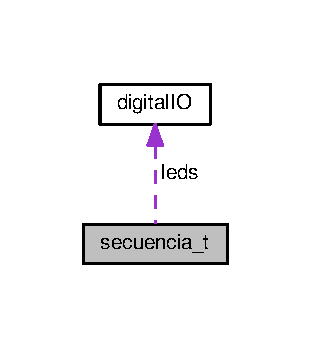
\includegraphics[width=149pt]{structsecuencia__t__coll__graph}
\end{center}
\end{figure}
\subsection*{Public Attributes}
\begin{DoxyCompactItemize}
\item 
\hyperlink{structdigital_i_o}{digital\+IO} {\bfseries leds} \mbox{[}max\+\_\+iter\mbox{]}
\item 
uint16\+\_\+t {\bfseries periodo}
\end{DoxyCompactItemize}


\subsection{Detailed Description}
Estructura que caracteriza una secuencia. 

The documentation for this struct was generated from the following file\+:\begin{DoxyCompactItemize}
\item 
inc/\hyperlink{operaciones_8h}{operaciones.\+h}\end{DoxyCompactItemize}

\chapter{File Documentation}
\hypertarget{hardware_8h}{}\section{inc/hardware.h File Reference}
\label{hardware_8h}\index{inc/hardware.\+h@{inc/hardware.\+h}}


Declaraciones de funciones y constantes simbólicas correspondientes con la E\+D\+U-\/\+C\+I\+AA N\+XP.  


{\ttfamily \#include \char`\"{}chip.\+h\char`\"{}}\\*
{\ttfamily \#include $<$stopwatch.\+h$>$}\\*
{\ttfamily \#include $<$stdint.\+h$>$}\\*
Include dependency graph for hardware.\+h\+:\nopagebreak
\begin{figure}[H]
\begin{center}
\leavevmode
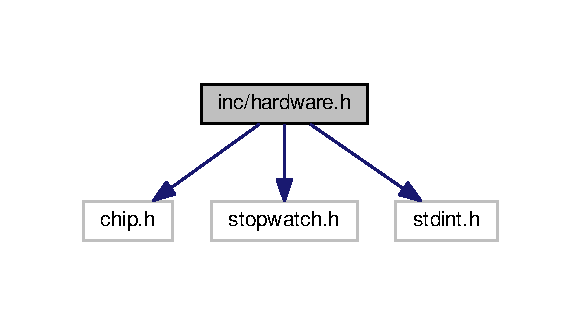
\includegraphics[width=279pt]{hardware_8h__incl}
\end{center}
\end{figure}
This graph shows which files directly or indirectly include this file\+:\nopagebreak
\begin{figure}[H]
\begin{center}
\leavevmode
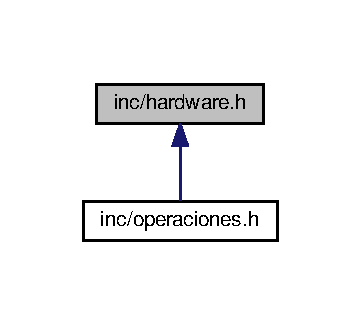
\includegraphics[width=173pt]{hardware_8h__dep__incl}
\end{center}
\end{figure}
\subsection*{Macros}
\begin{DoxyCompactItemize}
\item 
\#define \hyperlink{group__hardware_ga281151e2a661c8ad6893aee42b0024c4}{P\+O\+R\+T\+\_\+\+P\+I\+N\+\_\+\+L\+E\+D1}~0x02
\item 
\#define \hyperlink{group__hardware_ga1ee291f6ef730418abd5997176fe6b4c}{P\+I\+N\+\_\+\+L\+E\+D1}~0x0A
\item 
\#define \hyperlink{group__hardware_ga3039da47774de5edf9a11968103d87c5}{P\+O\+R\+T\+\_\+\+P\+I\+N\+\_\+\+L\+E\+D2}~0x02
\item 
\#define \hyperlink{group__hardware_gaa10e44027a1a9f0ac7cba19e815205a8}{P\+I\+N\+\_\+\+L\+E\+D2}~0x0B
\item 
\#define \hyperlink{group__hardware_ga097e347296860c96d104ef8ab90dac33}{P\+O\+R\+T\+\_\+\+P\+I\+N\+\_\+\+L\+E\+D3}~0x02
\item 
\#define \hyperlink{group__hardware_ga95a9a1b175a118c828537db81141eb3d}{P\+I\+N\+\_\+\+L\+E\+D3}~0x0C
\item 
\#define \hyperlink{group__hardware_ga372c868d523a46916b874b4e3c5722f5}{P\+O\+R\+T\+\_\+\+P\+I\+N\+\_\+\+R\+GB}~0x02
\item 
\#define \hyperlink{group__hardware_gaf3069b94e5b50d3558f6c36dd2e7ab15}{P\+I\+N\+\_\+\+R\+G\+B\+\_\+\+R\+ED}~0x00
\item 
\#define \hyperlink{group__hardware_ga298bb5d50ab2ba7b00df1c59087de286}{P\+I\+N\+\_\+\+R\+G\+B\+\_\+\+G\+RN}~0x01
\item 
\#define \hyperlink{group__hardware_gadf8d2d730566aede36c12ccfbc03b1b7}{P\+I\+N\+\_\+\+R\+G\+B\+\_\+\+B\+LU}~0x02
\item 
\#define \hyperlink{group__hardware_ga04c3e41fb79d2904c2358a42414bbf7f}{G\+P\+I\+O\+\_\+\+P\+O\+R\+T\+\_\+\+L\+E\+D1}~0x00
\item 
\#define \hyperlink{group__hardware_gaa4637d2cb87305ea71351291117a95f6}{G\+P\+I\+O\+\_\+\+P\+I\+N\+\_\+\+L\+E\+D1}~0x0E
\item 
\#define \hyperlink{group__hardware_gab971c6f67d136a9b870fac0f500685d4}{G\+P\+I\+O\+\_\+\+P\+O\+R\+T\+\_\+\+L\+E\+D2}~0x01
\item 
\#define \hyperlink{group__hardware_ga5ada73f73636a4fbf726468eb63eb945}{G\+P\+I\+O\+\_\+\+P\+I\+N\+\_\+\+L\+E\+D2}~0x0B
\item 
\#define \hyperlink{group__hardware_ga8b63f7f606f2b1ec7d88205ee6c514ea}{G\+P\+I\+O\+\_\+\+P\+O\+R\+T\+\_\+\+L\+E\+D3}~0x01
\item 
\#define \hyperlink{group__hardware_ga9e7e83187eae26d02136f609392fabd0}{G\+P\+I\+O\+\_\+\+P\+I\+N\+\_\+\+L\+E\+D3}~0x0C
\item 
\#define \hyperlink{group__hardware_ga9e2ed2756af597d0ec2ee618ef235c7e}{G\+P\+I\+O\+\_\+\+P\+O\+R\+T\+\_\+\+R\+GB}~0x05
\item 
\#define \hyperlink{group__hardware_gaa4aae4b49bb53e52b78b530637dcd2d7}{G\+P\+I\+O\+\_\+\+P\+I\+N\+\_\+\+R\+ED}~0x00
\item 
\#define \hyperlink{group__hardware_ga8ce252c71154210c65808a2170d74223}{G\+P\+I\+O\+\_\+\+P\+I\+N\+\_\+\+G\+RN}~0x01
\item 
\#define \hyperlink{group__hardware_ga2aa9b3c113e9f52a2e04ff811b8ec518}{G\+P\+I\+O\+\_\+\+P\+I\+N\+\_\+\+B\+LU}~0x02
\item 
\#define \hyperlink{group__hardware_gafe1bf3da61040955deda9703ee539687}{P\+O\+R\+T\+\_\+\+P\+I\+N\+\_\+\+K\+E\+Y1}~0x01
\item 
\#define \hyperlink{group__hardware_ga332cf72d49bf86b7b20274f3dec99d7b}{P\+I\+N\+\_\+\+K\+E\+Y1}~0x00
\item 
\#define \hyperlink{group__hardware_ga2cc4114181749a25732e31ed271a1f6b}{P\+O\+R\+T\+\_\+\+P\+I\+N\+\_\+\+K\+E\+Y2}~0x01
\item 
\#define \hyperlink{group__hardware_gae87128e49906c97fa9d6b438a08c1221}{P\+I\+N\+\_\+\+K\+E\+Y2}~0x01
\item 
\#define \hyperlink{group__hardware_ga5f697895be4580f403de4a9f75ab8a3b}{P\+O\+R\+T\+\_\+\+P\+I\+N\+\_\+\+K\+E\+Y3}~0x01
\item 
\#define \hyperlink{group__hardware_gaec621d9712815696a7bd342db8b2ff06}{P\+I\+N\+\_\+\+K\+E\+Y3}~0x02
\item 
\#define \hyperlink{group__hardware_gac86eb82e082d51cc0d4b0a87680cd7da}{P\+O\+R\+T\+\_\+\+P\+I\+N\+\_\+\+K\+E\+Y4}~0x01
\item 
\#define \hyperlink{group__hardware_gaf59a027359301b6e2229f7068c36efe6}{P\+I\+N\+\_\+\+K\+E\+Y4}~0x06
\item 
\#define \hyperlink{group__hardware_gabce59bc33538c850842e408765ae4981}{G\+P\+I\+O\+\_\+\+P\+O\+R\+T\+\_\+\+K\+E\+Y1}~0x00
\item 
\#define \hyperlink{group__hardware_ga26fa1a6916e027dcfa2d5a76c18dccb4}{G\+P\+I\+O\+\_\+\+P\+I\+N\+\_\+\+K\+E\+Y1}~0x04
\item 
\#define \hyperlink{group__hardware_gaeaf62bdfcf5fc1fe75d98d961286be78}{G\+P\+I\+O\+\_\+\+P\+O\+R\+T\+\_\+\+K\+E\+Y2}~0x00
\item 
\#define \hyperlink{group__hardware_ga6fe528c749e6e3df18c66c78841fd2ae}{G\+P\+I\+O\+\_\+\+P\+I\+N\+\_\+\+K\+E\+Y2}~0x08
\item 
\#define \hyperlink{group__hardware_ga6e75308c8b20c3236d0449a07bb052f7}{G\+P\+I\+O\+\_\+\+P\+O\+R\+T\+\_\+\+K\+E\+Y3}~0x00
\item 
\#define \hyperlink{group__hardware_ga6058161cd4273d1df2af95589e043055}{G\+P\+I\+O\+\_\+\+P\+I\+N\+\_\+\+K\+E\+Y3}~0x09
\item 
\#define \hyperlink{group__hardware_ga6d16f3a208324c46c462f92ad249d199}{G\+P\+I\+O\+\_\+\+P\+O\+R\+T\+\_\+\+K\+E\+Y4}~0x01
\item 
\#define \hyperlink{group__hardware_gabeaec154a7007cd91de9a8c775f4242f}{G\+P\+I\+O\+\_\+\+P\+I\+N\+\_\+\+K\+E\+Y4}~0x09
\item 
\#define \hyperlink{group__hardware_ga8dec203447e10cef9a4a1013f7c4cdd4}{next\+\_\+led}(x)~((x) = (x) $<$$<$ 1)
\begin{DoxyCompactList}\small\item\em Establece el siguiente valor en la enumeración \hyperlink{group__hardware_ga2a000bf02da2abba53355f3fcfdb2d0b}{board\+Leds}. \end{DoxyCompactList}\item 
\#define \hyperlink{group__hardware_ga6cc9878768b184e23371bbeb95360713}{prev\+\_\+led}(x)~((x) = (x) $>$$>$ 1)
\begin{DoxyCompactList}\small\item\em Establece el valor previo en la enumeración \hyperlink{group__hardware_ga2a000bf02da2abba53355f3fcfdb2d0b}{board\+Leds}. \end{DoxyCompactList}\item 
\#define \hyperlink{group__hardware_ga43a19ad1766c3719e591430d601496f7}{first\+\_\+led}~\hyperlink{group__hardware_gga84e58e8cc8e3fe349be97bcd3221c360a5662baf6795c7030ea75e47a0019a61d}{Led\+\_\+\+Rojo}
\begin{DoxyCompactList}\small\item\em Las definiciones fist\+Led, middle\+Led y last\+Led permiten encender los leds en secuencia desde el rgb Azul al led 3 (de middle\+Led a last\+Led) o la secuencia rojo, verde, azul al led 3 (utilizando de first\+Led a last\+Led). Estas definiciones permiten realizar operaciones como\+: \end{DoxyCompactList}\item 
\#define \hyperlink{group__hardware_gacbd2343998132167826e577781d85bbd}{middle\+\_\+led}~\hyperlink{group__hardware_gga84e58e8cc8e3fe349be97bcd3221c360a90357fded550cd38cda43991725234cb}{Led\+\_\+\+Azul}
\item 
\#define \hyperlink{group__hardware_ga6d4d3ee57587d8e08816b804150c29f8}{last\+\_\+led}~\hyperlink{group__hardware_gga2a000bf02da2abba53355f3fcfdb2d0ba16d63d90ec9dc8c27019e7c28ff1cfc0}{led3}
\item 
\#define \hyperlink{group__hardware_ga00c30099ff3ceab3e94a516833c11c98}{led\+On}(gpio\+Port,  gpio\+Pin)~Chip\+\_\+\+G\+P\+I\+O\+\_\+\+Set\+Pin\+State(L\+P\+C\+\_\+\+G\+P\+I\+O\+\_\+\+P\+O\+RT, gpio\+Port, gpio\+Pin, T\+R\+UE)
\begin{DoxyCompactList}\small\item\em Enciende un led. \end{DoxyCompactList}\item 
\#define \hyperlink{group__hardware_gac51bfbb3d5136e9e0479f3d8e6bb14de}{led\+Off}(gpio\+Port,  gpio\+Pin)~Chip\+\_\+\+G\+P\+I\+O\+\_\+\+Set\+Pin\+State(L\+P\+C\+\_\+\+G\+P\+I\+O\+\_\+\+P\+O\+RT, gpio\+Port, gpio\+Pin, F\+A\+L\+SE)
\begin{DoxyCompactList}\small\item\em Apaga un led. \end{DoxyCompactList}\item 
\#define \hyperlink{group__hardware_gaafb30c58d318e90ed902cb1aef013286}{led\+Toggle}(gpio\+Port,  gpio\+Pin)~Chip\+\_\+\+G\+P\+I\+O\+\_\+\+Set\+Pin\+Toggle(L\+P\+C\+\_\+\+G\+P\+I\+O\+\_\+\+P\+O\+RT, gpio\+Port, gpio\+Pin)
\begin{DoxyCompactList}\small\item\em Modifica el estado de un led particular (lo apaga si está encendido o lo enciende si está apagado). \end{DoxyCompactList}\item 
\#define \hyperlink{group__hardware_gafdd074f68e5ae5b133575140014f918d}{delay\+Ms}(x)~Stop\+Watch\+\_\+\+Delay\+Ms(x)
\begin{DoxyCompactList}\small\item\em Genera un delay de x milisegundos utilizando las primitivas del módulo \char`\"{}stopwatch\char`\"{} de lpc\+Open. \end{DoxyCompactList}\item 
\#define \hyperlink{group__hardware_ga1d13abaa815195d73e9dc2676e6fba5b}{delay\+Us}(x)~Stop\+Watch\+\_\+\+Delay\+Us(x)
\begin{DoxyCompactList}\small\item\em Genera un delay de x microsegundos utilizando las primitivas del módulo \char`\"{}stopwatch\char`\"{} de lpc\+Open. \end{DoxyCompactList}\end{DoxyCompactItemize}
\subsection*{Enumerations}
\begin{DoxyCompactItemize}
\item 
enum \hyperlink{group__hardware_ga8d70125ca4047f0f7ea513cd8568953d}{board\+Keys} \{ \hyperlink{group__hardware_gga8d70125ca4047f0f7ea513cd8568953da483a28cafb544915d9cd44f2c69fc706}{key1} =1, 
\hyperlink{group__hardware_gga8d70125ca4047f0f7ea513cd8568953dab8d9f65fc5604a8b8a0cdcbaf03bbbe0}{key2} =2, 
\hyperlink{group__hardware_gga8d70125ca4047f0f7ea513cd8568953da376c29473ae1a854ff46b2b171985093}{key3} =4, 
\hyperlink{group__hardware_gga8d70125ca4047f0f7ea513cd8568953da84011848209e666e74469d6dfba542eb}{key4} =8
 \}\begin{DoxyCompactList}\small\item\em Enumeración utilizada para identificar los pulsadores presentes en la E\+D\+U-\/\+C\+I\+AA N\+XP. \end{DoxyCompactList}
\item 
enum \hyperlink{group__hardware_ga84e58e8cc8e3fe349be97bcd3221c360}{rgb\+Leds} \{ \hyperlink{group__hardware_gga84e58e8cc8e3fe349be97bcd3221c360a5662baf6795c7030ea75e47a0019a61d}{Led\+\_\+\+Rojo} = 1, 
\hyperlink{group__hardware_gga84e58e8cc8e3fe349be97bcd3221c360aa5ad7834a37faf1e2620fa3db1838a21}{Led\+\_\+\+Verde} = 2, 
\hyperlink{group__hardware_gga84e58e8cc8e3fe349be97bcd3221c360a90357fded550cd38cda43991725234cb}{Led\+\_\+\+Azul} = 4
 \}\begin{DoxyCompactList}\small\item\em Enumeración asociada a los terminales de los leds R\+GB. \end{DoxyCompactList}
\item 
enum \hyperlink{group__hardware_ga2a000bf02da2abba53355f3fcfdb2d0b}{board\+Leds} \{ \\*
\hyperlink{group__hardware_gga2a000bf02da2abba53355f3fcfdb2d0ba76aaf0c615e41c008aa876ea4c183f4c}{led4} = Led\+\_\+\+Rojo, 
\hyperlink{group__hardware_gga2a000bf02da2abba53355f3fcfdb2d0ba66b97e4de94e08d049b57ac98e315cad}{led5} = Led\+\_\+\+Verde, 
\hyperlink{group__hardware_gga2a000bf02da2abba53355f3fcfdb2d0ba2c4a58277fd326a128900fe0904c2b1e}{led6} = Led\+\_\+\+Azul, 
\hyperlink{group__hardware_gga2a000bf02da2abba53355f3fcfdb2d0bacc803913e7d21f9a6900861008580c5f}{led1} = 8, 
\\*
\hyperlink{group__hardware_gga2a000bf02da2abba53355f3fcfdb2d0ba9c2c88fba1581ccd42348c9e3c47df92}{led2} = 16, 
\hyperlink{group__hardware_gga2a000bf02da2abba53355f3fcfdb2d0ba16d63d90ec9dc8c27019e7c28ff1cfc0}{led3} = 32
 \}\begin{DoxyCompactList}\small\item\em Enumeración utilizada para identificar los leds presentes en la E\+D\+U-\/\+C\+I\+AA N\+XP. \end{DoxyCompactList}
\end{DoxyCompactItemize}
\subsection*{Functions}
\begin{DoxyCompactItemize}
\item 
void \hyperlink{group__hardware_gab11a117f1e08391f23d1da05930e7acf}{system\+Init} (void)
\begin{DoxyCompactList}\small\item\em Inicializa los módulos básicos de la E\+D\+U-\/\+C\+I\+AA N\+XP. \end{DoxyCompactList}\item 
unsigned int \hyperlink{group__hardware_ga461352be081cdef66d03a73226849b41}{serial\+Write} (const uint8\+\_\+t $\ast$data, unsigned int data\+Len)
\begin{DoxyCompactList}\small\item\em Carga una cadena de caracteres para ser enviada a través de la U\+S\+A\+RT. Debe considerarse que la transmisión se realiza sin bloqueo y a través de interrupciones. Para eso, esta función invoca a Chip\+\_\+\+U\+A\+R\+T\+\_\+\+Send\+RB, la cuál copia la cadena en un buffer circular e inicia la transmición del primer caracter. Una vez disparada la interrupción que indica la finalización del envío, continúa con el siguiente caracter hasta que se completa la transmición de la cadena. \end{DoxyCompactList}\item 
void \hyperlink{group__hardware_gac20eca44aeea90e6f603831193cc9b28}{U\+A\+R\+T2\+\_\+\+I\+R\+Q\+Handler} (void)
\begin{DoxyCompactList}\small\item\em Obtiene los caracteres disponibles en el buffer circular asociado al flujo de entrada de caracteres (\char`\"{}lee el puerto\char`\"{}). \end{DoxyCompactList}\item 
void \hyperlink{group__hardware_ga4b6495dfec1dcc97e48043d7bca4da60}{set\+Led\+From\+Msk} (uint8\+\_\+t msk)
\begin{DoxyCompactList}\small\item\em Enciend o apaga un led según la máscara dada como argumento. \end{DoxyCompactList}\item 
void \hyperlink{group__hardware_ga3ac24a1bb2d63482077813f22c6930a1}{wait\+Key\+Press} (\hyperlink{group__hardware_ga8d70125ca4047f0f7ea513cd8568953d}{board\+Keys} \hyperlink{group__operaciones_ga3496dfc7a27df7eead65d48ed89e6867}{key})
\begin{DoxyCompactList}\small\item\em Espera a que se presione la tecla indicada a partir del argumento utilizado. \end{DoxyCompactList}\item 
uint8\+\_\+t \hyperlink{group__hardware_gabe9050eab201da85d14532c4d009603a}{get\+Key\+Pressed} (void)
\begin{DoxyCompactList}\small\item\em Retorna una máscara con el estado de las teclas. Si una tecla está presionada, retorna un bit en alto y si está suelta un bit en bajo. \end{DoxyCompactList}\end{DoxyCompactItemize}


\subsection{Detailed Description}
Declaraciones de funciones y constantes simbólicas correspondientes con la E\+D\+U-\/\+C\+I\+AA N\+XP. 

\begin{DoxyDate}{Date}
09/07/2018 
\end{DoxyDate}

\hypertarget{operaciones_8h}{}\section{inc/operaciones.h File Reference}
\label{operaciones_8h}\index{inc/operaciones.\+h@{inc/operaciones.\+h}}


Declaraciones de funciones y constantes simbólicas correspondientes con la E\+D\+U-\/\+C\+I\+AA N\+XP.  


{\ttfamily \#include \char`\"{}chip.\+h\char`\"{}}\\*
{\ttfamily \#include $<$stdio.\+h$>$}\\*
{\ttfamily \#include $<$stdlib.\+h$>$}\\*
{\ttfamily \#include $<$string.\+h$>$}\\*
{\ttfamily \#include $<$stopwatch.\+h$>$}\\*
{\ttfamily \#include \char`\"{}hardware.\+h\char`\"{}}\\*
Include dependency graph for operaciones.\+h\+:\nopagebreak
\begin{figure}[H]
\begin{center}
\leavevmode
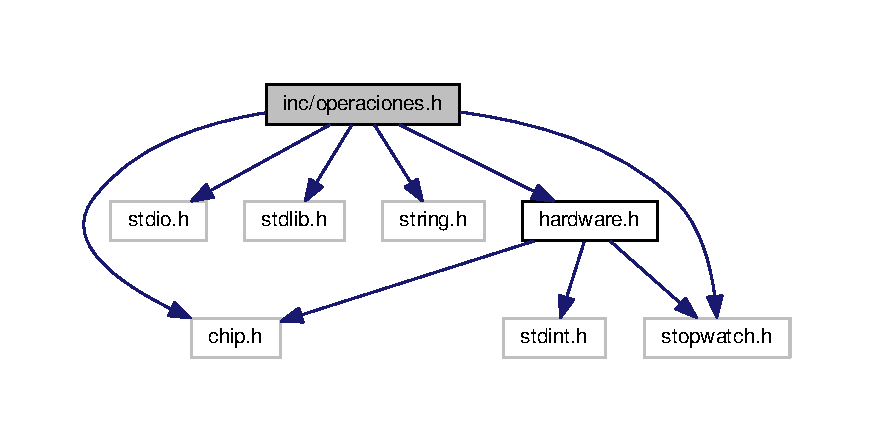
\includegraphics[width=350pt]{operaciones_8h__incl}
\end{center}
\end{figure}
\subsection*{Classes}
\begin{DoxyCompactItemize}
\item 
struct \hyperlink{structdigital_i_o}{digital\+IO}
\begin{DoxyCompactList}\small\item\em Estructuta utilizada para identificar los G\+P\+IO en la E\+D\+U-\/\+C\+I\+AA N\+XP, válido para los leds y los pulsadores Esta estructura permite definir un array de leds para simplificar la inicialización de los mismos, haciendo\+: \end{DoxyCompactList}\item 
struct \hyperlink{structsecuencia__t}{secuencia\+\_\+t}
\begin{DoxyCompactList}\small\item\em Estructura que caracteriza una secuencia. \end{DoxyCompactList}\end{DoxyCompactItemize}
\subsection*{Macros}
\begin{DoxyCompactItemize}
\item 
\#define {\bfseries T\+E\+C1\+\_\+\+I\+RQ}~1
\item 
\#define {\bfseries T\+E\+C2\+\_\+\+I\+RQ}~2
\item 
\#define {\bfseries T\+E\+C3\+\_\+\+I\+RQ}~3
\item 
\#define {\bfseries T\+E\+C4\+\_\+\+I\+RQ}~4
\item 
\#define \hyperlink{group__operaciones_ga571c3b0aaee2fe73b34cb9a7e26de731}{B\+U\+F\+F\+Size}~512
\item 
\#define {\bfseries primer\+\_\+led}~4
\item 
\#define {\bfseries segundo\+\_\+led}~8
\item 
\#define {\bfseries tercer\+\_\+led}~16
\item 
\#define {\bfseries ultimo\+\_\+led}~32
\item 
\#define {\bfseries max\+\_\+iter}~11
\end{DoxyCompactItemize}
\subsection*{Enumerations}
\begin{DoxyCompactItemize}
\item 
enum \hyperlink{group__operaciones_gac4035d04f315e3484218600aa1c52f44}{Board\+Keys} \{ \hyperlink{group__operaciones_ggac4035d04f315e3484218600aa1c52f44a5512d17c3218596367fffdc9bba5d772}{Key1} =4, 
\hyperlink{group__operaciones_ggac4035d04f315e3484218600aa1c52f44a4e2947c4588f93871e3321d6ed8b29ad}{Key2} =8, 
\hyperlink{group__operaciones_ggac4035d04f315e3484218600aa1c52f44ade464c5536012794d0bf75930adf611a}{Key3} =16, 
\hyperlink{group__operaciones_ggac4035d04f315e3484218600aa1c52f44aebb65f93ed25e808a5bfe10034f44e57}{Key4} =32
 \}\begin{DoxyCompactList}\small\item\em Enumeración utilizada para identificar los pulsadores presentes en la E\+D\+U-\/\+C\+I\+AA N\+XP. \end{DoxyCompactList}
\end{DoxyCompactItemize}
\subsection*{Functions}
\begin{DoxyCompactItemize}
\item 
void \hyperlink{group__operaciones_ga60b214b62e3bc463170aa71986a26a52}{inicializar\+\_\+sistema} (void)
\begin{DoxyCompactList}\small\item\em Inicializa los módulos básicos de la E\+D\+U-\/\+C\+I\+AA N\+XP. Los módulos configurados por esta función son\+: \end{DoxyCompactList}\item 
void \hyperlink{group__operaciones_gac2a7df7aa80e74c31cb5e7159ea3af26}{inicializar\+\_\+leds} (void)
\begin{DoxyCompactList}\small\item\em Inicializa los G\+P\+IO Leds Configura los pines asociados a los leds como salidas, estableciendo como valor inicial \char`\"{}apagado\char`\"{}. \end{DoxyCompactList}\item 
void \hyperlink{group__operaciones_ga03453754020d455c557635e866da3d4d}{inicializar\+\_\+teclado} (void)
\begin{DoxyCompactList}\small\item\em Inicializa los G\+P\+IO teclas Configura los pines asociadas a las teclas como entradas. \end{DoxyCompactList}\item 
void \hyperlink{group__operaciones_gaed73c66c75c4cfa90cb51636d371f6c1}{inicializar\+\_\+\+U\+S\+A\+RT} (void)
\begin{DoxyCompactList}\small\item\em configura la U\+S\+A\+R\+T2 U\+S\+A\+RT\+: configura la U\+S\+A\+R\+T2 utilizando interrupciones (115200/8/\+N/1). La configuración utilizada es transparente al usuario, la que el resultado del uso de interrupciones permite el envío y la recepción de caracteres sin bloqueo. \end{DoxyCompactList}\item 
void \hyperlink{group__operaciones_ga140cd744a440c2dc293252afbac6c2fc}{init\+\_\+interrupciones} (void)
\begin{DoxyCompactList}\small\item\em Función implementada para procesar las interrupciones del teclado. Esta función invoca a G\+P\+I\+O1\+\_\+\+I\+R\+Q\+Handler, G\+P\+I\+O2\+\_\+\+I\+R\+Q\+Handler, G\+P\+I\+O3\+\_\+\+I\+R\+Q\+Handler y G\+P\+I\+O4\+\_\+\+I\+R\+Q\+Handler correspondientes a cada una de las teclas de la E\+D\+U-\/\+C\+I\+AA N\+XP. \end{DoxyCompactList}\item 
void \hyperlink{group__operaciones_ga225d51b496ae1f1a31014cd1ff4de057}{display\+Counter} (uint8\+\_\+t v)
\begin{DoxyCompactList}\small\item\em Representa en los leds los 4 bits menos significativos del argumento v. Utiliza operadores a nivel de bit. \end{DoxyCompactList}\item 
void \hyperlink{group__operaciones_gaa9ec69e1f27876226ed140658228b324}{put\+Chr} (char $\ast$ch)
\begin{DoxyCompactList}\small\item\em Envia un carácter a través de la U\+S\+A\+R\+T2. \end{DoxyCompactList}\item 
void \hyperlink{group__operaciones_gaca6d6a4bbbd5abffc2dc954b9762672e}{print} (void $\ast$txt)
\begin{DoxyCompactList}\small\item\em Envia una cadena de caracteres a través de la U\+S\+A\+R\+T2. \end{DoxyCompactList}\item 
void \hyperlink{group__operaciones_gadc4ed2fec1b16a5a140e48f5fc4a35f0}{U\+S\+A\+R\+T\+Send\+Int} (uint8\+\_\+t integer)
\begin{DoxyCompactList}\small\item\em Envia enteros a traves de la U\+S\+A\+R\+T2. \end{DoxyCompactList}\item 
uint8\+\_\+t \hyperlink{group__operaciones_ga7f2a09c30550fe382fea806151b98a6e}{serial\+Read} (uint8\+\_\+t $\ast$data, uint8\+\_\+t max\+Data)
\begin{DoxyCompactList}\small\item\em Recibe datos a través de la U\+S\+A\+R\+T2 utilizando ringbuffers. \end{DoxyCompactList}\item 
void \hyperlink{group__operaciones_gaa0ad709d2e3ee927be33e7d380e70d02}{terminal\+\_\+eco} (void)
\begin{DoxyCompactList}\small\item\em Muestra por la terminal el valor que se ingresa. \end{DoxyCompactList}\item 
void \hyperlink{group__operaciones_ga06774e29c33f27100818e4d6729e53f5}{configurar\+\_\+\+Sys\+Tick} (void)
\begin{DoxyCompactList}\small\item\em Rutina para inicializar las interrupciones del System Tick Timer. \end{DoxyCompactList}\item 
void \hyperlink{group__operaciones_ga239ea5221c4ea3911f206a2fdb1e51f5}{disable\+\_\+\+Sys\+Tick} (void)
\begin{DoxyCompactList}\small\item\em Deshabilita el System Tick Timer. \end{DoxyCompactList}\item 
void \hyperlink{group__operaciones_gabc084d731c278381710d0f1b20064dd4}{escanear\+\_\+teclado} (void)
\begin{DoxyCompactList}\small\item\em Escanea el teclado y habilita los flags Pressed\+T\+E\+CX indicando la tecla que fue pulsada. \end{DoxyCompactList}\item 
void \hyperlink{group__operaciones_ga28acc17786e880e086680ffea93268e3}{generar\+\_\+secuencia} (void)
\begin{DoxyCompactList}\small\item\em Genera la secuencia de leds. \end{DoxyCompactList}\item 
uint32\+\_\+t \hyperlink{group__operaciones_ga58b590058ed8f7ffde70fcf916550750}{genera\+\_\+semilla} (void)
\begin{DoxyCompactList}\small\item\em Genera la semilla aleatoria para usar en la función srand La aletoriedad es implementada contando el número de ticks desde que se activa el Stop\+Watch hasta que se pulsa la tecla 1. \end{DoxyCompactList}\item 
void \hyperlink{group__operaciones_gad8987834f99880184b40422641c9c301}{evaluar\+\_\+secuencia} (void)
\begin{DoxyCompactList}\small\item\em Compara la secuencia ingresada con la generada Cuando se ingresa una secuencia de botones con igual número de elementos que la generada, evalua que haya sido la misma. \end{DoxyCompactList}\item 
void \hyperlink{group__operaciones_gac7e841cdb7e274872e259c1b28c738b6}{mostrar\+\_\+secuencia} (void)
\begin{DoxyCompactList}\small\item\em Muestra la secuencia del juego Recorre el vector de secuencias hasta la posicion (etapa) de juego y empieza cuenta regresiva para el ingreso de la secuencia. \end{DoxyCompactList}\item 
void \hyperlink{group__operaciones_ga4238c37f1c597d470eb9840113652cff}{titilar} (\hyperlink{structdigital_i_o}{digital\+IO} led, uint16\+\_\+t periodo, uint8\+\_\+t cant)
\begin{DoxyCompactList}\small\item\em Hace titilar un led en particular, una cierta cantidad de veces. \end{DoxyCompactList}\end{DoxyCompactItemize}
\subsection*{Variables}
\begin{DoxyCompactItemize}
\item 
unsigned char \hyperlink{group__operaciones_ga62ff739e128714bd8668fc1881669090}{rx\+Buff} \mbox{[}\hyperlink{group__operaciones_ga571c3b0aaee2fe73b34cb9a7e26de731}{B\+U\+F\+F\+Size}\mbox{]}
\item 
unsigned char \hyperlink{group__operaciones_gaecd7d757d466624f64f960512f1e46e7}{tx\+Buff} \mbox{[}\hyperlink{group__operaciones_ga571c3b0aaee2fe73b34cb9a7e26de731}{B\+U\+F\+F\+Size}\mbox{]}
\item 
R\+I\+N\+G\+B\+U\+F\+F\+\_\+T \hyperlink{group__operaciones_ga053907efdc46df32728b7a467638a604}{tx\+Ring}
\item 
R\+I\+N\+G\+B\+U\+F\+F\+\_\+T \hyperlink{group__operaciones_gab9788d6aaf5b45a37bf7384056801886}{rx\+Ring}
\item 
const \hyperlink{structdigital_i_o}{digital\+IO} \hyperlink{group__operaciones_ga9b625a8f4af05b1e2bdb0230a6440c77}{leds} \mbox{[}$\,$\mbox{]}
\begin{DoxyCompactList}\small\item\em Arreglo de leds. \end{DoxyCompactList}\item 
const \hyperlink{structdigital_i_o}{digital\+IO} \hyperlink{group__operaciones_ga827b5290b185d584f07107e0190dd6d2}{keys} \mbox{[}$\,$\mbox{]}
\begin{DoxyCompactList}\small\item\em Arreglo de pulsadores. \end{DoxyCompactList}\item 
\hyperlink{structsecuencia__t}{secuencia\+\_\+t} {\bfseries secuencia}
\item 
\hyperlink{structsecuencia__t}{secuencia\+\_\+t} {\bfseries secuencia\+\_\+ingresada}
\item 
uint8\+\_\+t {\bfseries pos\+\_\+secuencia}
\item 
uint8\+\_\+t {\bfseries pos\+\_\+ingreso}
\end{DoxyCompactItemize}


\subsection{Detailed Description}
Declaraciones de funciones y constantes simbólicas correspondientes con la E\+D\+U-\/\+C\+I\+AA N\+XP. 

\begin{DoxyDate}{Date}
15/09/2018 
\end{DoxyDate}

%--- End generated contents ---

% Index
\backmatter
\newpage
\phantomsection
\clearemptydoublepage
\addcontentsline{toc}{chapter}{Index}
\printindex

\end{document}
